
\documentclass[10pt]{article} % For LaTeX2e
\usepackage{tmlr}
%%\usepackage{showframe}
% If accepted, instead use the following line for the camera-ready submission:
% \usepackage[accepted]{tmlr}
% To de-anonymize and remove mentions to TMLR (for example for posting to preprint servers), instead use the following:
% \usepackage[preprint]{tmlr}

% Optional math commands from https://github.com/goodfeli/dlbook_notation.
%%%%% NEW MATH DEFINITIONS %%%%%

\usepackage{amsmath,amsfonts,bm}

% Mark sections of captions for referring to divisions of figures
\newcommand{\figleft}{{\em (Left)}}
\newcommand{\figcenter}{{\em (Center)}}
\newcommand{\figright}{{\em (Right)}}
\newcommand{\figtop}{{\em (Top)}}
\newcommand{\figbottom}{{\em (Bottom)}}
\newcommand{\captiona}{{\em (a)}}
\newcommand{\captionb}{{\em (b)}}
\newcommand{\captionc}{{\em (c)}}
\newcommand{\captiond}{{\em (d)}}

% Highlight a newly defined term
\newcommand{\newterm}[1]{{\bf #1}}


% Figure reference, lower-case.
\def\figref#1{figure~\ref{#1}}
% Figure reference, capital. For start of sentence
\def\Figref#1{Figure~\ref{#1}}
\def\twofigref#1#2{figures \ref{#1} and \ref{#2}}
\def\quadfigref#1#2#3#4{figures \ref{#1}, \ref{#2}, \ref{#3} and \ref{#4}}
% Section reference, lower-case.
\def\secref#1{section~\ref{#1}}
% Section reference, capital.
\def\Secref#1{Section~\ref{#1}}
% Reference to two sections.
\def\twosecrefs#1#2{sections \ref{#1} and \ref{#2}}
% Reference to three sections.
\def\secrefs#1#2#3{sections \ref{#1}, \ref{#2} and \ref{#3}}
% Reference to an equation, lower-case.
\def\eqref#1{equation~\ref{#1}}
% Reference to an equation, upper case
\def\Eqref#1{Equation~\ref{#1}}
% A raw reference to an equation---avoid using if possible
\def\plaineqref#1{\ref{#1}}
% Reference to a chapter, lower-case.
\def\chapref#1{chapter~\ref{#1}}
% Reference to an equation, upper case.
\def\Chapref#1{Chapter~\ref{#1}}
% Reference to a range of chapters
\def\rangechapref#1#2{chapters\ref{#1}--\ref{#2}}
% Reference to an algorithm, lower-case.
\def\algref#1{algorithm~\ref{#1}}
% Reference to an algorithm, upper case.
\def\Algref#1{Algorithm~\ref{#1}}
\def\twoalgref#1#2{algorithms \ref{#1} and \ref{#2}}
\def\Twoalgref#1#2{Algorithms \ref{#1} and \ref{#2}}
% Reference to a part, lower case
\def\partref#1{part~\ref{#1}}
% Reference to a part, upper case
\def\Partref#1{Part~\ref{#1}}
\def\twopartref#1#2{parts \ref{#1} and \ref{#2}}

\def\ceil#1{\lceil #1 \rceil}
\def\floor#1{\lfloor #1 \rfloor}
\def\1{\bm{1}}
\newcommand{\train}{\mathcal{D}}
\newcommand{\valid}{\mathcal{D_{\mathrm{valid}}}}
\newcommand{\test}{\mathcal{D_{\mathrm{test}}}}

\def\eps{{\epsilon}}


% Random variables
\def\reta{{\textnormal{$\eta$}}}
\def\ra{{\textnormal{a}}}
\def\rb{{\textnormal{b}}}
\def\rc{{\textnormal{c}}}
\def\rd{{\textnormal{d}}}
\def\re{{\textnormal{e}}}
\def\rf{{\textnormal{f}}}
\def\rg{{\textnormal{g}}}
\def\rh{{\textnormal{h}}}
\def\ri{{\textnormal{i}}}
\def\rj{{\textnormal{j}}}
\def\rk{{\textnormal{k}}}
\def\rl{{\textnormal{l}}}
% rm is already a command, just don't name any random variables m
\def\rn{{\textnormal{n}}}
\def\ro{{\textnormal{o}}}
\def\rp{{\textnormal{p}}}
\def\rq{{\textnormal{q}}}
\def\rr{{\textnormal{r}}}
\def\rs{{\textnormal{s}}}
\def\rt{{\textnormal{t}}}
\def\ru{{\textnormal{u}}}
\def\rv{{\textnormal{v}}}
\def\rw{{\textnormal{w}}}
\def\rx{{\textnormal{x}}}
\def\ry{{\textnormal{y}}}
\def\rz{{\textnormal{z}}}

% Random vectors
\def\rvepsilon{{\mathbf{\epsilon}}}
\def\rvtheta{{\mathbf{\theta}}}
\def\rva{{\mathbf{a}}}
\def\rvb{{\mathbf{b}}}
\def\rvc{{\mathbf{c}}}
\def\rvd{{\mathbf{d}}}
\def\rve{{\mathbf{e}}}
\def\rvf{{\mathbf{f}}}
\def\rvg{{\mathbf{g}}}
\def\rvh{{\mathbf{h}}}
\def\rvu{{\mathbf{i}}}
\def\rvj{{\mathbf{j}}}
\def\rvk{{\mathbf{k}}}
\def\rvl{{\mathbf{l}}}
\def\rvm{{\mathbf{m}}}
\def\rvn{{\mathbf{n}}}
\def\rvo{{\mathbf{o}}}
\def\rvp{{\mathbf{p}}}
\def\rvq{{\mathbf{q}}}
\def\rvr{{\mathbf{r}}}
\def\rvs{{\mathbf{s}}}
\def\rvt{{\mathbf{t}}}
\def\rvu{{\mathbf{u}}}
\def\rvv{{\mathbf{v}}}
\def\rvw{{\mathbf{w}}}
\def\rvx{{\mathbf{x}}}
\def\rvy{{\mathbf{y}}}
\def\rvz{{\mathbf{z}}}

% Elements of random vectors
\def\erva{{\textnormal{a}}}
\def\ervb{{\textnormal{b}}}
\def\ervc{{\textnormal{c}}}
\def\ervd{{\textnormal{d}}}
\def\erve{{\textnormal{e}}}
\def\ervf{{\textnormal{f}}}
\def\ervg{{\textnormal{g}}}
\def\ervh{{\textnormal{h}}}
\def\ervi{{\textnormal{i}}}
\def\ervj{{\textnormal{j}}}
\def\ervk{{\textnormal{k}}}
\def\ervl{{\textnormal{l}}}
\def\ervm{{\textnormal{m}}}
\def\ervn{{\textnormal{n}}}
\def\ervo{{\textnormal{o}}}
\def\ervp{{\textnormal{p}}}
\def\ervq{{\textnormal{q}}}
\def\ervr{{\textnormal{r}}}
\def\ervs{{\textnormal{s}}}
\def\ervt{{\textnormal{t}}}
\def\ervu{{\textnormal{u}}}
\def\ervv{{\textnormal{v}}}
\def\ervw{{\textnormal{w}}}
\def\ervx{{\textnormal{x}}}
\def\ervy{{\textnormal{y}}}
\def\ervz{{\textnormal{z}}}

% Random matrices
\def\rmA{{\mathbf{A}}}
\def\rmB{{\mathbf{B}}}
\def\rmC{{\mathbf{C}}}
\def\rmD{{\mathbf{D}}}
\def\rmE{{\mathbf{E}}}
\def\rmF{{\mathbf{F}}}
\def\rmG{{\mathbf{G}}}
\def\rmH{{\mathbf{H}}}
\def\rmI{{\mathbf{I}}}
\def\rmJ{{\mathbf{J}}}
\def\rmK{{\mathbf{K}}}
\def\rmL{{\mathbf{L}}}
\def\rmM{{\mathbf{M}}}
\def\rmN{{\mathbf{N}}}
\def\rmO{{\mathbf{O}}}
\def\rmP{{\mathbf{P}}}
\def\rmQ{{\mathbf{Q}}}
\def\rmR{{\mathbf{R}}}
\def\rmS{{\mathbf{S}}}
\def\rmT{{\mathbf{T}}}
\def\rmU{{\mathbf{U}}}
\def\rmV{{\mathbf{V}}}
\def\rmW{{\mathbf{W}}}
\def\rmX{{\mathbf{X}}}
\def\rmY{{\mathbf{Y}}}
\def\rmZ{{\mathbf{Z}}}

% Elements of random matrices
\def\ermA{{\textnormal{A}}}
\def\ermB{{\textnormal{B}}}
\def\ermC{{\textnormal{C}}}
\def\ermD{{\textnormal{D}}}
\def\ermE{{\textnormal{E}}}
\def\ermF{{\textnormal{F}}}
\def\ermG{{\textnormal{G}}}
\def\ermH{{\textnormal{H}}}
\def\ermI{{\textnormal{I}}}
\def\ermJ{{\textnormal{J}}}
\def\ermK{{\textnormal{K}}}
\def\ermL{{\textnormal{L}}}
\def\ermM{{\textnormal{M}}}
\def\ermN{{\textnormal{N}}}
\def\ermO{{\textnormal{O}}}
\def\ermP{{\textnormal{P}}}
\def\ermQ{{\textnormal{Q}}}
\def\ermR{{\textnormal{R}}}
\def\ermS{{\textnormal{S}}}
\def\ermT{{\textnormal{T}}}
\def\ermU{{\textnormal{U}}}
\def\ermV{{\textnormal{V}}}
\def\ermW{{\textnormal{W}}}
\def\ermX{{\textnormal{X}}}
\def\ermY{{\textnormal{Y}}}
\def\ermZ{{\textnormal{Z}}}

% Vectors
\def\vzero{{\bm{0}}}
\def\vone{{\bm{1}}}
\def\vmu{{\bm{\mu}}}
\def\vtheta{{\bm{\theta}}}
\def\va{{\bm{a}}}
\def\vb{{\bm{b}}}
\def\vc{{\bm{c}}}
\def\vd{{\bm{d}}}
\def\ve{{\bm{e}}}
\def\vf{{\bm{f}}}
\def\vg{{\bm{g}}}
\def\vh{{\bm{h}}}
\def\vi{{\bm{i}}}
\def\vj{{\bm{j}}}
\def\vk{{\bm{k}}}
\def\vl{{\bm{l}}}
\def\vm{{\bm{m}}}
\def\vn{{\bm{n}}}
\def\vo{{\bm{o}}}
\def\vp{{\bm{p}}}
\def\vq{{\bm{q}}}
\def\vr{{\bm{r}}}
\def\vs{{\bm{s}}}
\def\vt{{\bm{t}}}
\def\vu{{\bm{u}}}
\def\vv{{\bm{v}}}
\def\vw{{\bm{w}}}
\def\vx{{\bm{x}}}
\def\vy{{\bm{y}}}
\def\vz{{\bm{z}}}

% Elements of vectors
\def\evalpha{{\alpha}}
\def\evbeta{{\beta}}
\def\evepsilon{{\epsilon}}
\def\evlambda{{\lambda}}
\def\evomega{{\omega}}
\def\evmu{{\mu}}
\def\evpsi{{\psi}}
\def\evsigma{{\sigma}}
\def\evtheta{{\theta}}
\def\eva{{a}}
\def\evb{{b}}
\def\evc{{c}}
\def\evd{{d}}
\def\eve{{e}}
\def\evf{{f}}
\def\evg{{g}}
\def\evh{{h}}
\def\evi{{i}}
\def\evj{{j}}
\def\evk{{k}}
\def\evl{{l}}
\def\evm{{m}}
\def\evn{{n}}
\def\evo{{o}}
\def\evp{{p}}
\def\evq{{q}}
\def\evr{{r}}
\def\evs{{s}}
\def\evt{{t}}
\def\evu{{u}}
\def\evv{{v}}
\def\evw{{w}}
\def\evx{{x}}
\def\evy{{y}}
\def\evz{{z}}

% Matrix
\def\mA{{\bm{A}}}
\def\mB{{\bm{B}}}
\def\mC{{\bm{C}}}
\def\mD{{\bm{D}}}
\def\mE{{\bm{E}}}
\def\mF{{\bm{F}}}
\def\mG{{\bm{G}}}
\def\mH{{\bm{H}}}
\def\mI{{\bm{I}}}
\def\mJ{{\bm{J}}}
\def\mK{{\bm{K}}}
\def\mL{{\bm{L}}}
\def\mM{{\bm{M}}}
\def\mN{{\bm{N}}}
\def\mO{{\bm{O}}}
\def\mP{{\bm{P}}}
\def\mQ{{\bm{Q}}}
\def\mR{{\bm{R}}}
\def\mS{{\bm{S}}}
\def\mT{{\bm{T}}}
\def\mU{{\bm{U}}}
\def\mV{{\bm{V}}}
\def\mW{{\bm{W}}}
\def\mX{{\bm{X}}}
\def\mY{{\bm{Y}}}
\def\mZ{{\bm{Z}}}
\def\mBeta{{\bm{\beta}}}
\def\mPhi{{\bm{\Phi}}}
\def\mLambda{{\bm{\Lambda}}}
\def\mSigma{{\bm{\Sigma}}}

% Tensor
\DeclareMathAlphabet{\mathsfit}{\encodingdefault}{\sfdefault}{m}{sl}
\SetMathAlphabet{\mathsfit}{bold}{\encodingdefault}{\sfdefault}{bx}{n}
\newcommand{\tens}[1]{\bm{\mathsfit{#1}}}
\def\tA{{\tens{A}}}
\def\tB{{\tens{B}}}
\def\tC{{\tens{C}}}
\def\tD{{\tens{D}}}
\def\tE{{\tens{E}}}
\def\tF{{\tens{F}}}
\def\tG{{\tens{G}}}
\def\tH{{\tens{H}}}
\def\tI{{\tens{I}}}
\def\tJ{{\tens{J}}}
\def\tK{{\tens{K}}}
\def\tL{{\tens{L}}}
\def\tM{{\tens{M}}}
\def\tN{{\tens{N}}}
\def\tO{{\tens{O}}}
\def\tP{{\tens{P}}}
\def\tQ{{\tens{Q}}}
\def\tR{{\tens{R}}}
\def\tS{{\tens{S}}}
\def\tT{{\tens{T}}}
\def\tU{{\tens{U}}}
\def\tV{{\tens{V}}}
\def\tW{{\tens{W}}}
\def\tX{{\tens{X}}}
\def\tY{{\tens{Y}}}
\def\tZ{{\tens{Z}}}


% Graph
\def\gA{{\mathcal{A}}}
\def\gB{{\mathcal{B}}}
\def\gC{{\mathcal{C}}}
\def\gD{{\mathcal{D}}}
\def\gE{{\mathcal{E}}}
\def\gF{{\mathcal{F}}}
\def\gG{{\mathcal{G}}}
\def\gH{{\mathcal{H}}}
\def\gI{{\mathcal{I}}}
\def\gJ{{\mathcal{J}}}
\def\gK{{\mathcal{K}}}
\def\gL{{\mathcal{L}}}
\def\gM{{\mathcal{M}}}
\def\gN{{\mathcal{N}}}
\def\gO{{\mathcal{O}}}
\def\gP{{\mathcal{P}}}
\def\gQ{{\mathcal{Q}}}
\def\gR{{\mathcal{R}}}
\def\gS{{\mathcal{S}}}
\def\gT{{\mathcal{T}}}
\def\gU{{\mathcal{U}}}
\def\gV{{\mathcal{V}}}
\def\gW{{\mathcal{W}}}
\def\gX{{\mathcal{X}}}
\def\gY{{\mathcal{Y}}}
\def\gZ{{\mathcal{Z}}}

% Sets
\def\sA{{\mathbb{A}}}
\def\sB{{\mathbb{B}}}
\def\sC{{\mathbb{C}}}
\def\sD{{\mathbb{D}}}
% Don't use a set called E, because this would be the same as our symbol
% for expectation.
\def\sF{{\mathbb{F}}}
\def\sG{{\mathbb{G}}}
\def\sH{{\mathbb{H}}}
\def\sI{{\mathbb{I}}}
\def\sJ{{\mathbb{J}}}
\def\sK{{\mathbb{K}}}
\def\sL{{\mathbb{L}}}
\def\sM{{\mathbb{M}}}
\def\sN{{\mathbb{N}}}
\def\sO{{\mathbb{O}}}
\def\sP{{\mathbb{P}}}
\def\sQ{{\mathbb{Q}}}
\def\sR{{\mathbb{R}}}
\def\sS{{\mathbb{S}}}
\def\sT{{\mathbb{T}}}
\def\sU{{\mathbb{U}}}
\def\sV{{\mathbb{V}}}
\def\sW{{\mathbb{W}}}
\def\sX{{\mathbb{X}}}
\def\sY{{\mathbb{Y}}}
\def\sZ{{\mathbb{Z}}}

% Entries of a matrix
\def\emLambda{{\Lambda}}
\def\emA{{A}}
\def\emB{{B}}
\def\emC{{C}}
\def\emD{{D}}
\def\emE{{E}}
\def\emF{{F}}
\def\emG{{G}}
\def\emH{{H}}
\def\emI{{I}}
\def\emJ{{J}}
\def\emK{{K}}
\def\emL{{L}}
\def\emM{{M}}
\def\emN{{N}}
\def\emO{{O}}
\def\emP{{P}}
\def\emQ{{Q}}
\def\emR{{R}}
\def\emS{{S}}
\def\emT{{T}}
\def\emU{{U}}
\def\emV{{V}}
\def\emW{{W}}
\def\emX{{X}}
\def\emY{{Y}}
\def\emZ{{Z}}
\def\emSigma{{\Sigma}}

% entries of a tensor
% Same font as tensor, without \bm wrapper
\newcommand{\etens}[1]{\mathsfit{#1}}
\def\etLambda{{\etens{\Lambda}}}
\def\etA{{\etens{A}}}
\def\etB{{\etens{B}}}
\def\etC{{\etens{C}}}
\def\etD{{\etens{D}}}
\def\etE{{\etens{E}}}
\def\etF{{\etens{F}}}
\def\etG{{\etens{G}}}
\def\etH{{\etens{H}}}
\def\etI{{\etens{I}}}
\def\etJ{{\etens{J}}}
\def\etK{{\etens{K}}}
\def\etL{{\etens{L}}}
\def\etM{{\etens{M}}}
\def\etN{{\etens{N}}}
\def\etO{{\etens{O}}}
\def\etP{{\etens{P}}}
\def\etQ{{\etens{Q}}}
\def\etR{{\etens{R}}}
\def\etS{{\etens{S}}}
\def\etT{{\etens{T}}}
\def\etU{{\etens{U}}}
\def\etV{{\etens{V}}}
\def\etW{{\etens{W}}}
\def\etX{{\etens{X}}}
\def\etY{{\etens{Y}}}
\def\etZ{{\etens{Z}}}

% The true underlying data generating distribution
\newcommand{\pdata}{p_{\rm{data}}}
% The empirical distribution defined by the training set
\newcommand{\ptrain}{\hat{p}_{\rm{data}}}
\newcommand{\Ptrain}{\hat{P}_{\rm{data}}}
% The model distribution
\newcommand{\pmodel}{p_{\rm{model}}}
\newcommand{\Pmodel}{P_{\rm{model}}}
\newcommand{\ptildemodel}{\tilde{p}_{\rm{model}}}
% Stochastic autoencoder distributions
\newcommand{\pencode}{p_{\rm{encoder}}}
\newcommand{\pdecode}{p_{\rm{decoder}}}
\newcommand{\precons}{p_{\rm{reconstruct}}}

\newcommand{\laplace}{\mathrm{Laplace}} % Laplace distribution

\newcommand{\E}{\mathbb{E}}
\newcommand{\Ls}{\mathcal{L}}
\newcommand{\R}{\mathbb{R}}
\newcommand{\emp}{\tilde{p}}
\newcommand{\lr}{\alpha}
\newcommand{\reg}{\lambda}
\newcommand{\rect}{\mathrm{rectifier}}
\newcommand{\softmax}{\mathrm{softmax}}
\newcommand{\sigmoid}{\sigma}
\newcommand{\softplus}{\zeta}
\newcommand{\KL}{D_{\mathrm{KL}}}
\newcommand{\Var}{\mathrm{Var}}
\newcommand{\standarderror}{\mathrm{SE}}
\newcommand{\Cov}{\mathrm{Cov}}
% Wolfram Mathworld says $L^2$ is for function spaces and $\ell^2$ is for vectors
% But then they seem to use $L^2$ for vectors throughout the site, and so does
% wikipedia.
\newcommand{\normlzero}{L^0}
\newcommand{\normlone}{L^1}
\newcommand{\normltwo}{L^2}
\newcommand{\normlp}{L^p}
\newcommand{\normmax}{L^\infty}

\newcommand{\parents}{Pa} % See usage in notation.tex. Chosen to match Daphne's book.

\DeclareMathOperator*{\argmax}{arg\,max}
\DeclareMathOperator*{\argmin}{arg\,min}

\DeclareMathOperator{\sign}{sign}
\DeclareMathOperator{\Tr}{Tr}
\let\ab\allowbreak


\usepackage{hyperref}
\usepackage{url}

% My Packages
\usepackage{cleveref}
\usepackage{comment}
\usepackage{csvsimple}
\usepackage{datatool}
\usepackage{todonotes}[disable]
\usepackage{graphicx}
\usepackage{subcaption}
\newcommand{\todokdinline}[1]{\todo[color=red!20,inline]{{KD: \small #1}}}
\newcommand{\todokd}[1]{\todo[color=red!20]{{\small #1 -- Kasra}}}
% \newcommand{\todocainline}[1]{\todo[color=yellow!20,inline]{{CA: \small #1}}}
\newcommand{\todocm}[1]{\todo[color=green!40]{\small #1 -- Cynthia}}
\newcommand{\todocmi}[1]{\todo[inline,color=green!40]{\small #1 -- Cynthia}}
\newcommand{\todoff}[1]{\todo[color=blue!20]{\small #1 -- Frank}}
\newcommand{\todoffinline}[1]{\todo[inline,color=blue!20]{\small #1 -- Frank}}
\newcommand{\todoed}[1]{\todo[color=cyan!20]{\small #1 -- Ed}}

\newcommand{\CitationNeeded}[1]{{\textbf {\color{red}Cite #1}}}
\newcommand{\ProofRead}[1]{{\textbf {\color{red}Proofread please #1}}}
\newcommand{\Complete}[0]{{\textbf {\color{red}Complete it }}}
\newcommand{\Rephrase}[1]{{\textbf {\color{red}Rephrase please #1}}}
\newcommand{\TD}[1]{{\color{red}{\textbf{TODO}}} #1}
\newcommand{\OK}[1]{{\color{green}{\textbf{DONE}}} #1}
\newcommand{\ours}{\textsc{EMMA}}
% \newcommand{\ours}{\textsc{EMMA}}
\newcommand{\geom}{\textsc{Geometric Alignment}}
\newcommand{\supcon}{\textsc{SupCon}}

%%%%%%%%%%%%%%%%%%%%
% EDITING LINK: 
% https://www.overleaf.com/3575751412sjsdmszkxsyh
%%%%%%%%%%%%%%%%%%%%

\title{Multimodal Language Learning in the Face of Missing Modalities}
% \\ Extended Multimodal Alignment \\ Combining Geometric and classification ... }

% Authors must not appear in the submitted version. They should be hidden
% as long as the tmlr package is used without the [accepted] or [preprint] options.
% Non-anonymous submissions will be rejected without review.

\author{\name Kasra Darvish \email kasradarvish@umbc.edu \\
      \addr Department of Computer Science\\
      University of Maryland Baltimore County
      \AND
      \name Edward Raff \email Raff\_Edward@bah.com \\
      \addr University of Maryland Baltimore County \\
      Booz Allen Hamilton
      \AND
      \name Francis Ferraro \email ferraro@umbc.edu \\
      \addr University of Maryland Baltimore County
      \AND
      \name Cynthia Matuszek \email cmat@umbc.edu\\
      \addr University of Maryland Baltimore County \\
      CIFAR Fellow}

% The \author macro works with any number of authors. Use \AND 
% to separate the names and addresses of multiple authors.

\newcommand{\fix}{\marginpar{FIX}}
\newcommand{\new}{\marginpar{NEW}}

\def\month{MM}  % Insert correct month for camera-ready version
\def\year{YYYY} % Insert correct year for camera-ready version
\def\openreview{\url{https://openreview.net/forum?id=XXXX}} % Insert correct link to OpenReview for camera-ready version


\begin{document}


\maketitle



\begin{abstract}
    % Grounded language understanding, in which natural language is used as a query against objects in a physical environment, allows a real-world, intuitive mechanism by which users can instruct physical agents to engage in tasks such as object retrieval. Visuolinguistic approaches to such object inference tasks typically involve training on large pools of image/text pairs and then using language to subselect elements of the sensed environment. However, physical agents such as robots typically have access to sensory and interactive modalities beyond vision, and learning from multiple modalities can improve performance on downstream tasks. In order to fully leverage multimodal training data while being robust to missing information, we propose a generalized distance-based loss function that can be extended to learn retrieval models that incorporate an arbitrary number of modalities. We demonstrate the usability of our model on a grounded language object retrieval scenario, where an intelligent agent has to select an object given an unconstrained language command. We leverage four modalities including vision, depth sensing, text, and speech, and we show that our model can outperform state-of-the-art contrastive models when modalities are ablated.

    % shorter version
    
    We propose \textit{extended multimodal alignment (EMMA)}, a generalized geometric method combined with a cross-entropy loss function that can be used to learn retrieval models that incorporate an arbitrary number of views of a particular piece of data, compounded by the challenge of retrieval when a modality becomes unavailable. Our study is motivated by needs in robotics and computer-human interaction, where an agent has many sensors and thus modalities with which a human may interact, both to communicate a desired goal and for the agent to recognize a desired target object. For such problems, there has been little research on integrating more than two modalities. While there have been widely popular works on self-supervised contrastive learning based on cross-entropy, there is an entirely separate family of approaches based on explicit geometric alignment. However, to the best of our knowledge there has been no work on combining the two approaches for multimodal learning. We propose to combine both families of approaches and argue that the two are complementary. We demonstrate the usability of our model on a grounded language object retrieval scenario, where an intelligent agent has to select an object given an unconstrained language command. We leverage four modalities including vision, depth sensing, text, and speech, and we show that our model converges approximately 5 times faster than previous strong baselines, and out-performs or is strongly competitive with state-of-the-art contrastive learning. % (in 80\% less time).
    %when modalities are ablated. 
    The code is publicly available on GitHub and will be included for the camera-ready version (it is redacted for anonymity). 
\end{abstract}



\section{Introduction}
\label{intro}

Inspired by the multimodal nature of human interaction with the world, it is intuitive that agents learning about the world, upon encountering new concepts and new objects, should form a model that incorporates information from all available sensors and data sources. The benefits of integrating multiple modalities are twofold; first, complementary information can be extracted from different modalities that can help with understanding the world, and second, additional modalities can help in the cases when one or more sources of data about the world become unavailable.
% 
Grounded language understanding, in which natural language is used as a query against objects in a physical environment, allows a real-world, intuitive mechanism by which users can instruct physical agents to engage in tasks such as object retrieval. Visuolinguistic approaches to such object inference tasks typically involve training on large pools of image/text pairs and then using language to subselect elements of the sensed environment~\citep{hong2021gilbert,Zhuge_2021_CVPR_VLP}.

Although physical agents such as robots typically have access to sensory and interactive modalities beyond vision, and learning from multiple modalities can improve performance on downstream tasks, most approaches use at most two sensory inputs (e.g., visual data such as RGB plus depth images) with single labels, such as those provided by textual natural language. Simultaneously using additional inputs from different modalities is an underexplored area, in part due to the domain-specific nature of such \textit{n}-ary learning approaches. With the modern proliferation of audio and text based communication and home agents (e.g., Alexa/Google Home), there is a growing need to handle more modalities, and simultaneously their potential failures. 

One difficulty with working with complex multimodal data is the increased likelihood that one or more modalities may have missing information. Hardware can become damaged or defective, sensors can get blocked or obstructed, and various adverse but not uncommon conditions can remove a modality from use.
Current multimodal approaches are typically not robust to the loss of one or more modalities at test time, as may happen if, for example, a physical agent fails to retrieve data from a particular sensor. In order to fully leverage multimodal training data while being robust to missing information, we propose a generalized distance-based loss function that can be extended to learn retrieval models that incorporate an arbitrary number of modalities.

We consider the domain of grounded language-based object retrieval~\citep{hu2016natural, triplet_loss_2021_CVPR}, in which objects in an environment must be identified based on linguistic instructions. This can be considered a special case of image retrieval~\citep{huang2017deep, ma2020large, novak2015large, vo2019composing} in which objects are identified using visual inputs in combination with other sensor modalities. Approaches to acquiring grounded language have explored various combinations of sensor inputs such as depth and RGB with labels provided by textual language or  speech~\citep{RichardsDarvishMatuszekCategoryFree20}. 
However, despite the multisensory nature of object retrieval, much of the existing work has not previously been extended to include an arbitrary number of modalities. 

% \todo[inline]{Whats the name of our method? When I skim the paper its hard to tell what ``the new thing is'', and then I have to read. I think being explicit here, with something like ``\textit{we propose our new method BLA}'' will help -Ed}

The ultimate aim of this work is to take arbitrary input modalities about novel objects, including both spoken and written language, and build a model that allows a system to correctly retrieve that object given a subset of those input modalities. In this work, we propose our new method \ours{}, a generalized geometric method combined with a cross-entropy loss function that can be used to learn retrieval models that incorporate an arbitrary number of views of a particular piece of data. We demonstrate steps towards this ultimate goal with a mechanism that learns quickly from a variety of input signals and is robust to ablation of certain inputs. This is a generalization of approaches to grounded language learning in which specific input modalities are labeled with language to allow for future identification, but explicitly seeks to be agnostic about the nature of the individual sensory and linguistic inputs. 

Our contributions are as follows:
\begin{enumerate}
    \item Proposing a new approach to multimodal learning by combining geometric and cross-entropy methods and showing that it outperforms and converges faster compared to each method separately.
    % \item Outperforming state-of-the-art models for grounded language learning by differentiating visual input modalities such as RGB and depth, rather than combining them into a single modality.
    
    \item Our method is designed to be applicable to additional modalities as they become available.

    \item Our method converges approximately 5 times faster than previous strong baselines, and out-performs or is strongly competitive with state-of-the-art contrastive learning~\citep{chen2020simple} and supervised contrastive learning~\citep{NEURIPS2020_supervised_contrastive} models when all modalities are available.

    \item Demonstrating robustness in the face of missing input signals when one or more modalities are ablated at test time, and proposing a simple averaging method to quantify performance for multimodal object retrieval scenarios.
    
    \item Demonstrating the separate utility of speech and text as sources of label information by treating them as sensory input modalities, rather than explicitly as labels.
    
    % \item Stable model that outperforms state-of-the-art contrastive learning models when batch size decreases.\todoff{add motivation in the intro about why robustness to a smaller batch size is important}
    
\end{enumerate}

% \todoffinline{Super pet peeve of mine: except for books or theses, don't take up space with this roadmap. Instead, in the above contributions, add pointers to the sections (or even subsections) where we provide evidence for each contribution}
% \todokdinline{I think Cynthia added this part for the last submission since we were short a few sentences to reach the page limit. We can remove this.}
% The remainder of this paper is organized as follows. In \cref{sec:Related-Work}, we describe existing work on visuolinguistic retrieval, contrastive learning, and multimodal learning. In \cref{sec:Problem-Description}, we formalize the object retrieval problem and give examples of the data under consideration. In \cref{sec:Method}, we describe our novel approach to learning models of linguistically-driven queries against a multimodal set of objects. Finally, in \cref{sec:Experiments}, we demonstrate the effectiveness of our approach against traditional contrastive learning and supervised contrastive learning baselines, both for the general learning problem and in the case of missing information at test time.

% \todocmi{NOTES: Some things are probably less informative or more ambiguous (e.g., depth for differentiating round things). So instead of predicting a single vector output, predict a vector and a covariance that captures uncertainty; could potentially use that to do more accurate search, or to handle really uncertain modalities (e.g., just drop speech when it's uninformative).} 

%===================================================================

\section{Related Work}
\label{sec:Related-Work}

% \todoffinline{I'm not convinced this section shouldn't appear toward the end of the paper. Maybe adding that narrative structure will help?}

% \todocmi{I'm not sure what narrative structure is being referred to here. I have a preference for having related work sections towards the beginning.}

There is extensive work on the task of image retrieval, of which physical object retrieval can be considered a special case. In this task, language is used to formulate queries against datasets of images, for example in text-and-image matching tasks for fashion data~\citep{gao2020fashionbert, wen2021comprehensive}, sketch retrieval~\citep{huang2017deep}, and general photographs of objects~\citep{ma2020large, novak2015large, hong2021gilbert}. Prior work has focused solely on language and visual modalities, using text or a combination of language and vision to perform visual retrieval~\citep{vo2019composing}. While recent works have focused on grounding with respect to a knowledge set \citep{10.1145/3357384.3357889,10.1145/3397271.3401097}, our work focuses on robust multimodal learning to perform grounding over an arbitrary number of input modalities. 

The growing number of datasets that contain modalities beyond images and text demonstrates the importance and the challenge of this task. \citet{bagher-zadeh-etal-2018-multimodal} introduce a large dataset of multimodal opinion sentiment and emotion intensity (CMU-MOSEI) for sentiment analysis and emotion recognition. They also introduce a novel multimodal fusion technique called the Dynamic Fusion Graph (DFG).~\citet{GoLD_UMBC} present a multimodal dataset of household objects containing RGB images, depth images, written language, and spoken language, which has been used to support learning grounded language directly from speech given small datasets~\citep{KebeAAAI2022}. 
\citet{baltrusaitisMultimodalMachineLearning2019} propose a new taxonomy of multimodal machine learning by introducing five technical challenges in addition to typical early and late fusion categorization. They cover different approaches to multimodal machine learning such as \textit{representation}, \textit{translation}, \textit{alignment}, \textit{fusion}, and \textit{co-learning}. In this work, we focus on alignment, the process of identifying the direct relationship between elements across modalities.

We highlight a key difference with recent work like \citet{10.1145/3397271.3401232} and \citet{10.1145/3331184.3331213} who develop multi-modal retrieval models. These retrieval models are class based, where the model is trained to recognize any object of the same retrieval class as being the `same.' Our method and data is instance based, where different objects are not considered the same even if they have the same class, due to the grounding goals of our work (i.e., the agent should identify the specified object, not equivalent objects). These works also do not consider performance in the case of failure of an input modality. 

A number of different approaches have been proposed for linguistic-based alignment learning. \citet{alayrac2020self} use a self-supervised contrastive learning method to learn and combine representations from three modalities of visual, audio, and language. Audio and visual domains are mapped to the same space because they are fine-grained, containing dense information for each frame of video, and these embeddings are then mapped to a coarse space where text is also mapped. Their network respects specificity and comparability of different modalities. The loss function they define consists of two distance-based terms for the corresponding spaces, differing from ours in that they do not handle arbitrarily many modalities and do not focus on robustness in the face of modality drop-outs. \citet{Nguyen-RSS-20} take a similar approach and perform pairwise cosine similarity to align images and natural language text descriptions to perform object retrieval tasks. \citet{triplet_loss_2021_CVPR} take a cross-modal manifold alignment approach to grounded language learning using triplet loss \citep{Chechik:2010:LSO:1756006.1756042}, and perform object retrieval by connecting text descriptions of objects to their corresponding RGB-D images.

In general there are two different families of approaches to multimodal learning in the literature. One family is based on classification and cross-entropy losses such as~\citet{NEURIPS2020_supervised_contrastive, chen2020simple} and the other family is geometric based such as~\citet{ICML22GeometricMultimodal,Carvalho-cooking-triplet,salvador2017cooking,triplet_loss_2021_CVPR}.
In this paper we propose to marry the two families and show that combining geometric approach with cross-entropy method is superior.

% \todokdinline{Should we move the following two paragraphs to the Approach section?}
% \todocmi{Actually yes, although I think it's more like 3 paragraphs. Rewriting the subsequent paragraphs so they don't appear out of nowhere would help.}
% \todokdinline{After moving baselines to the approach section and rewriting it, I think it's better if we leave these here. Let me know if you think otherwise.}

% For the classification part of our loss function we employ the supervised contrastive loss proposed by~\citet{NEURIPS2020_supervised_contrastive}. 
The way we formulate our geometric loss function is similar to lifted structured loss~\citep{songCVPR16LiftedStructured}, where they take a geometric approach in a unimodal scenario and consider pairwise distances among all items in a batch, but in this paper we apply our idea to four modalities, and our formulation can be extended to any number of modalities.
This extended geometric formulation results in a loss function that is similar to \citet{ICML22GeometricMultimodal} where they propose a geometric contrastive learning approach in which they %use the same instance of an MLP network (same weights) after extracting embeddings from each modality, while we use different instances of the same MLP network (different weights). They also 
fuse all embeddings as a central embedding and then minimize the distance between each embedding and that central embedding. However, their method does not take into account any notion of classification.

The geometric approach is also known as contrastive learning~\citep{qin2021world}, which is based on the idea of similarity and distance of elements of training data~\citep{Carvalho-cooking-triplet,triplet_loss_2021_CVPR,salvador2017cooking}. Triplet loss is also a special case of contrastive loss~\citep{NEURIPS2020_supervised_contrastive}. Contrastive loss is mostly used in self-supervised learning~\citep{bui2021self, alayrac2020self,chen2020simple}, with some exceptions such as \citet{NEURIPS2020_supervised_contrastive}, who use contrastive loss for a supervised problem. Most of these methods are implemented for a non-multimodal dataset (e.g., RGB images only). Our work is a specialization of contrastive loss that is focused on the multimodal input and language problem.

We note in particular that standard triplet learning approaches often require an expensive \textit{mining} step to find harder negative samples to enable effective learning \citep{Hoffer2015,Schroff2015,DBLP:conf/eccv/2018-9,DBLP:conf/eccv/ZhaoJQLH18,Zhai2018}. This is problematic for throughput and scalability, as run time becomes quadratic in batch size. Our approach does not require mining to obtain good performance, alleviating these issues along with their complicated history in reproducibility and parameter tuning \citep{Musgrave2020,Raff2020c,Raff2019_quantify_repro}. 

Some of the most closely related work focuses on learning based on more than two input modalities. \citet{Veit_2018_CVPR} train a joint model of images, hashtags, and users to perform image retrieval. Their task is similar to ours---given a description, we want to find the image/object in the scene that best matches the description. They tackle this problem by forming a three-way tensor product model. They use a ranking loss to train the model where the score of an observed triplet is higher than an unobserved triplet. They sample six negative triplets per positive sample triplet, and use each of them as a negative in the loss. The downstream retrieval task is then simply done by taking the argmax of the tensor product for a given user. This work differs from ours in that it becomes computationally complex as more and higher-dimensional modalities are added.
Our proposed geometric loss function resembles work on quadruplet loss~\citep{chen2017beyond,tursun2021efficient} but is intended to scale to an arbitrary number of modalities.

To the best of our knowledge, there has been limited work on incorporating more than three modalities into a general learning approach. \citet{semihet_three_way_Lei_2020} use inputs from three modalities of image, sketch, and edgemap to perform image retrieval given the sketch. They use a co-attention mechanism, and their loss function contains alignment loss, cross-entropy loss, and sketch-edgemap contrastive loss. \citet{Mittal2020M3ER} use Canonical Correlational Analysis (CCA) to differentiate between ineffective and effective modalities for the emotion recognition task from multiple input modalities including face, speech, and text. Multimodal learning has been used for different applications including but not limited to object retrieval. \citet{Deception_ICMI_2014} use language, physiological response, and thermal sensing to detect deceit. \citet{het_data_fusion_liu_IEEE_2017} take two modalities as input and output predictions in a third modality. \citet{tursun2021efficient} uses quadruplet loss for two modalities only; image and sketch. A quadruplet is composed of a sketch picture as an anchor, a negative example from sketch domain, a negative example from picture domain, and a positive example from picture domain. \citet{chen2017beyond} also uses quadruplet loss, but does not support multiple domains. In contrast, our method is not restricted to two modalities.
% \todo[inline]{talk about CLIP and DALL-E here}
 


%===================================================================

\section{Problem Description}
\label{sec:Problem-Description}

Given a language command (either text or speech) that describes an object, we want our model to retrieve the correct object from a set of objects. This problem is an exemplar of tasks found in the area of grounded language learning in the fields of robotics and natural  language processing. Intuitively, the goal is to take unconstrained natural language queries and select the appropriate object based on the complete set of sensor inputs available to the agent. We demonstrate on a domain containing four modalities, all of which refer to objects in the environment: spoken language, written text, RGB (image) inputs, and depth camera inputs. \Cref{fig:experimental-setup} illustrates a small visualization of our object retrieval task: the spoken query ``A white textbook titled algorithms'' is provided to our contrastive model, which identifies the item 
(outlined in red in \cref{fig:experimental-setup}) 
as the most likely item the query is referring to.

\begin{figure}[tb]
\centering
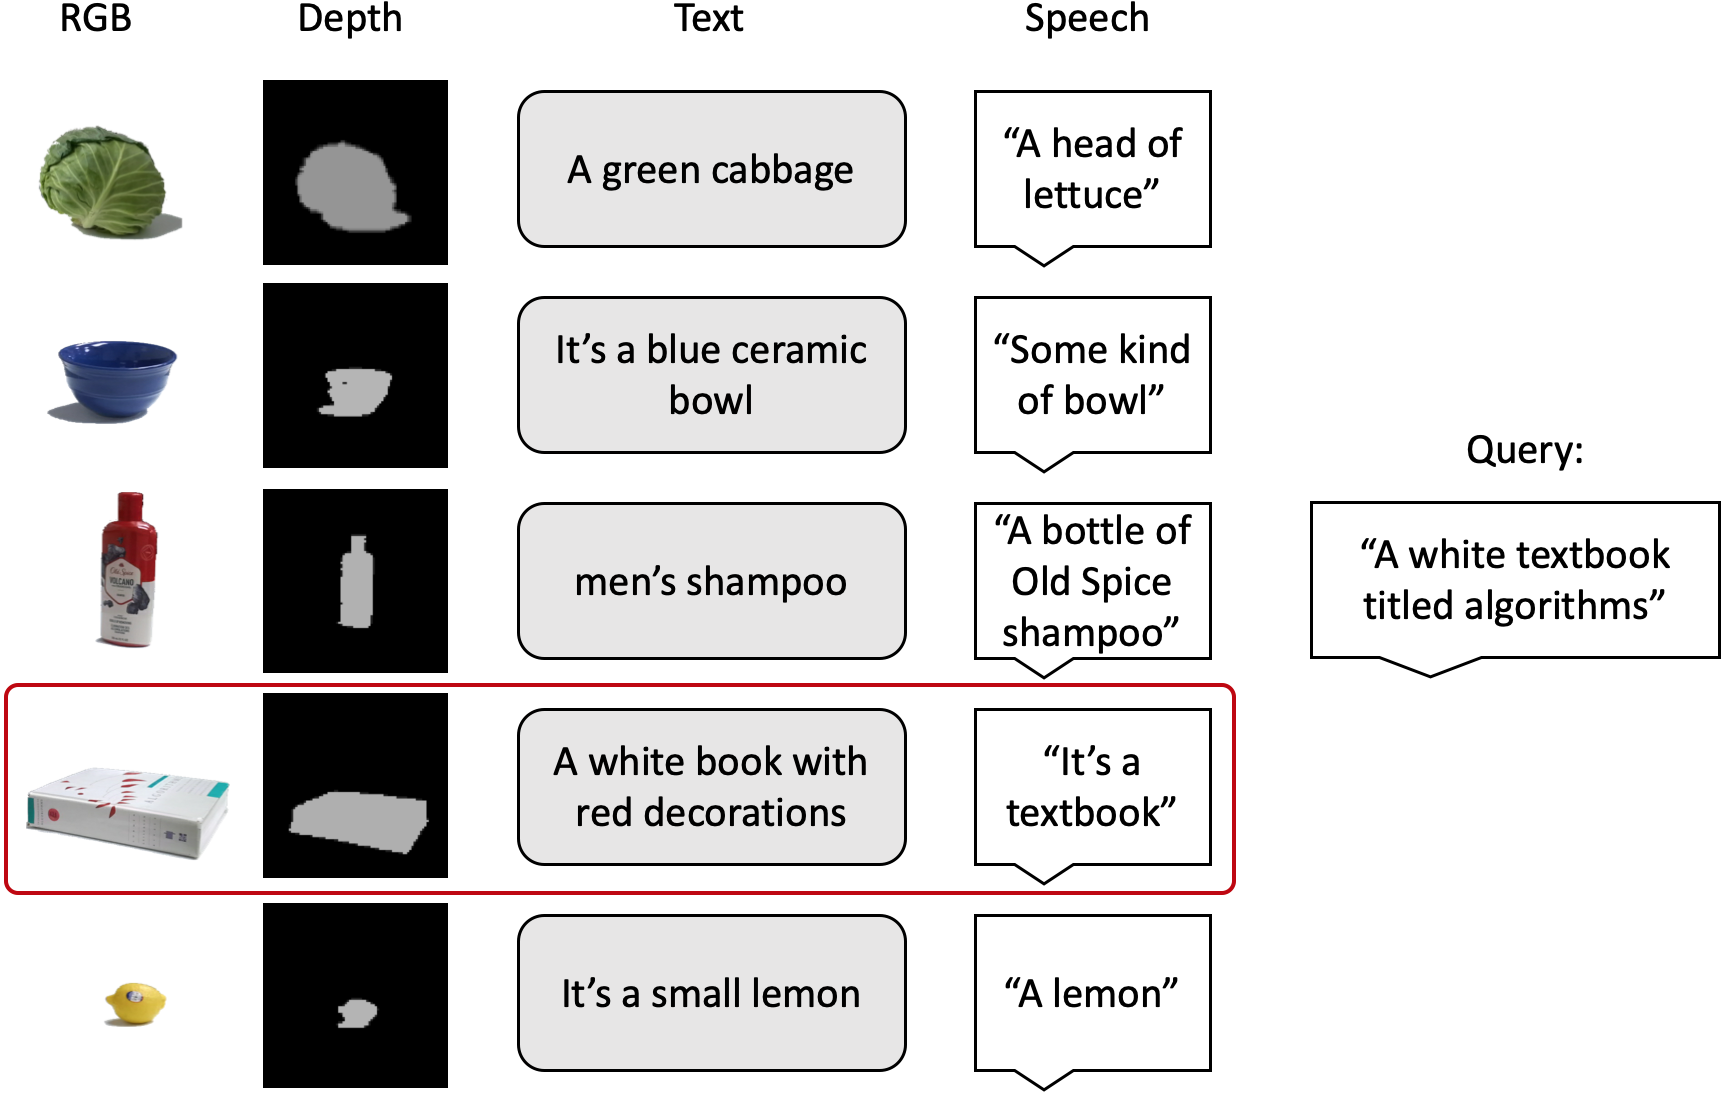
\includegraphics[width=.75\columnwidth]{Figures/experiment-setup-rearranged.png}
\caption{
The experimental object retrieval setup, in which objects are represented by four modalities: an RGB image, a depth image, spoken descriptions, and textual descriptions. Given a query in some modality, our approach seeks to select the object that is the best fit, per a trained model. This approach, detailed in \cref{sec:Method}, is able to rank objects as to appropriateness even when one or more modalities is ablated at test time (e.g., depth inputs are missing), and outperforms state-of-the-art contrastive learning approaches.
}
\label{fig:experimental-setup}
\end{figure}

More formally, given a spoken language command $x_s$, a textual language command $x_t$, a set of RGB images $X_r = \{x_r^{(1..n)}\}$, and a set of depth images $X_d = \{x_d^{(1..n)}\}$, the task is to retrieve the correct object by choosing the index that has the minimum distance from either of the language commands across all modalities.
Depending on which modalities are or are not ablated, we consider up to four distances: \textit{sr}, a vector of distances between $x_s$ and all RGB images in $X_r$; \textit{sd}, a vector of distances between $x_s$ and all depth images in $X_d$; \textit{tr}, a vector of distances between $x_t$ and all RGB images in $X_r$; and \textit{td}, a vector of distances between $x_t$ and all depth images in $X_d$. In order to select the correct object, we first perform a component-wise average of the relevant modality pair distances for the available modalities. Then, we select the object which had the minimum distance, i.e., we perform an argmin on this average vector of multiple-modality distances. Depending on the missing/available sensors during test time, we might have any combination of these four distances. For example, if no written instructions are available at test time,\footnote{This setting is particularly salient. While large bodies of text are frequently available at training time, a person interacting directly with a physical agent may well prefer to use only spoken instructions.} we compute the component-wise average of $sr$ and $sd$, and then select the object whose coordinate resulted in the lowest average distance. This method allows us to extend our model to support arbitrary modalities while remaining robust to test cases in which some modalities are missing or incomplete. 


%===================================================================

\section{Approach}
\label{sec:Method}

In keeping with previous work on the closely related problem of image retrieval, we focus on contrastive loss approaches, in which the goal is to learn an embedding of data where similar samples---in our case, samples belonging to the same class of object---are embedded `close' to one another, while dissimilar samples are farther apart. We develop a novel geometric loss function, \geom{}, that simultaneously minimizes intra-class distances and maximizes inter-class distances across each pair of modalities, yielding a model that is both effective at the retrieval task defined above and robust to modality dropouts at test time. We take an additional step and combine this \geom{} loss with a classification-based (cross-entropy) loss function which results in a superior model compared to either of geometric or cross-entropy losses alone; we refer to this combination as Extended Multi-Modal Alignment, or \ours{}.


\subsection{Baselines}
We compare both \ours{} and \geom{} against contrastive learning~\citep{chen2020simple} and supervised contrastive learning~\citep{NEURIPS2020_supervised_contrastive}, which for conciseness we refer to as \supcon{}.
We consider \supcon{} as the main baseline since it is a general version of multiple contrastive loss functions including triplet loss, the traditional version of contrastive loss usually used in self-supervised settings~\citep{chen2020simple}, and N-pair loss~\citep{NIPS2016N-PairLoss}.
% and do not include N-pair and triplet loss in our comparisons.
%contrastive learning methods including triplet loss, the traditional version of contrastive loss usually used in self-supervised settings~\citep{chen2020simple}, and supervised contrastive learning~\citep{NEURIPS2020_supervised_contrastive}. 




\begin{comment}
\subsubsection{Triplet Loss}
\label{sub:baseline-triplet}
Triplet loss has two major disadvantages. First, it cannot be used for more than two modalities.
Second, a batch size of greater than 1 is hard to implement if the anchor, positive, and negative come from different modalities for each batch.
% To address these issues in EMMA, we sample more than one positive and negative data points.
%Intuitively, we sample one positive data point and one negative data point, each of which includes $M$ modalities, resulting in 2M data points. Each of the $M$ positives modalities become an anchor once. 
% \Cref{table:quantitative} shows that our MMA method perform as good as this baseline while our model can be trained 10x faster since we can use batch sizes larger than 1. Also, 

% When we used a fixed anchor modality, a batch size of 64, and applied semantic negative sampling~\citep{Pillai_Matuszek_2018}, our method outperformed this baseline. However, 
% Since this method cannot be applied to four modalities, we do not include it in the main analysis. 
\end{comment}

\subsubsection{Contrastive Loss}
\label{sub:baseline-contrastive}


We compare our model against the contrastive learning method presented by~\citet{chen2020simple} where they use the normalized
temperature-scaled cross entropy loss (NT-Xent). In order to implement this loss function, we use cosine similarity as suggested in the SimCLR paper~\citep{chen2020simple}. Another possibility is to use an inner dot product~\citep{NEURIPS2020_supervised_contrastive}; if not normalized, this can lead to numerical instabilities and overflow/underflow since the dot product is not bounded, but the result is the same whether we use normalized inner dot product or cosine similarity. Contrastive loss function is formulated in \cref{eq:contrastive-loss}:
% \todokdinline{try contrastive loss with cross-entropy, dot product, and the supervised contrastive method itself (without triplets).}

% Original Formula
\begin{equation}\label{eq:contrastive-loss}
    -\sum_{i \in I} \log \frac{\exp (sim(z_i , z_{j(i)}) / \tau) }{\sum_{a \in A(i)} \exp (sim(z_i, z_a) / \tau)}
\end{equation}
% \begin{equation}\label{eq:contrastive-loss}
%     -\sum_{i \in I} \log \frac{\exp (sim(f(x_i) , z_{j(i)}) / \tau) }{\sum_{a \in A(i)} \exp (sim(f(x_i), f(x_a)) / \tau)}
% \end{equation}
where $i$ is the index of anchor, $j(i)$ is the index of positive item with respect to the anchor $z_i$ and is not the same as anchor, $A(i)$ is the set of all negatives and the one positive indices excluding anchor, and $z = f(x)$.

We can treat different modalities of the same instance as additional input for that instance that augment the available information, and consider them as the positive points for the anchor.
\Cref{eq:contrastive-loss} can be rewritten with the sum over more than one positive item as formulated in \cref{eq:explicit-contrastive}:

%, which is equivalent to ``augmented views'' in the contrastive loss terminology.

% \todo[inline]{Here we use $\sum_{p=1}^{P(i)}$, but later use $\sum_{p \in P(i)}$, we should be consistent. IMO I'd go with the latter, as its more consisnt with all other equations and $\sum_{p=1}^{P(i)}$ is a littel unusual looking -Ed I corrected it. -Kasra}
\begin{equation}\label{eq:explicit-contrastive}
    - \sum_{i \in I} \sum_{p \in P(i)} \log \frac{\exp (sim(z_i , z_{p})/ \tau) }{
    \sum_{a \in A(i)} \exp (sim(z_i, z_a) / \tau)}
    %{ \exp (sim(z_i^+ , z_{m}^{+}) / \tau) + \exp (sim(z_i^+, z_{m}^{-}) / \tau)}
\end{equation}
where $I$ is a batch consisting of one or more instances each with a set of all its modalities, and $P(i)$ is the set of modalities/augmentations of the anchor $i$ excluding itself (e.g. RGB image, depth image, speech, text) and $z = f(x)$. Therefore, if we have 4 modalities and the batch size is 64, the size of $I$ is $256$, the size of $P(i)$ is $M-1 = 3$ where $M$ is the number of modalities, and the size of $A(i)$ is $256 - 1 = 255$.


\subsubsection{Supervised Contrastive Learning}
\label{sub:baseline-supcon}

\citet{NEURIPS2020_supervised_contrastive} extend the contrastive learning method (NT-Xent) and propose a supervised way of performing contrastive learning to treat not only augmentations of the anchor, but also every item that shares the same label with anchor as positives. This loss function is shown in \cref{eq:supervised-contrastive}.

\begin{equation}\label{eq:supervised-contrastive}
    \sum_{i \in I} \frac{-1}{|P(i)|} \sum_{p \in P(i)} \log \frac{\exp (z_i \cdot z_p / \tau) }{\sum_{a \in A(i)} \exp (z_i \cdot z_a / \tau)}
\end{equation}

% \begin{equation}\label{eq:supervised-contrastive-my-notation}
%     \sum_{i \in I} \frac{-1}{|P(i)|} \sum_{p \in P(i)} \log \frac{\exp (f_i(x_i) \cdot f_p(x_p) / \tau) }{\sum_{a \in A(i)} \exp (f_i(x_i) \cdot f_a(x_a) / \tau)}
% \end{equation}

Although this loss function does not use cosine similarity, embeddings are normalized before performing dot product, which is equivalent to cosine similarity.

The main difference between the contrastive loss baseline in \cref{sub:baseline-contrastive} and \supcon{} is that there is no notion of meaningful negative points in contrastive loss, and everything in the batch that is not the anchor or one of the positive views is considered to be negative. In \supcon{}, however, all elements in the batch that have same label as the anchor are also considered positives, in addition to different views of the same instance. While the denominators of \cref{eq:explicit-contrastive,eq:supervised-contrastive} stay the same, this subtle difference affects the numerator and includes more positive examples, which prevents the unintended use of actual positives as negative examples.

While this model is a strong baseline, the authors applied it to a unimodal dataset. In this paper we extend this baseline to work with a multimodal dataset and show that it is slower than \ours{} to learn and its performance is also lower when all modalities are available during test time.
% if modalities are ablated, this method does not perform as well as our proposed model (we show and discuss this later, in \cref{fig:epochs-mrr.srd}). This is especially true when the text modality is dropped, as is likely in physical agent scenarios, where speech is a natural interaction mechanism.

Since \supcon{} considers all pairwise distances in each batch, with $M$ modalities and a batch of size $B$ each batch contains $B$x$M$ items, and \supcon{} computation involves $(BM)^2$ pairwise distance terms which is dependent on batch size. However, the computations of our \geom{} approach is agnostic with respect to batch size which makes it scalable.

\subsection{EMMA: Extended Multimodal Alignment}
\label{sec:emma}

Our proposed multimodal method is composed of two complementary parts. The first part is a geometric loss based on distances in the latent space, and the second part is a contrastive loss based on cross-entropy. The geometric loss is faster to learn while the cross-entropy method is more aligned with the downstream task of object retrieval. Hence we propose to combine them. 

\paragraph{Geometric Alignment Loss}
\label{subsec:geom-loss}

% For $M$ modalities, we 
We define a distance-based loss function which can be used for an arbitrary number of modalities. Our proposed method is inspired by the well-known similarity-based triplet loss~\citep{Carvalho-cooking-triplet,triplet_loss_2021_CVPR}, and is similar to contrastive loss~\citep{chen2020simple,NEURIPS2020_supervised_contrastive} under some settings.
Triplet loss-based learning works by forcing similar concepts from different domains `together' in some shared embedding space, while forcing dissimilar concepts `apart.' It is so named because it relies on three data points from the training set: a positive, a negative, and an anchor point. 
However, standard triplet loss cannot be used for more than two modalities.

To address this issue, we use pairwise distance optimization for all data points. %
Our method can be used for an arbitrary number of modalities. %
In contrast to our work, previous works that use triplet loss~\citep{GoLD_UMBC,triplet_loss_2021_CVPR} concatenate RGB and depth to form a single ``vision'' vector to handle three modalities, so they cannot robustly handle RGB or depth sensor ablation during test.
Moreover, our method has the advantage that it does not require providing hard negative examples.
Therefore, we modify the concept of triplet loss as follows. During training, we sample two different instances and their corresponding representations from all modalities into two sets---one positive set (referring to a specific object) and one negative set (referring to some different object) as shown in \cref{fig:emma-loss-trimmed}.
Unlike some prior triplet loss methods~\citep{GoLD_UMBC,triplet_loss_2021_CVPR}, the anchor is not randomly chosen from different modalities in each batch. Instead, in our setting, every item in the positive set becomes anchor once, and we minimize the distance between that item and other items in the positive set, while minimizing the distance between that item and all items in the negative set. It can be seen as an one-to-many relationship instead of an one-to-two relationship in the triplet loss formulation.
% the anchor and positive items are from the same object class, but in different modalities and each of the positives modalities becomes anchor once. 
We consider the following terminology:
% \todokdinline{I feel like using the terminology of triplet loss especially \textbf{anchor} is confusing here or maybe it needs to be rephrased. We can alternatively say that we consider all pairwise distances.}
% \todoffinline{I don't see the problem with anchor, but if you'd rather use a different term, what about query? As a note, while you do consider all pairwise distances but you treat some differently than others.}
\begin{itemize}
    % \item data point: a row in the csv/tsv file.
    \item Positive (Instance): A set of embeddings of one data point (e.g., an RGB image of an apple, corresponding depth image, text description, and speech description of the same apple) as shown with green rectangles in \cref{fig:emma-loss-trimmed}
    \item Negative (Instance): A set of embeddings of another data point of a different object (e.g., an RGB image of a mug, corresponding depth image, text description, and speech description of the same mug) as shown with orange rectangles in \cref{fig:emma-loss-trimmed}
    \item Anchor (Modality): Every modality of the positive set is chosen as the learning anchor once. In our formulation, anchor is a ``concept'' referring to the points in the positive sets rather than a single instance in itself. In \cref{fig:emma-loss-trimmed}, each of the 4 modalities is selected as an anchor once.
    %For our experiments, text is used. 
    The anchor is used as the basis for learning distances between positive and negative samples.
    % variance of text is lower and clusters of different objects are more distinct compared to other modalities, therefore, it can train a better model.
    % where we don't minimize the distance between the pair of embeddings from all modalities of the same data point, and we don't maximize the distance between positive and negative datapoints of the same modality.
    % \todo{explain this better}
    % \todokd{I rephrased it. Good?}
\end{itemize}

The objective is then to first minimize the distance between each pair of positive points from heterogeneous modalities, and second, maximize the distance between each positive and negative points from all modalities.
%and finally minimize the distance between each pair of negative points from heterogeneous modalities.
% The objective is then to first minimize the distance between the anchor and each of the other positive points from heterogeneous modalities, and second, maximize the distance between the anchor and each of the negative points from all modalities.
%and finally, maximize the distance between positive and negative anchor points from the same modality. 
% When we minimize the distance between each pair of positives, and maximize the distance between each pair of modalities one from the positive set and one from the negative set, the model converges faster than \supcon{} while maintaining the same performance when we have all modalities and a little bit less than Supcon when we drop text. 
We refer to this approach as \geom{} which is formulated in \cref{eq:full-emma}. An illustration of this loss function is provided in \cref{fig:emma-loss-trimmed}.

% \begin{equation}\label{eq:full-emma}
%     L = \sum_{m_1=1}^{M} \left[ \sum_{m_2=1}^{M} \left[ \max (\cos(z_{m_1}^{+}, z_{m_2}^{-}),0) \right] + \sum_{m_3=m_1+1}^{M} \left[ 1 - \max(\cos(z_{m_1}^{+},z_{m_3}^{+}),0) \right] \right]
% \end{equation}
\begin{equation}\label{eq:full-emma}
\begin{split}
    L &= \sum_{m_1=1}^{M} \left[ \sum_{m_2=1}^{M} \left[ -\max (dist(z_{m_1}^{+}, z_{m_2}^{-}) + \alpha,0) \right] + \sum_{m_3=m_1+1}^{M} \left[ \max( dist(z_{m_1}^{+},z_{m_3}^{+}),0) \right] \right]
\end{split}
\end{equation}

In \cref{eq:full-emma}, $M$ is the number of modalities, the superscripts $+$ and $-$ represent positive and negative objects, $\alpha$ represents enforced margin between each positive and negative points which we set to 0.4 for all modalities without tuning, and $z$ is the embedding we get by applying a mapping function $f$, which in our case is a neural network on our input data.
In other words, $z_m = f_m(x_m)$, where each modality $m$ has a specific model $f_m$ that is different from the models for other modalities. These models do not share their weights. 


Cosine similarity is the opposite of distance, and we need to reverse the logic for maximization and minimization. 
% 
There are different options to measure distance in embedded space. We use cosine similarity between pairs of embeddings, i.e. we measure the cosine of the angle between embeddings. Cosine similarity is a good choice for high-dimensional data as it is bounded between -1 and 1. Other distance metrics, such as Euclidean distance, grow in value with respect to their dimensionality, resulting in a very large distances for data points. 
% The $\cos(\cdot)$ function is a measure of similarity, not distance, and that is why the signs are reversed. 



\begin{figure*}[tb]
\centering
% 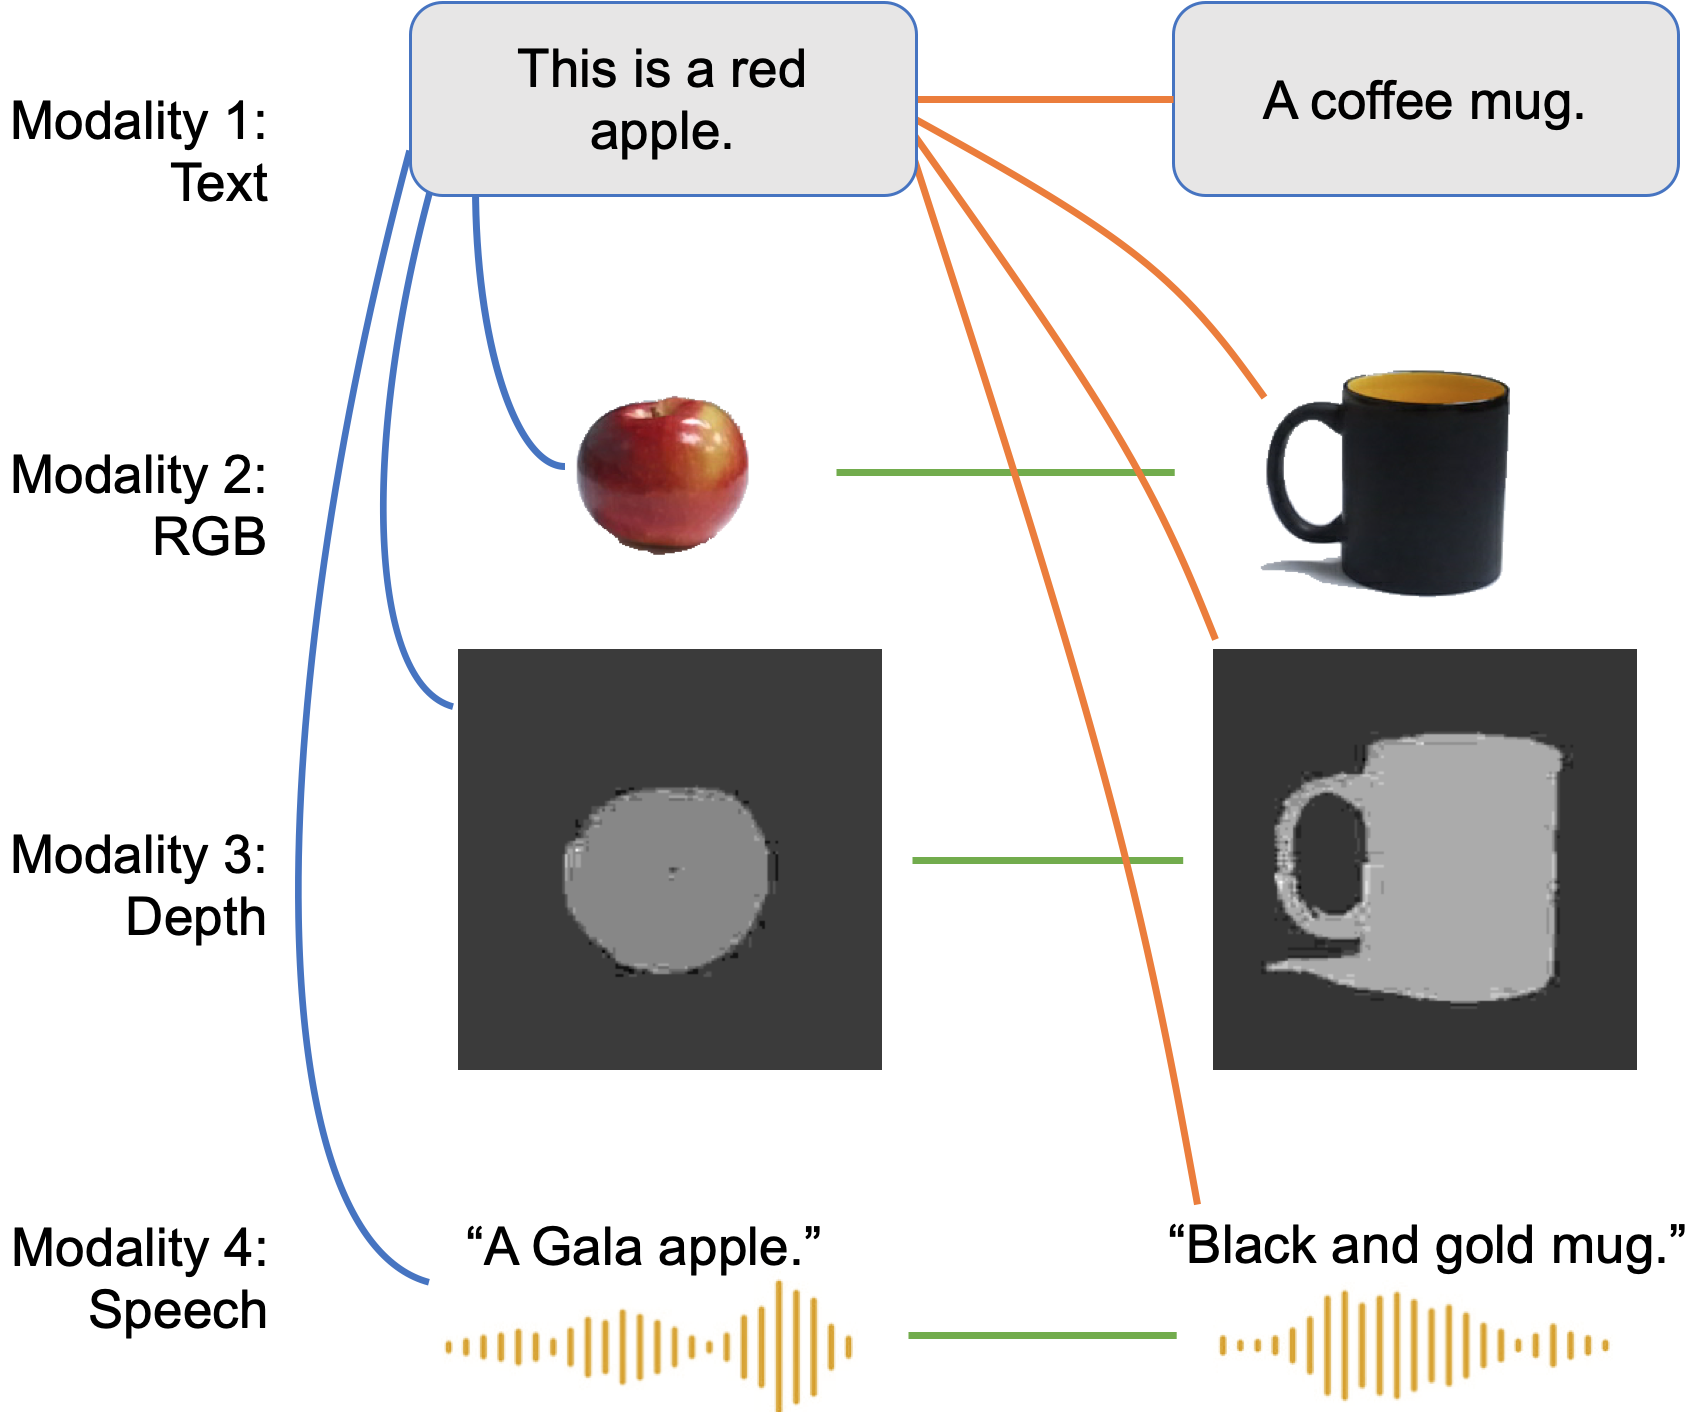
\includegraphics[width=.9\columnwidth]{Figures/4way-MMA.png}
% 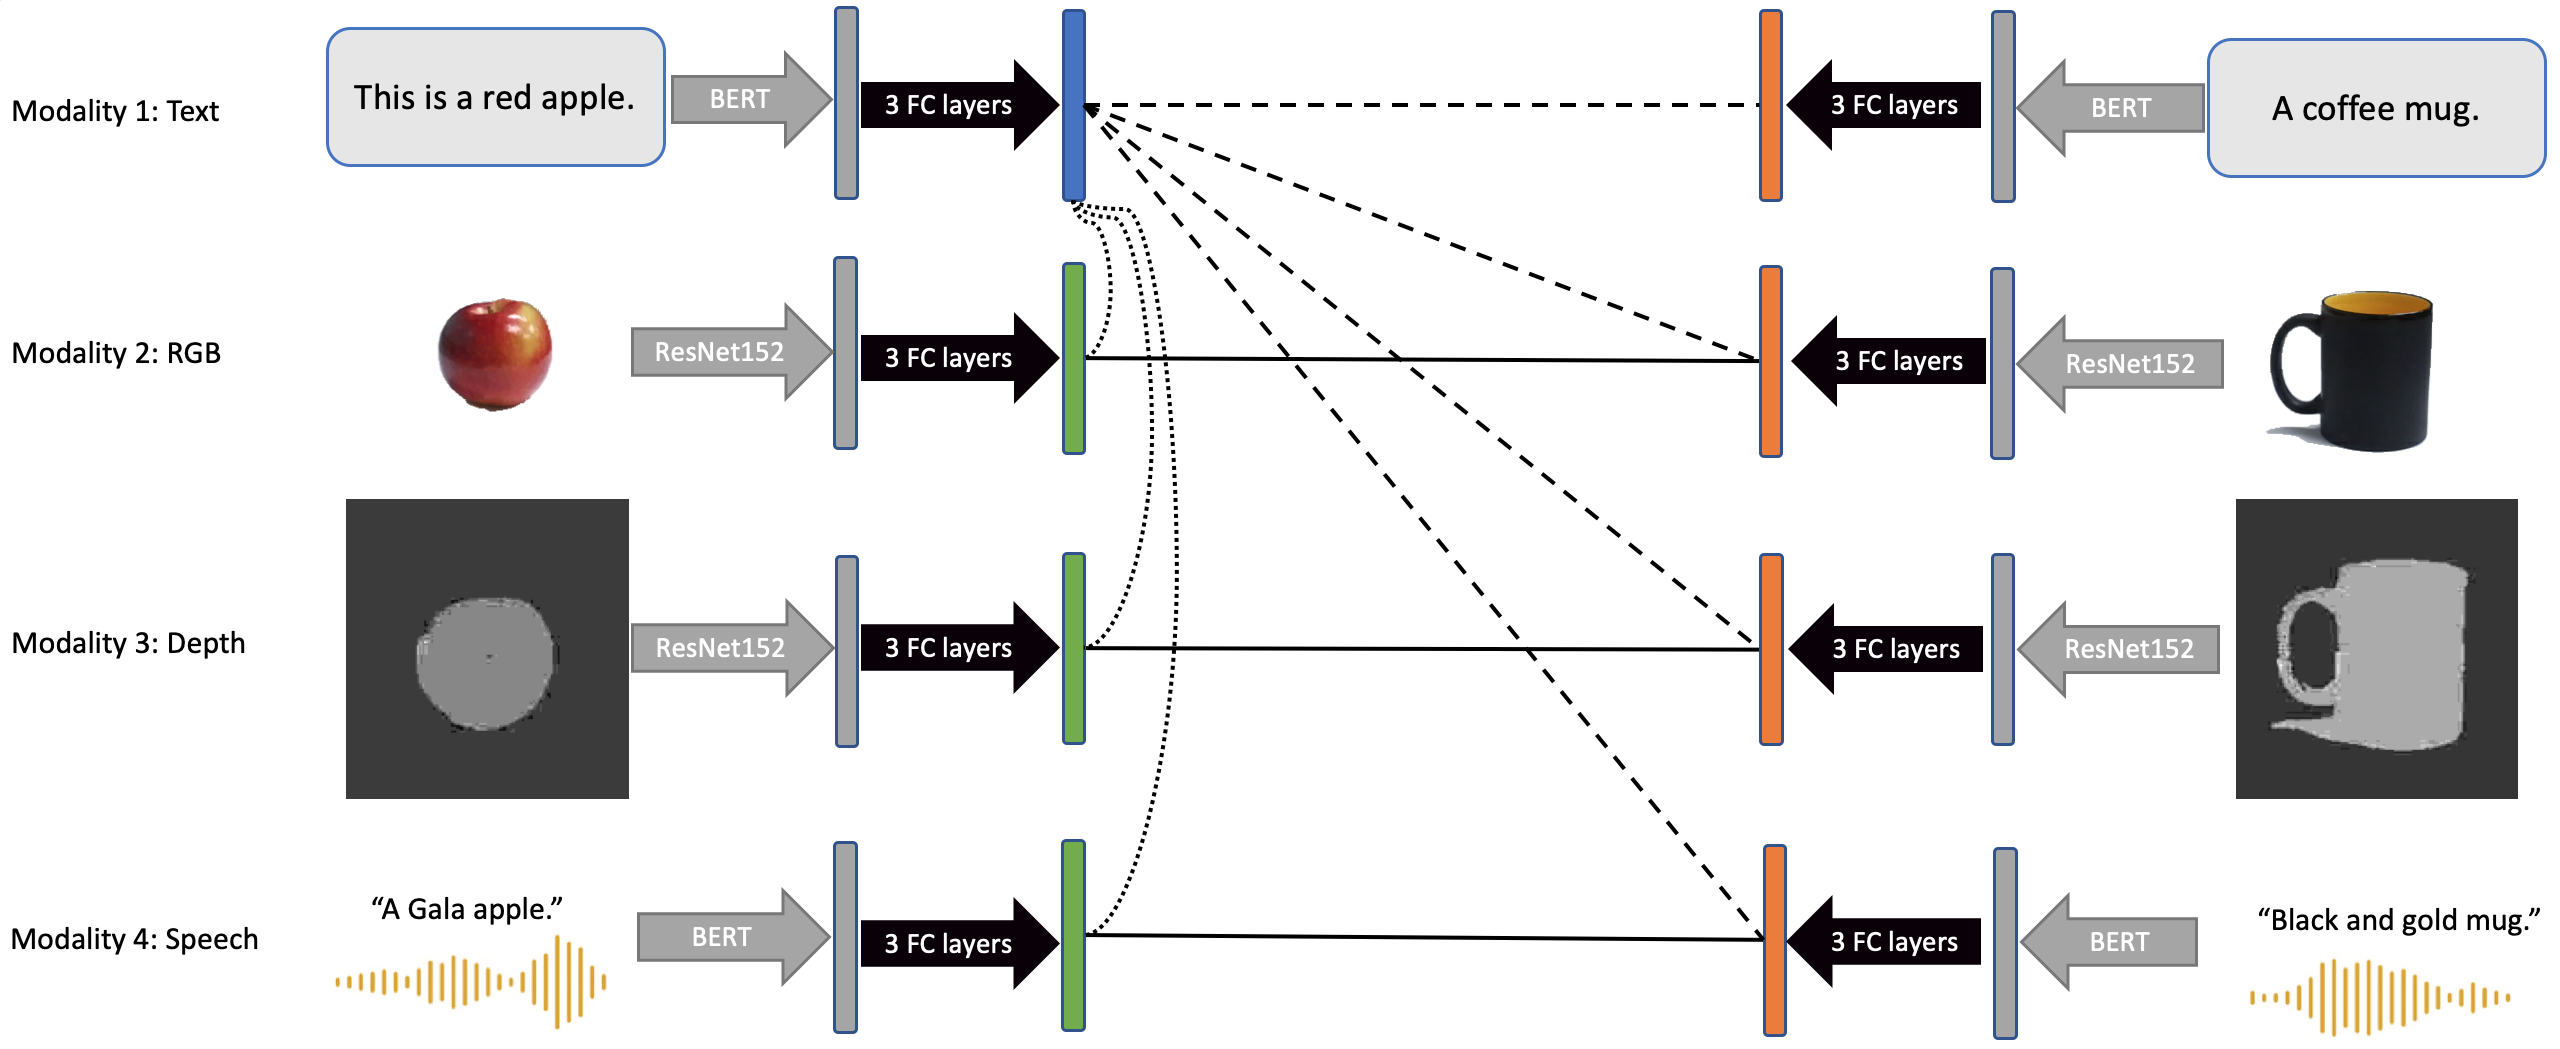
\includegraphics[width=2.1\columnwidth]{Figures/e-MMA.png}
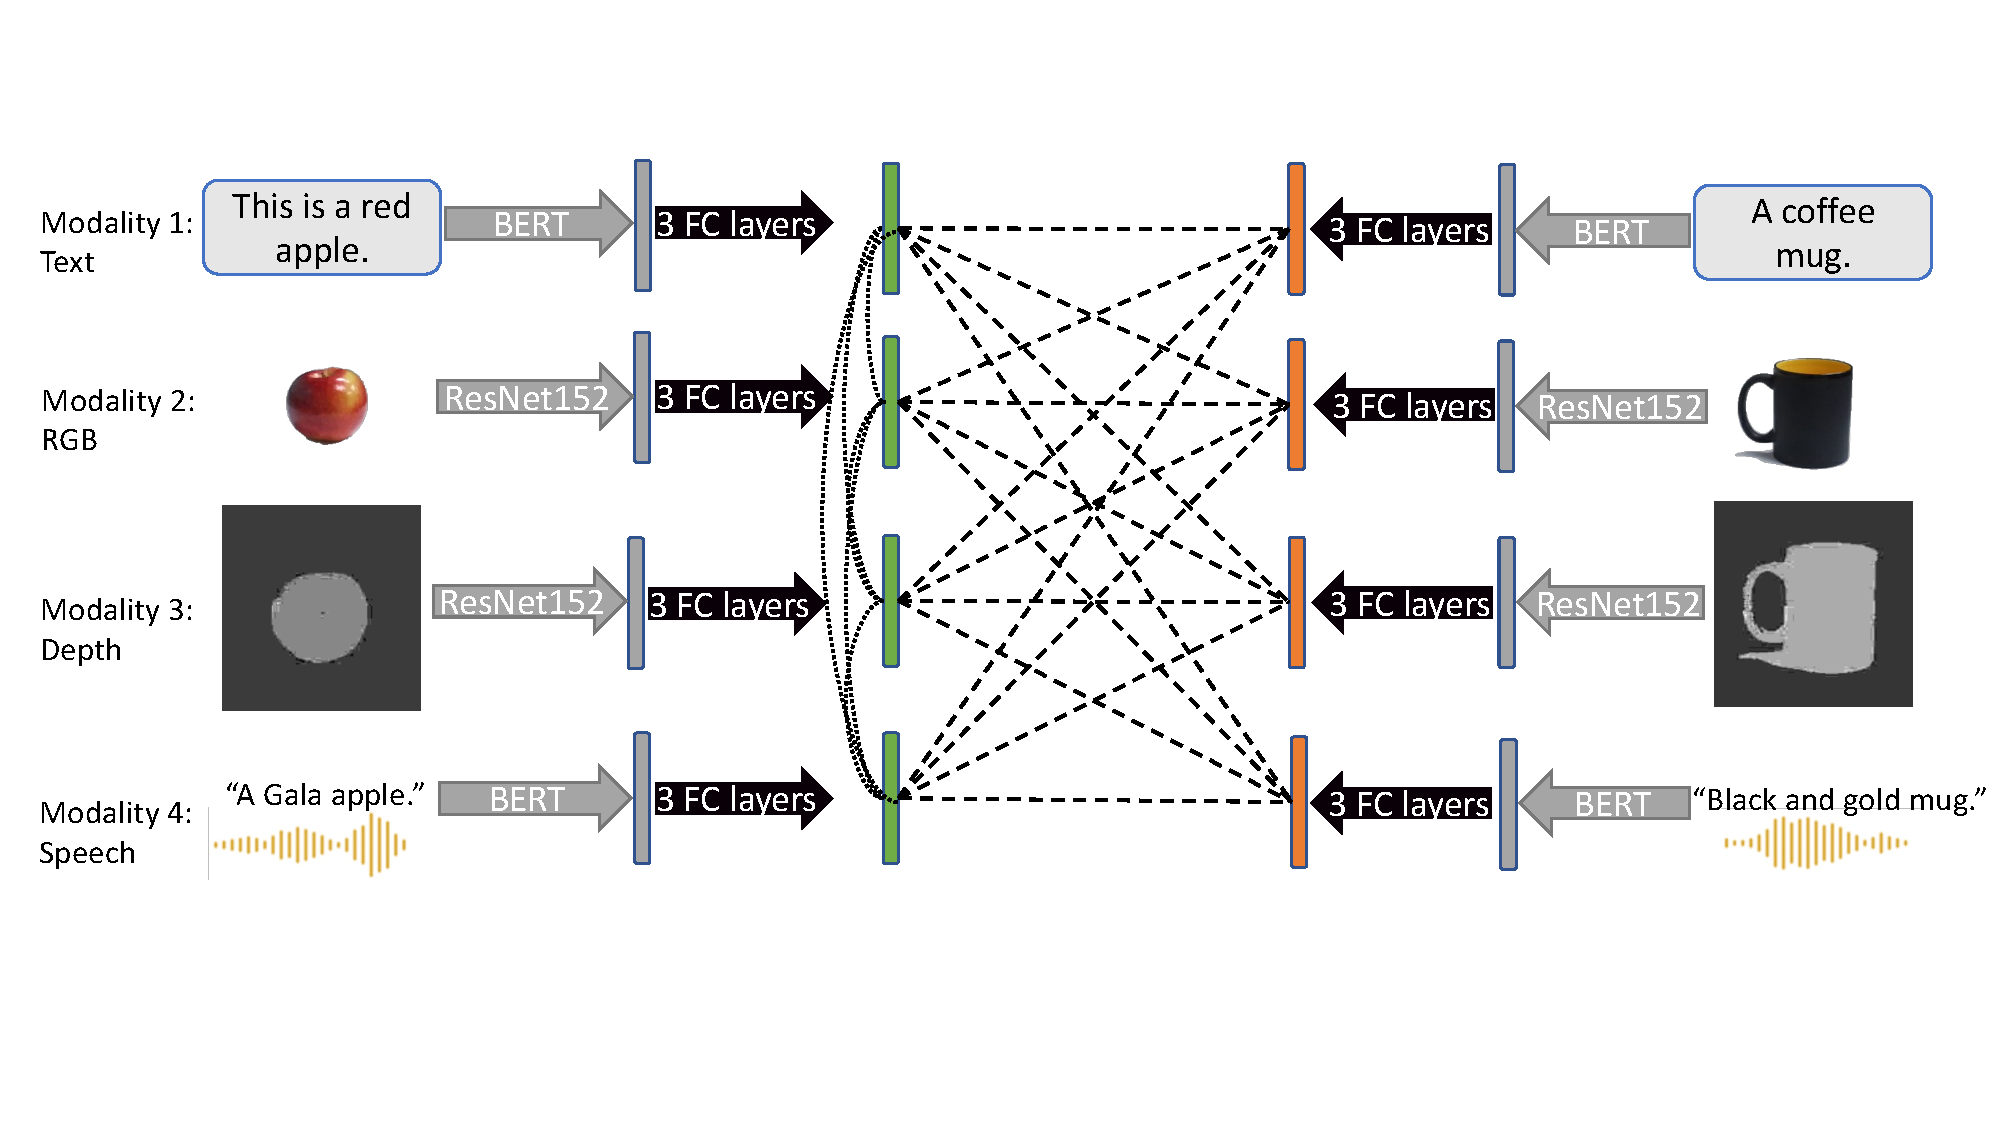
\includegraphics[width=1\columnwidth]{Figures/emma-loss-trimmed.pdf}
\caption{A high-level prototype of our approach and the distances used in the \geom{} loss with four modalities. Gray arrows indicate pre-trained models that are frozen (i.e. the parameters are fixed and are not trained). The black arrows show 3 fully connected layers with a ReLU activation function~\citep{relu2010} after the first two layers. These networks are trained.
Orange rectangles are negative embeddings and green rectangles are positive embeddings.
Dashed lines indicate distances to be maximized while dotted lines indicate distances to be minimized.%, and solid lines show the enforced margin.
}
\label{fig:emma-loss-trimmed}
\end{figure*}


Here, the generic \textit{dist} function is replaced with the specific $\cos(\cdot)$, and we omit the max notation for clarity by defining \cref{eq:aux-equation}:

\begin{equation}\label{eq:aux-equation}
    \begin{split}
        & g(x,y) = \max(\cos(x,y)-1 + \alpha, 0 ) \\
        & h(x,y) = \max(1- \cos(x,y), 0 ).
    \end{split}
\end{equation}


The first portion of the following equation maximizes all unique pairwise distances between modalities of positive and negative instances. The second portion minimizes the unique pairwise distances among the modalities of positive instances.

\begin{equation}\label{eq:objective-geom}
\begin{split}
    \mathcal{L} & = \sum_{m_1=1}^{M}  \sum_{m_2=1}^{M} g(z_{m_1}^{+}, z_{m_2}^{-})  + \sum_{m_1=1}^{M} \sum_{m_3=m_1+1}^{M} h(z_{m_1}^{+},z_{m_3}^{+})
    %  &= \sum_{i=1}^{M-1} \sum_{j=i+1}^{M} dist( z_{i}^{+} , z_{j}^{+}) - dist( z_{i}^{+} , z_{j}^{-}) - dist( z_{i}^{-} , z_{j}^{+}) - \sum_{i=1}^{M} dist( z_{i}^{+} , z_{i}^{-} ) \\
\end{split}    
\end{equation}
Our proposed \geom{} loss function in \cref{eq:objective-geom} can be rewritten as shown in \cref{eq:objective-geom-rewritten} by fully specifying the summations to better understand how our objective function can be reduced to well-known losses such as triplet loss and pairwise loss.

\begin{equation}\label{eq:objective-geom-rewritten}
\begin{split}
     \mathcal{L} &= \sum_{i=1}^{M-1} \sum_{j=i+1}^{M} h( z_{i}^{+} , z_{j}^{+})
     + g( z_{i}^{+} , z_{j}^{-}) + g( z_{i}^{-} , z_{j}^{+}) + \sum_{i=1}^{M} g( z_{i}^{+} , z_{i}^{-} ).
\end{split}
\end{equation}



If $M=2$ which means the number of modalities is 2, and we ignore the last two terms in the derived objective function, it results in the triplet loss method. 
If $M=2$, then our objective function reduces to the quadruplet loss method~\citep{tursun2021efficient,chen2017beyond} if we multiply the first term by 2, ignore the third term, and change the last summation to be up to $M-1$ (which results a single term). 
If $M=1$, only the last term remains in the loss function which is exactly the pairwise distance-based loss function.
This loss function can be seen as a contrastive loss usually used in the domain of self-supervised learning~\citep{chen2020simple}. However, our proposed loss function has two advantages over the traditional contrastive loss expressed in \cref{eq:contrastive-loss}. The first advantage is that our loss function does not loop over multiple positives and negatives in a large batch. Instead we sample only two objects (positive and negative) each of which have $M$ modalities which gives us $2M$ datapoints (or embeddings). Hence, our model can be trained using smaller batch sizes and reduces the number of negative samples we need. The second advantage is that this loss function can be used in a multimodal setting with an arbitrary number of modalities, and is not limited to a single data type (e.g. RGB images) which is the most common usage of contrastive loss.
% ~\citep{chen2020simple, NEURIPS2020_supervised_contrastive}.
Although our \geom{} is technically quadratic in terms of number of modalities, we observe that experimentally, training time increases only by 10 minutes with each additional modality.


Altogether, our proposed \geom{} function contains 
$3M^2-M/2$ terms: 
$M(M-1)/2$ anchor-to-positive distance minimizations and $M^2$ anchor-to-negative distance maximizations.
%, and $M(M-1)/2$ \textcolor{red}{optional} negative-to-negative distance minimizations.
%1 positive-to-negative anchor distance maximization.
It is noteworthy that our training procedure does not perform any stochastic dropout of modalities to obtain test-time robustness to missing modalities. Moreover, our approach does not need to compute the distance between all items in the batch, as opposed to \supcon{}.
% ~\citep{NEURIPS2020_supervised_contrastive}.

\paragraph{Combining Geometric and Cross-Entropy Losses}
\label{subsec:emma}

The main difference between \geom{} and \supcon{} is that in \geom{} we focus on the geometric interpretation of similarity using cosine distances, while in \supcon{}, cosine distances are used to compute a classification-based loss function similar to cross-entropy.
Both methods are valid and have some advantages that the other method does not offer. In \geom{}, the advantages are an intuitive learning objective in terms of distance, interpretability of the learned embedding space, and faster convergence. 
The advantage of \supcon{} is that it uses a classification objective which is aligned with the downstream task.

We propose to combine the \geom{} defined in \cref{eq:objective-geom} with \supcon{} defined in \cref{eq:supervised-contrastive}, and we refer to this approach as \ours{}, for extended multimodal alignment. The combination is done by taking the sum of the equations for \geom{} and \supcon{} which is shown in \cref{eq:emma}.
When


\begin{equation}\label{eq:emma}
\begin{split}
    \mathcal{L} =  \sum_{i \in I} \Biggr[ & \Bigr[ \sum_{j=1}^{M-1} \sum_{k=j+1}^{M} h( z_{i,j}^{+} , z_{i,k}^{+})
     + g( z_{i,j}^{+} , z_{i,k}^{-}) + g( z_{i,j}^{-} , z_{i,k}^{+}) + \sum_{j=1}^{M} g( z_{i,j}^{+} , z_{i,j}^{-} )\Bigr] + \\
     & \Bigr[ \sum_{m=1}^{M} \frac{-1}{|P(i,m)|}  \sum_{\beta \in P(i,m)} \log \frac{\exp (z_{i,m} \cdot z_{\beta} / \tau) }{\sum_{\gamma \in A(i,m)} \exp (z_{i,m} \cdot z_{\gamma} / \tau)} \Bigr] \Biggr], 
     \end{split}
\end{equation}
where $A(i,m)$ includes all items in the batch except for the $z_{i,m}$ itself and $P(i,m)$ includes all the modalities of all instances that have the same label as current instance excluding $z_{i,m}$ itself. 
In other words, the collection of embeddings indexed by $P(i,m)$ is $\{ \bigcup\limits_{r \neq m \in M} z_{i,r}, \bigcup\limits_{l \neq i \in I , y_i = y_l} \bigcup\limits_{m=1}^{M} z_{l,m} \} $.

% \todo[inline]{Which one do you prefer? The first one is my attempt at using almost the same terminology for both SupCon and Geometric method, while the second one is simply copying and pasting the two equations next to each other.}

% \begin{equation}\label{eq:emma-append}
%     \mathcal{L} = \Bigr[ \sum_{i=1}^{M-1} \sum_{j=i+1}^{M} -\cos( z_{i}^{+} , z_{j}^{+})
%      + \cos( z_{i}^{+} , z_{j}^{-}) + \cos( z_{i}^{-} , z_{j}^{+}) + \sum_{i=1}^{M} \cos( z_{i}^{+} , z_{i}^{-} ) \Bigr] + 
%      \Bigr[ \sum_{i \in I} \frac{-1}{|P(i)|} \sum_{p \in P(i)} \log \frac{\exp (z_i \cdot z_p / \tau) }{\sum_{a \in A(i)} \exp (z_i \cdot z_a / \tau)} \Bigr]
% \end{equation}

% 
% \begin{comment}
% 
% \begin{equation}\label{eq:emma}
%     % \mathcal{L} = \geom{} + \supcon{}
%     \ours{} = \geom{} + \supcon{}
% \end{equation}
% \end{comment}
% 
Compared to pure \supcon{}, combining these loss functions results in faster convergence and slightly improved performance when all modalities are available, and maintains improved performance when modalities are missing. Experimental results are presented in detail in \cref{sec:results}.

% We discuss the geometric interpretation of our method versus the classification interpretation of SupCon method and advantages of each. Finally, we show that combining \geom{} with \supcon{} is superior to either the \geom{} approach or \supcon{} alone.


\begin{comment}
\subsubsection{EMMA + Binary Classification}
\todokdinline{Should we remove this section?}

When batch size is 64, it performs worse than baseline (SupCon) and EMMA itself. The experiment for the batch size of 2 also performs worse than other versions of EMMA, except for when we drop text.

There is a slight chance that I have made a mistake in my implementation of binary cross-entropy loss. My guesses (in decreasing order of likelihood) are:

1. The inputs to the BCE loss are $sigmoid(\cos_{sim}(z_i,z_j))$ for all $i \neq j$ where i is over the positive modalities only, while j is over both positive and negative modalities. Maybe I should've used $1-\cos(pos_i, pos_j)$ for similar embeddings and $cos(pos_i, neg_j) -1$ for dissimilar embeddings instead; similar to how EMMA's geometric loss is structured.

2. Let's assume $\text{predicts} = \text{sigmoid}(\cos_{sim}(z_i,z_j))$. Their corresponding labels/targets are 1 if i and j are from positive modalities, and 0 if j is from the negative modalities. The way I used PyTorch's BCE is that I passed the predicts whose targets are 1 to BCE first, passed the predicts whose targets are 0 to BCE in the next step, and finally added the two together. In other words:


\begin{equation}
\begin{aligned}    
loss &= 0.0 \\
loss &= loss + BCE(\text{similar predicts, targets}=1) \\
loss &= loss + BCE(\text{dissimilar predicts, targets}=0)
\end{aligned}
\end{equation}

Adding temperature gives mixed results; when we have all the modalities during the test, adding temperature improves performance over not having a temperature, but is still slightly worse than other methods. When we drop the text modality, however, the performance goes down.
\end{comment}

\subsection{Network Architecture}
\label{sec:Model}

Transformers have become \textit{de facto} architectures in the natural language processing community and have shown great success across different tasks. Similar to~\citet{GoLD_UMBC}, we use BERT~\citep{devlin-etal-2019-bert} embeddings contained in the FLAIR library~\citep{akbik2019flair,akbik-etal-2019-pooled} to featurize textual input, and wav2vec2~\citep{wav2vec2} to extract audio embeddings from speech. Both of these encoders output a 3072-dimensional embedding vector which is generated by concatenating the last four hidden layers of their corresponding networks.
FLAIR has historically been used for different natural language processing tasks such as named entity recognition (NER) and part-of-speech tagging (PoS), and wav2veq2 has supported a a number of audio processing tasks, most notably automated speech recognition.
Both BERT~\citep{devlin-etal-2019-bert} and wav2vec2~\citep{wav2vec2} are self-supervised language models using transformers~\citep{vaswani2017attention}.
% 
To process images, we use ResNet152~\citep{He_resnet_2016} for both RGB and depth images which gives us a 2048-dimensional embedding vector. Depth images are colorized before passing to the ResNet152.

We then use different instantiations of the same multi-layer perceptron (MLP) consisting of 3 fully connected layers with ReLU activation~\citep{relu2010} to map each of these embeddings to a shared 1024-dimensional space where we can compute the distances between all embeddings. We note that these MLP networks are distinct and do not share any weights.




%===================================================================


\section{Experiments}
\label{sec:Experiments}

In this section we evaluate the quality of object retrieval models learned using the EMMA loss function. We first describe the dataset we use, then describe the metrics by which we evaluate performance, the setup of the experiments, and the baselines against which we compare. We end by presenting and analyzing results.

\subsection{Data}
\label{sec:Data}

We demonstrate the effectiveness of our approach on a recent publicly available multimodal dataset called GoLD~\citep{GoLD_UMBC}, which contains RGB images, depth images, written text descriptions, speech descriptions, and transcribed speech descriptions for 207 object instances across 47 object classes (see \cref{fig:emma-loss-trimmed}). There are a total of 16,500 spoken and 16,500 textual descriptions. The original GoLD paper uses raw RGB and depth images in which other objects are present in the background. We use a masked version of the images where the background is deleted (this masked version converges faster, however, masked and unmasked versions of the GoLD data converge to the same performance). Speech is converted to 16 Hz to match the wav2vec2 speech model.


\subsection{Setup}
% \label{sec:setupmetrics}
\label{sec:setup}
To evaluate our model we measure different performance metrics on a retrieval task where the model has to select an object from a set of objects given a language description. Only one of the objects corresponds to the description and the rest are from different object classes.
% (e.g., one apple among a set including a fork, a mug, a lemon, and a bell pepper).
% 
Similar to~\citet{NEURIPS2020_supervised_contrastive}, we use a stochastic gradient descent (SGD) optimizer with momentum~\citep{ruder2016overviewSGD} with a flexible learning rate starting at 0.05. 
% For the triplet loss experiments we use the Adam~\citep{kingma_adam_2015} optimizer with scheduling learning rate as suggested by the papers.
All models are trained for 200 epochs with a batch size of 64 on a Quadro RTX 8000 GPU. We used a temperature of $0.1$ for training the contrastive learning method described in \cref{sub:baseline-contrastive}, and a temperature of $0.07$ for training \supcon{} as described in \cref{sub:baseline-supcon}.


To evaluate the performance, we compute the distance between the given natural language description and 5 randomly selected objects (1 of which corresponds to the description, with the others from different object classes). We compute the distance between the language embedding and all available sensory modalities of all candidates as described in \cref{sub:ablations}. In case we have RGB and depth, we compute the distance between language embedding and all candidate RGB embeddings, and we compute the distance between the same language embedding and all candidate depth embeddings corresponding to the RGB embeddings. We then take average of these two distance matrices. Instead of choosing an empirical threshold beyond which objects are considered to be `referred to,' we choose the closest image embedding (average distance of RGB and/or depth from language) as the prediction.
In order to use cosine \textit{distance}, we have to subtract the cosine of the \textit{angle} between two embeddings (which represents similarity) from 1: that is, we compute $1 - \cos(e_1, e_2)$.

\subsection{Metrics}
\label{sec:metrics}
The best metric to capture the performance in such a scenario is mean reciprocal rank (MRR, \cref{eq:mrr} for $Q$ queries). For each query we predict the rank of all objects based on their distance from the language command, and then the inverse rank of the desired objects in all queries are averaged. For example, if the model predicts the desired object as the first rank, then MRR = $\frac{1}{1} = 1$ which means a perfect score, and if it predicts the correct object as the fourth rank among five objects, then MRR = $\frac{1}{4}=0.25$. 

\begin{equation} \label{eq:mrr}
    \mathrm{MRR}=\frac{1}{|Q|} \sum_{i=1}^{|Q|} \frac{1}{\operatorname{rank}_{i}}
\end{equation}

While MRR is more meaningful when it comes to ranking in retrieval tasks, in the real-world scenarios where a robot is asked to hand over an object, if it fails, it does not matter whether the correct object was ranked second or last and the whole system would be considered a failure.
Accuracy and micro F1 score
% (sklearn), flattened binary f1 score (sklearn), and F1 score 
are the same in this task, since for each prediction we either have a true positive and no false positives and no false negatives, or we have no true positives, one false positive and one false negative. MRR is a more informative metric because it captures the idea that having the correct object as the second choice should be considered better than having it as a last choice, while in accuracy the score is ``all or nothing''---either 0 or 1. Because our approach is designed to be robust to missing information across modalities, we also report MRR and accuracy for different combinations of modality dropouts. 


\subsection{Modality Ablation}
\label{sub:ablations}
% \todokdinline{Should I remove this section altogether or should I just mention that our method is equal or better in all cases except when we drop text? Or should I spend more time to come up with something so that we can perform better than baseline even in this case?}
We consider an experiment in which we incorporate RGB, depth, speech, and written language to train the model. The loss function requires no changes beyond adjusting the value of $M$ in \cref{eq:full-emma} according to the number of modalities available during training. Our goal is the non-trivial downstream prediction task: determining what objects are being referred to by arbitrary language from a small number of examples. When we consider only text, RGB, and depth, written language is used as the query modality, and we compute the distance of RGB and depth modalities from it and then average them. However, when speech is incorporated as an additional fourth sensory modality, we have three possible choices. First, we could compute the distance of RGB and depth from text and from speech which gives us 4 distance matrices, and then take average of these four. Second, we could treat speech in a similar way to RGB and depth: compute the distance of RGB, depth, and speech from text, and then take an average of three of them. Third, we could compute distances similarly to the first method, but add the distance between language and speech as well and then take the average of 5 distance matrices.

Of these, the first method is the most appropriate choice for a robust multimodal alignment approach. The second and third options are possible during training, but in real-world object retrieval scenarios, having only one form of language instructions is a reasonable scenario---people are not likely to \textit{both} speak about \textit{and} type in instructions for an agent. At test time, depending on which modalities are available to the model, we can use speech, text, or both to compute the distance of RGB and depth embeddings from the linguistic query, and then take the average.

There are total of nine possible cases of modality dropout and the corresponding distance computations. In all these cases \textit{t} represents text, \textit{s} represents speech, \textit{r} represents RGB, \textit{d} represents depth, and $K$ is the final distance---a matrix if there are multiple language queries and a vector if there is one query.
If we only have two modalities, we simply compute the distance between those two modalities; this corresponds to four of the cases; $K_{tr}$ when speech and depth are missing, $K_{sr}$ when text and depth are missing, $K_{td}$ when speech and RGB are missing, and $K_{sd}$ when text and RGB are missing. If we have three modalities, we need to take average of two distances. There are four cases with three modalities, $K_{trd} = \frac{K_{tr} + K_{td}}{2}$ when speech is missing, $K_{srd} = \frac{K_{sr} + K_{sd}}{2}$ when text is missing, 
and so on.
% $K_{tsr} = \frac{K_{tr} + K_{sr}}{2}$ when depth is missing, and $K_{tsd} = \frac{K_{td} + K_{sd}}{2}$ when RGB is missing. 
When we have all modalities available we take average of four distances, $K_{tsrd} = \frac{K_{tr}+ K_{td} +K_{sr} + K_{sd}}{4}$. 

% \Cref{eq:distance-matrix} shows all possible cases of modality dropout and the corresponding distance computations, where \textit{t} represents text, \textit{s} represents speech, \textit{r} represents RGB, \textit{d} represents depth, $K_{ij}$ for each pair of modalities is the distance of one instance in modality $i$ from all candidate instances in modality $j$, and $K$ is the final distance---a matrix if there are multiple queries and a vector if there is one query.

\begin{comment}
\begin{equation}
\label{eq:distance-matrix}
K = 
    \begin{cases} 
        K_{tr} & \text{speech and depth are missing} \\
        K_{sr} & \text{text and depth are missing} \\
        K_{td} & \text{speech and RGB are missing} \\
        K_{sd} & \text{text and RGB are missing} \\
        K_{trd} = \frac{K_{tr} + K_{td} }{2} & \text{speech is missing} \\
        K_{srd} = \frac{K_{sr} + K_{sd} }{2} & \text{text is missing} \\
        K_{tsr} = \frac{K_{tr} + K_{sr} }{2} & \text{depth is missing} \\
        K_{tsd} = \frac{K_{td} + K_{sd} }{2} & \text{RGB is missing} \\
        K_{tsrd} = \frac{K_{tr} + K_{td} + K_{sr} + K_{sd} }{4} & \text{o.w.} \\
    \end{cases}
\end{equation}
% \todo[inline]{equation \cref{eq:distance-matrix} takes a lot of space which suggests it's important. Either merge it in text or ...}
\end{comment}

\Cref{fig:result_graphs} shows the relative performance of \ours{} and \geom{} against state-of-the-art methods when different modalities are ablated.


\section{Results}
\label{sec:results}

In this section we provide quantitative and qualitative results by comparing our method against supervised contrastive learning~\citep{NEURIPS2020_supervised_contrastive} and na\"ive contrastive loss~\citep{chen2020simple}.
% We evaluate our EMMA loss function against the na\"ive triplet loss method. Our model significantly outperforms the triplet method across all epochs while it converges faster as shown in \cref{fig:epochs-mrr.srd}.
\Cref{table:quantitative} summarizes the performance of all models with different ablation metrics.
% \todo[inline]{Why do we call out triplet loss specifically? We evaluate against several baselines? I don't understand this section particularly}
To provide a better sense of the performance measure, consider a model that always ranks the correct object in the second place: Such a model would have an MRR of $1/2 = 0.5$.

\begin{table*}[tb]
    \centering
    \begin{subtable}[t]{1.00\textwidth}
    \centering
    \resizebox{1.0\textwidth}{!}{
    \begin{tabular}{|p{{2cm}}|p{{2cm}}|p{{2cm}}|p{{2cm}}|p{{2cm}}|p{{2cm}}|p{{2cm}}|p{{2cm}}|p{{2cm}}|p{{2cm}}|} 
 \hline 
Methods & speech/depth & speech/RGB & text/depth & text/RGB & text/speech/ \newline depth & text/speech/ \newline RGB & speech/RGB/ \newline depth & text/RGB/ \newline depth & all \\ 
 \hline 
Geometric & 76.82$\pm$0.34 & 78.34$\pm$0.29 & 89.64$\pm$0.38 & 91.13$\pm$0.73 & 89.21$\pm$0.45 & 90.95$\pm$0.83 & 79.37$\pm$0.29 & 92.29$\pm$0.51 & 92.14$\pm$0.45 \\ 
SupCon & \textbf{78.18}$\pm$0.58 & \textbf{79.69}$\pm$0.54 & 89.04$\pm$0.88 & 90.56$\pm$0.74 & 88.75$\pm$0.66 & 90.5$\pm$0.69 & \textbf{81.2}$\pm$0.39 & 91.96$\pm$0.42 & 92.03$\pm$0.7 \\ 
EMMA & 77.63$\pm$0.29 & 78.66$\pm$0.64 & \textbf{89.87}$\pm$0.5 & \textbf{91.26}$\pm$0.86 & \textbf{89.66}$\pm$0.36 & \textbf{90.97}$\pm$0.66 & 80.32$\pm$0.45 & \textbf{92.71}$\pm$0.5 & \textbf{92.72}$\pm$0.47 \\ 
Contrastive & 71.74$\pm$0.73 & 73.37$\pm$0.39 & 89.72$\pm$0.54 & 90.82$\pm$0.37 & 89.13$\pm$0.61 & 90.26$\pm$0.58 & 74.96$\pm$0.44 & 91.92$\pm$0.41 & 91.72$\pm$0.53 \\ 
\hline \end{tabular} 

    }
    \caption[]{Average and standard deviation of mean reciprocal rank (MRR) on a held-out test set. MRR is from $\frac{1}{\text{number of objects}}$\% to 100\%.
    In most cases \ours{} has a better MRR compared to other methods, and all methods have a higher MRR when text modality is present. This shows that text modality is a rich source of information compared to speech, and that \ours{} is strongly competitive with state of the art approaches even when relying on speech for the language signal.
    % \todocmi{Right? Correct}
    }
    \label{table:mrr}
    \end{subtable}
    \vskip\baselineskip
    \begin{subtable}[t]{1.00\textwidth}
    \centering
    \resizebox{1.0\textwidth}{!}{
    \begin{tabular}{|p{{2cm}}|p{{2cm}}|p{{2cm}}|p{{2cm}}|p{{2cm}}|p{{2cm}}|p{{2cm}}|p{{2cm}}|p{{2cm}}|p{{2cm}}|} 
 \hline 
Methods & speech/depth & speech/RGB & text/depth & text/RGB & text/speech/ \newline depth & text/speech/ \newline RGB & speech/RGB/ \newline depth & text/RGB/ \newline depth & all \\ 
 \hline 
Geometric & 61.95$\pm$0.55 & 64.34$\pm$0.53 & 82.03$\pm$0.57 & 84.6$\pm$1.1 & 81.08$\pm$0.81 & 84.0$\pm$1.4 & 65.84$\pm$0.63 & 86.41$\pm$0.83 & 85.94$\pm$0.74 \\ 
SupCon & \textbf{64.17}$\pm$0.92 & \textbf{66.52}$\pm$1.07 & 81.05$\pm$1.22 & 83.65$\pm$1.4 & 80.58$\pm$1.12 & 83.54$\pm$1.23 & \textbf{68.7}$\pm$0.66 & 86.06$\pm$1.21 & 85.82$\pm$1.29 \\ 
EMMA & 63.54$\pm$0.53 & 65.07$\pm$1.01 & 82.78$\pm$0.97 & \textbf{85.07}$\pm$1.42 & \textbf{82.16}$\pm$0.64 & \textbf{84.37}$\pm$1.23 & 67.69$\pm$0.81 & \textbf{87.38}$\pm$0.71 & \textbf{87.15}$\pm$0.72 \\ 
Contrastive & 54.82$\pm$1.4 & 57.27$\pm$0.64 & \textbf{82.88}$\pm$0.88 & 84.35$\pm$1.01 & 81.55$\pm$0.93 & 83.26$\pm$1.02 & 59.38$\pm$0.6 & 86.31$\pm$0.67 & 85.75$\pm$0.87 \\ 
\hline \end{tabular} 

    }
    \caption[]{Average and standard deviation of accuracy (Acc) on a held-out test set. Accuracy is from 0\% to 100\%.
    Although accuracy is a strictly less forgiving metric than MRR, these results demonstrate that \ours{} still outperforms existing approaches in the majority of cases. When we drop the text modality, the accuracy of the contrastive method is slightly better than random, while \ours{} is about 10\% more accurate than the contrastive method.
    }
    \label{table:acc}
    \end{subtable}
    \caption{Average and standard deviation of mean reciprocal rank (MRR) and accuracy (Acc) over 5 runs with 5 different random seeds on a held-out test set with different modalities ablated during testing. \Cref{table:mrr} shows MRR scores and \cref{table:acc} shows accuracy.
    % . These results represent performance when no modalities are ablated during training. 
     Higher is better for both metrics. For 5 objects, a random guess would have MRR of 0.33 and accuracy of 0.5, and the worst case performance would have MRR of 0.2 and accuracy of 0.0. The batch size is 64 and optimizer is SGD for all experiments. Column headers refer to modalities that are present at query time.
    % ---e.g., MRR \textit{sd} contains only speech and depth. 
    Bold numbers represent the best-performing method. \ours{} is either better than or very close to both state-of-the-art methods for most of the cases. We observe the same pattern in both MRR and accuracy except the fact that accuracy scores are lower than MRR.
    }
    \label{table:quantitative}
\end{table*}

\begin{comment}
\begin{table*}[tb]
    \centering
    \begin{subtable}[t]{1.00\textwidth}
    \centering
    \resizebox{.99\textwidth}{!}{
    \csvautotabular{Figures/unused/resultsMRR.csv}
    }
    \end{subtable}
    \vskip\baselineskip
    % \hfill
    \begin{subtable}[t]{1.00\textwidth}
    \centering
    \resizebox{.99\textwidth}{!}{
    \csvautotabular{Figures/unused/resultsACC.csv}
    }
    \end{subtable}
\end{table*}
\end{comment}


\begin{figure}
    \centering
    \begin{subfigure}[b]{0.49\textwidth}
        \centering
        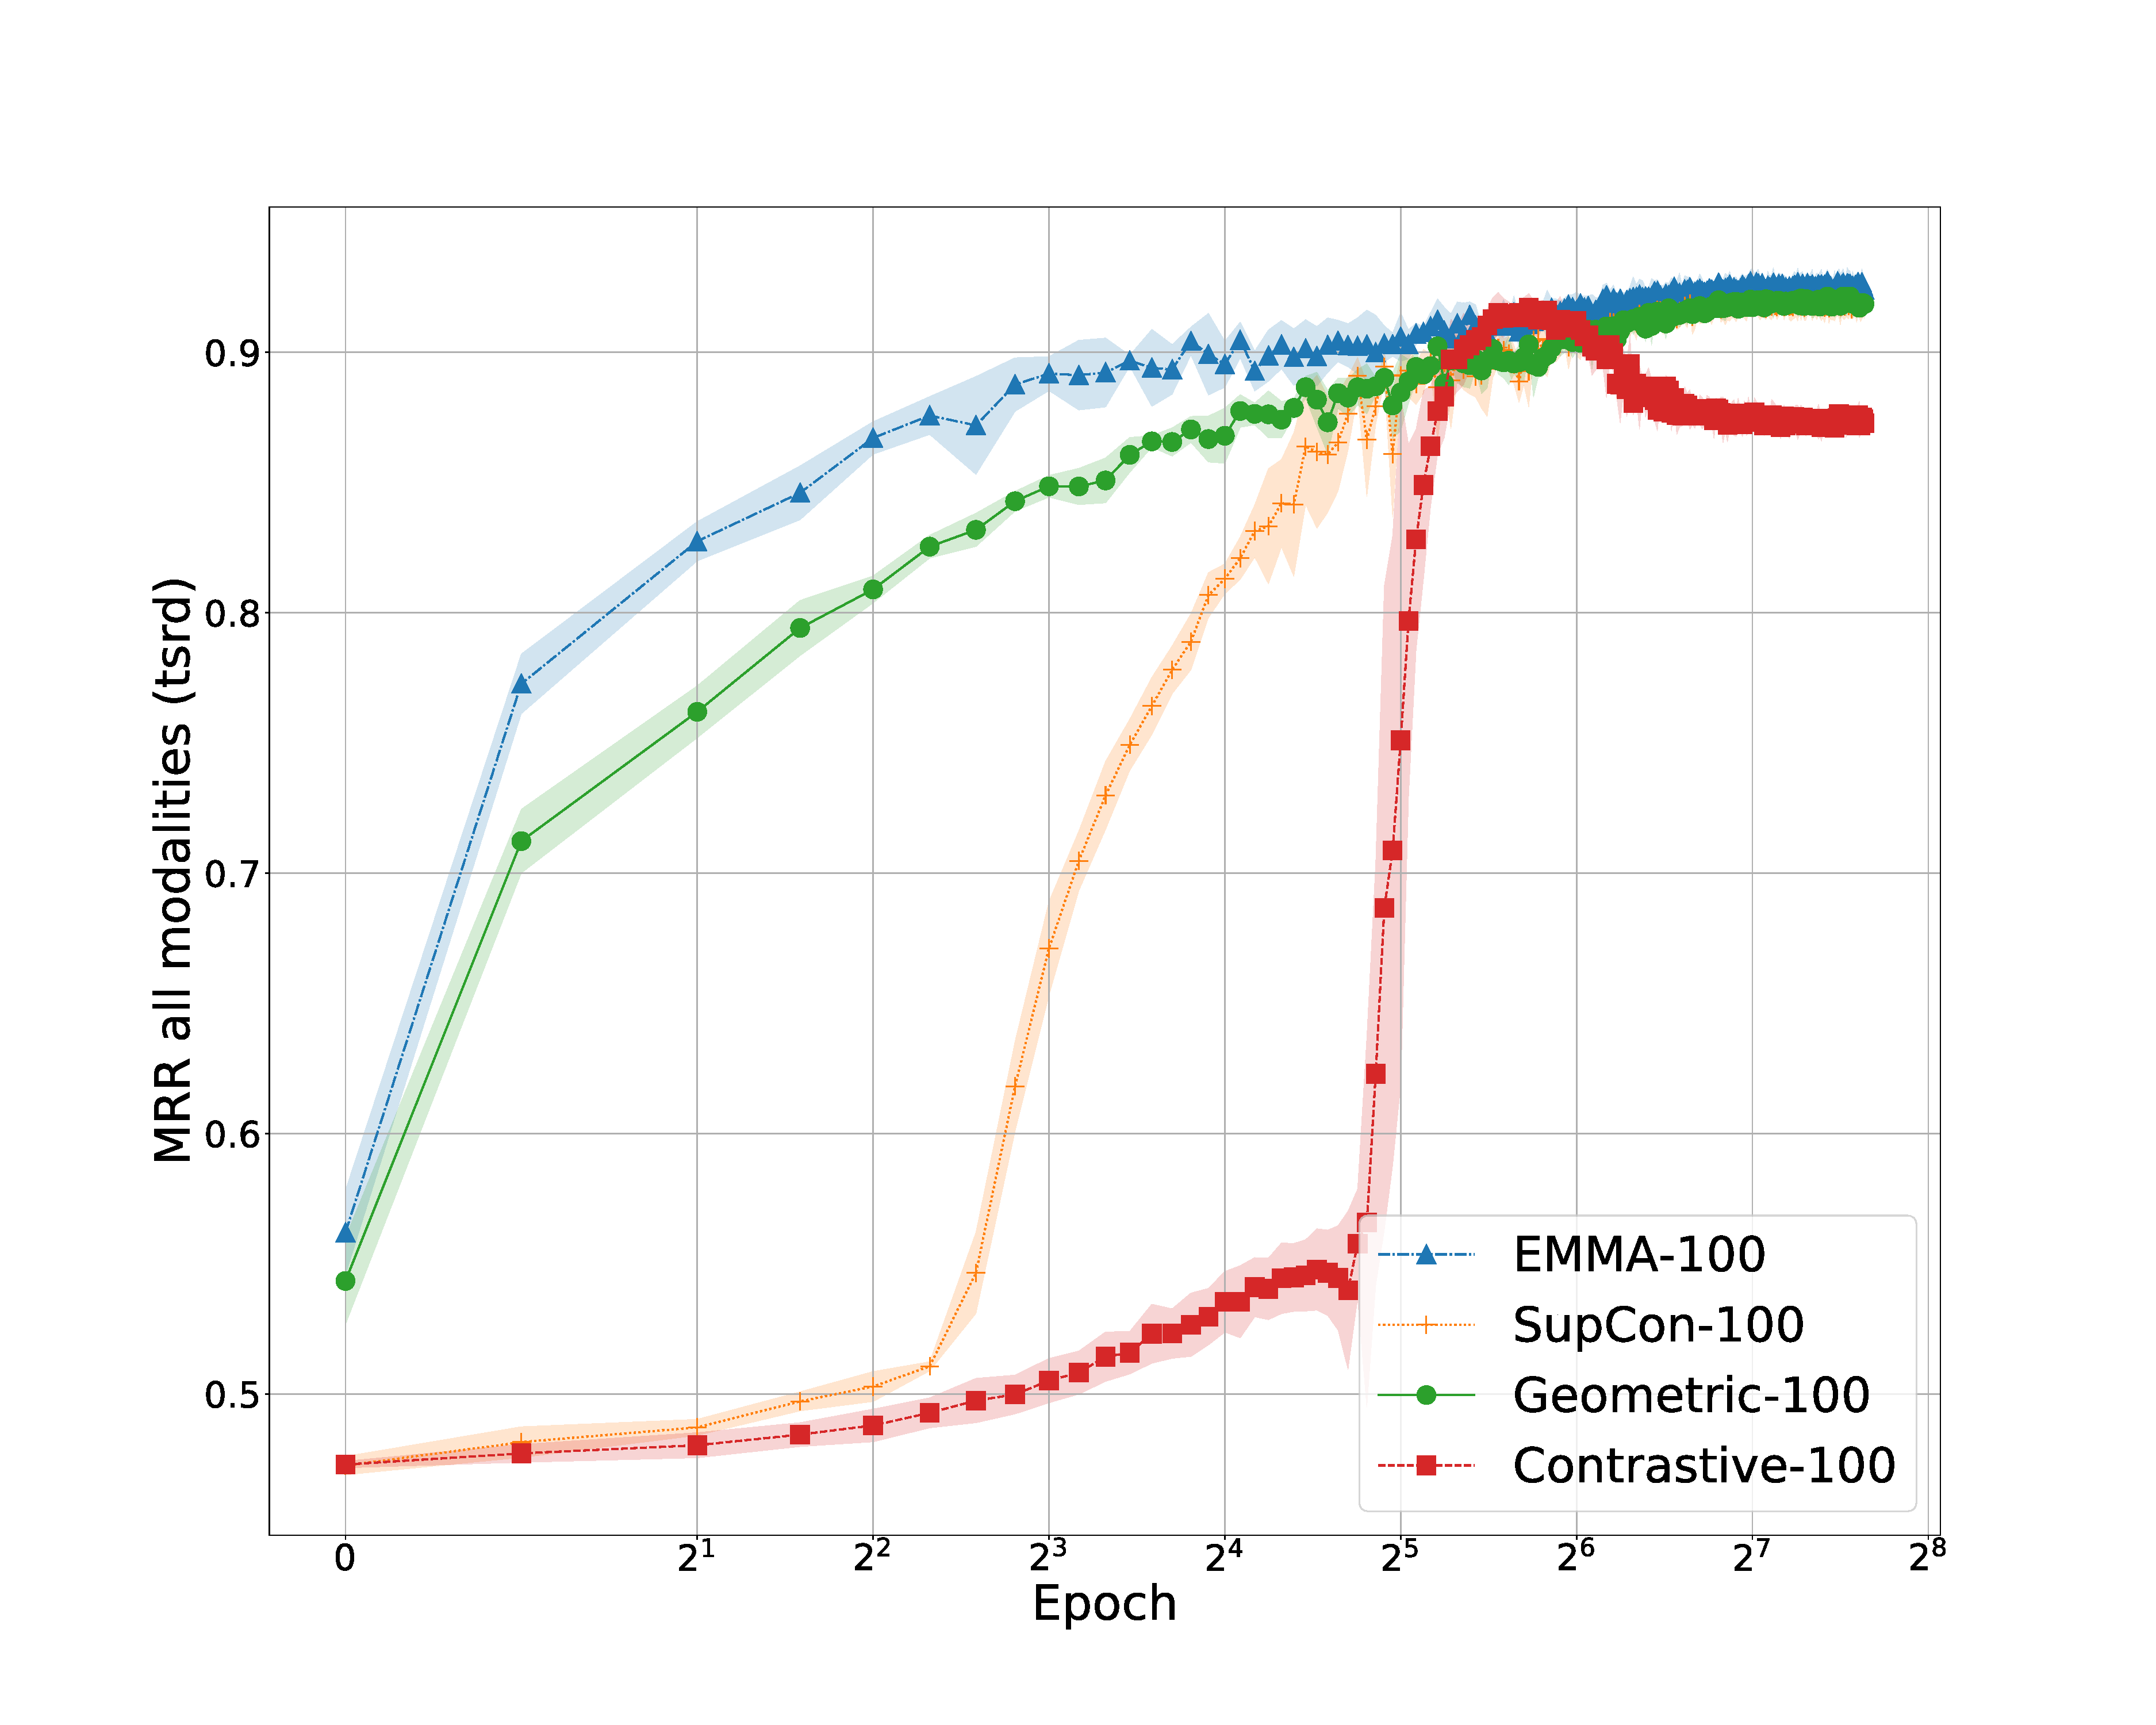
\includegraphics[width=\textwidth]{Figures/average-seeds-epochs-mrr_lard-trimmed.pdf}
        \caption[]{Mean Reciprocal Rank (MRR) on the held-out test set when all modalities are available.}    
        \label{fig:epochs-mrr.lard}
    \end{subfigure}
    \hfill
    \begin{subfigure}[b]{0.49\textwidth}  
        \centering 
        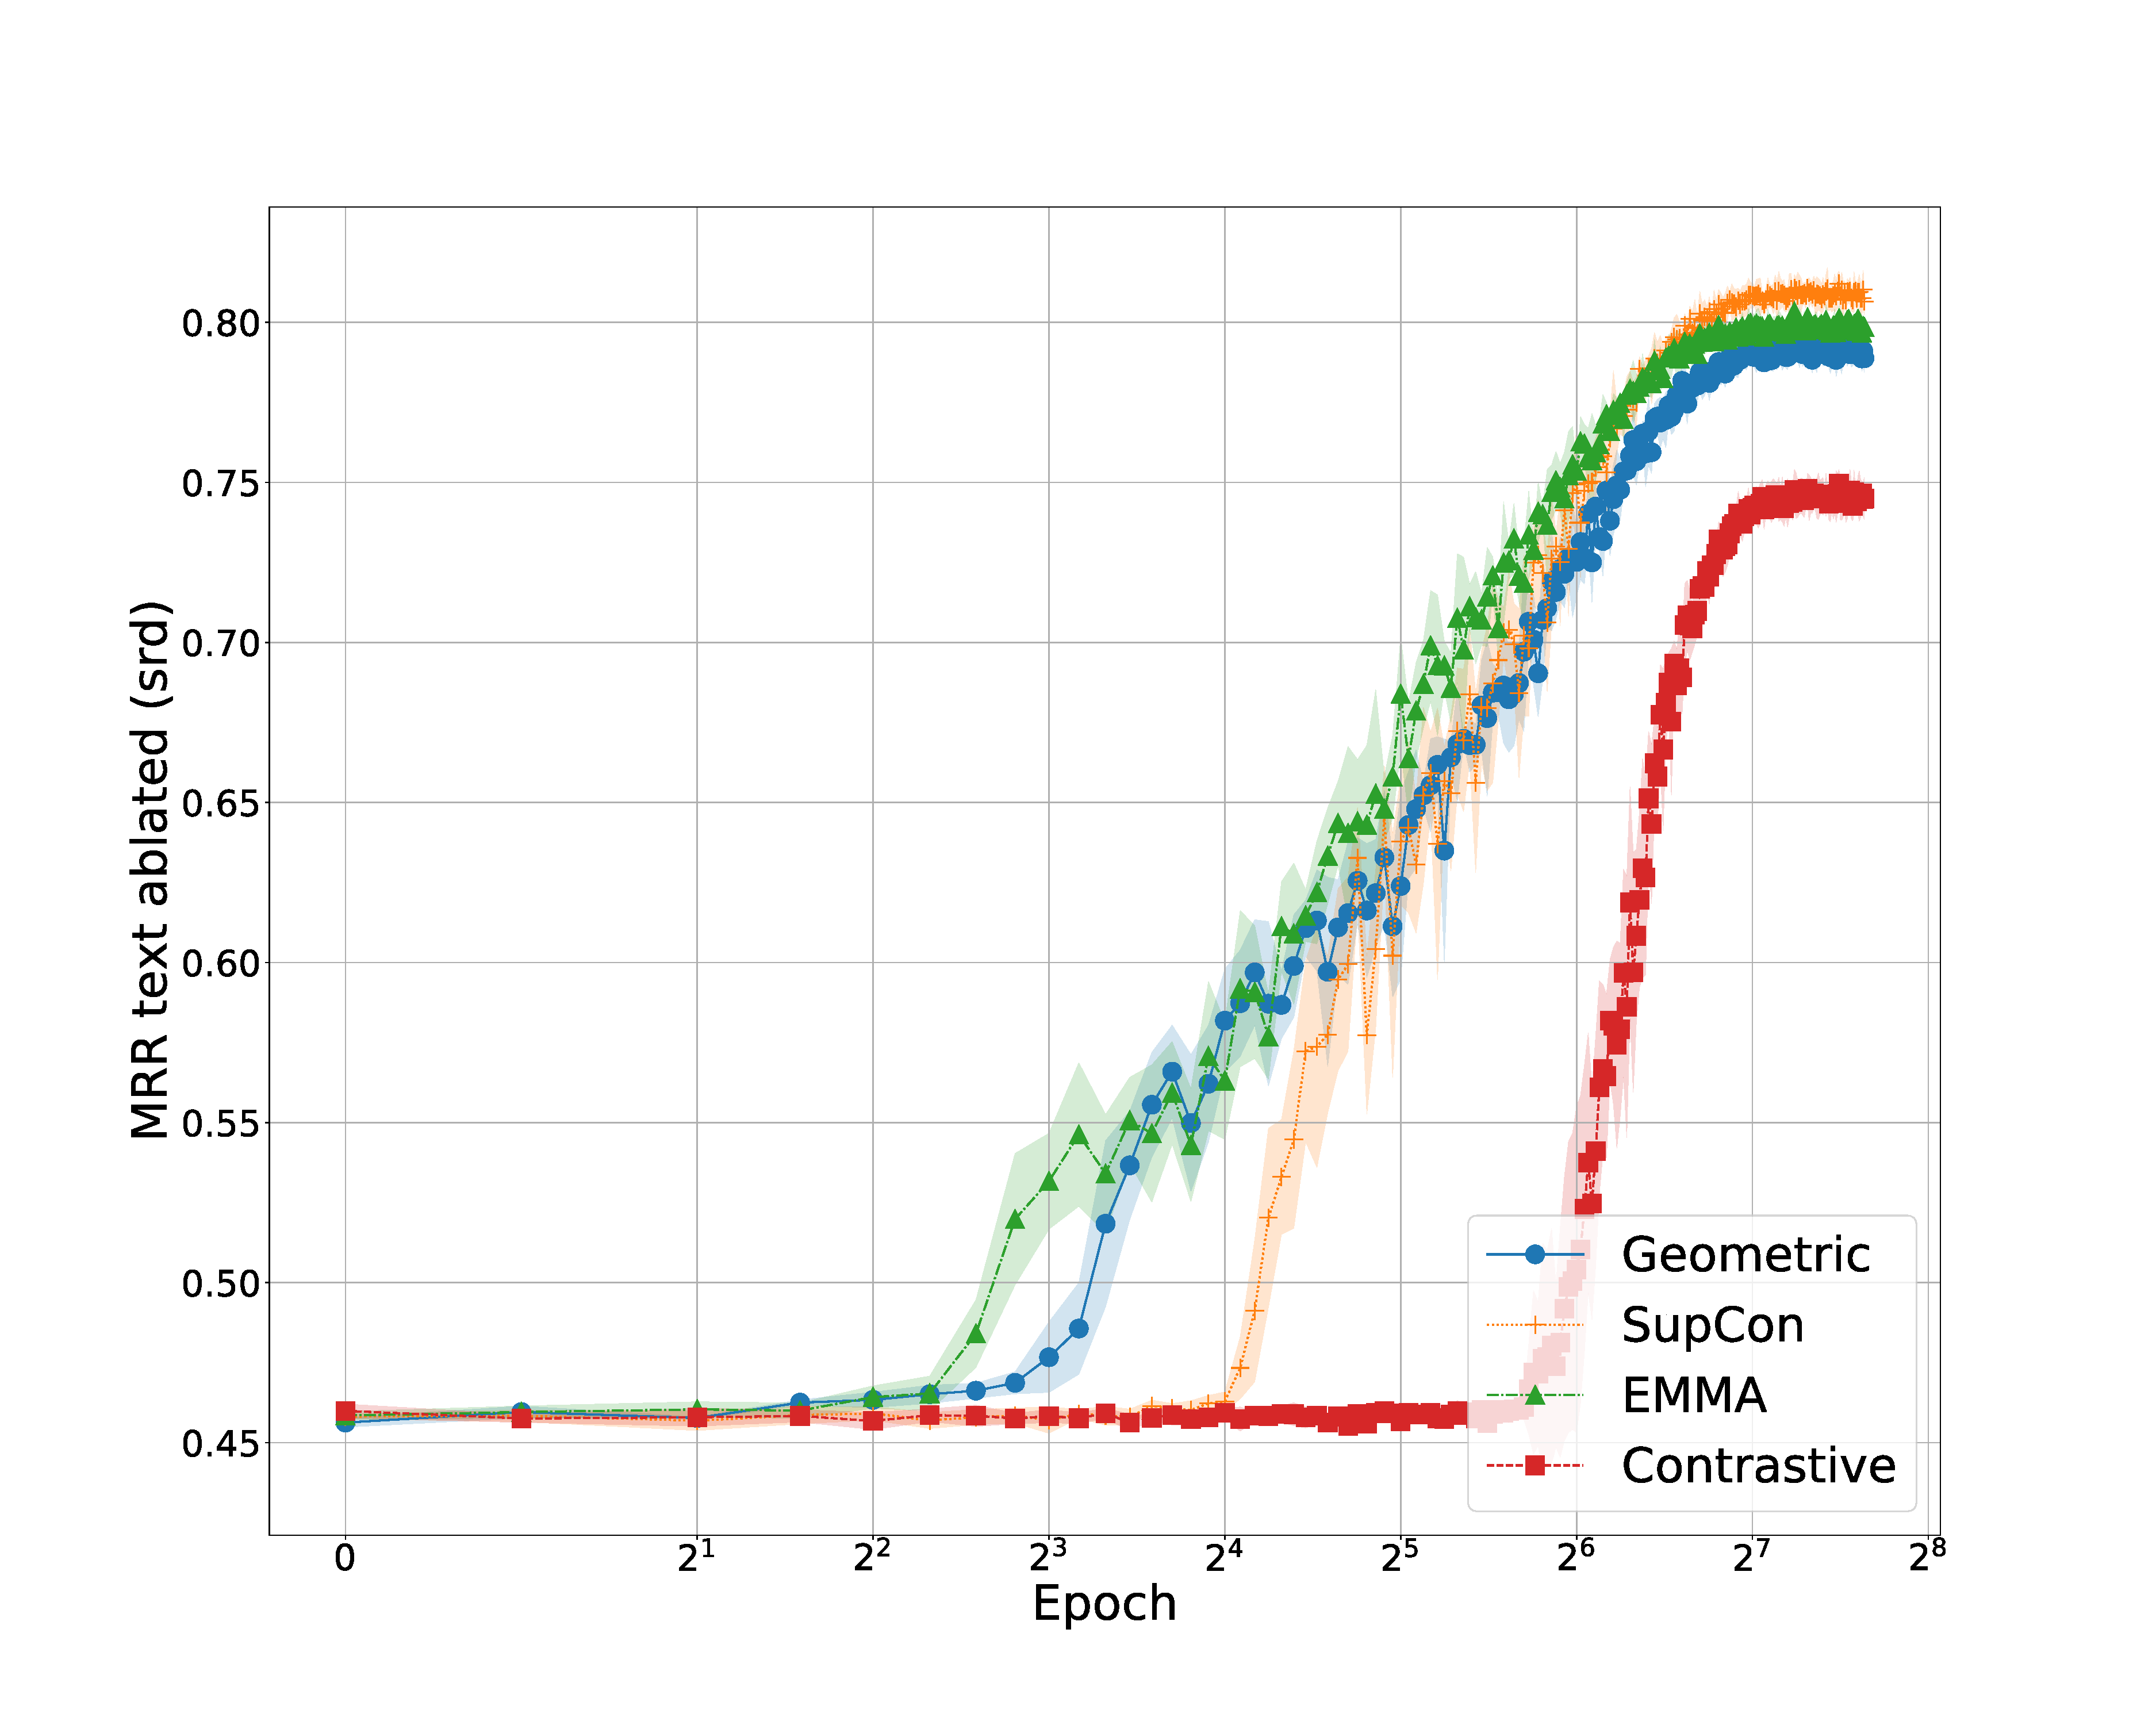
\includegraphics[width=\textwidth]{Figures/average-seeds-epochs-mrr_ard-trimmed.pdf}
        \caption[]{Mean Reciprocal Rank (MRR) on the held-out test set when the text modality is ablated.}
        \label{fig:epochs-mrr.srd}
    \end{subfigure}
    \vskip\baselineskip
    \begin{subfigure}[b]{0.49\textwidth}   
        \centering 
        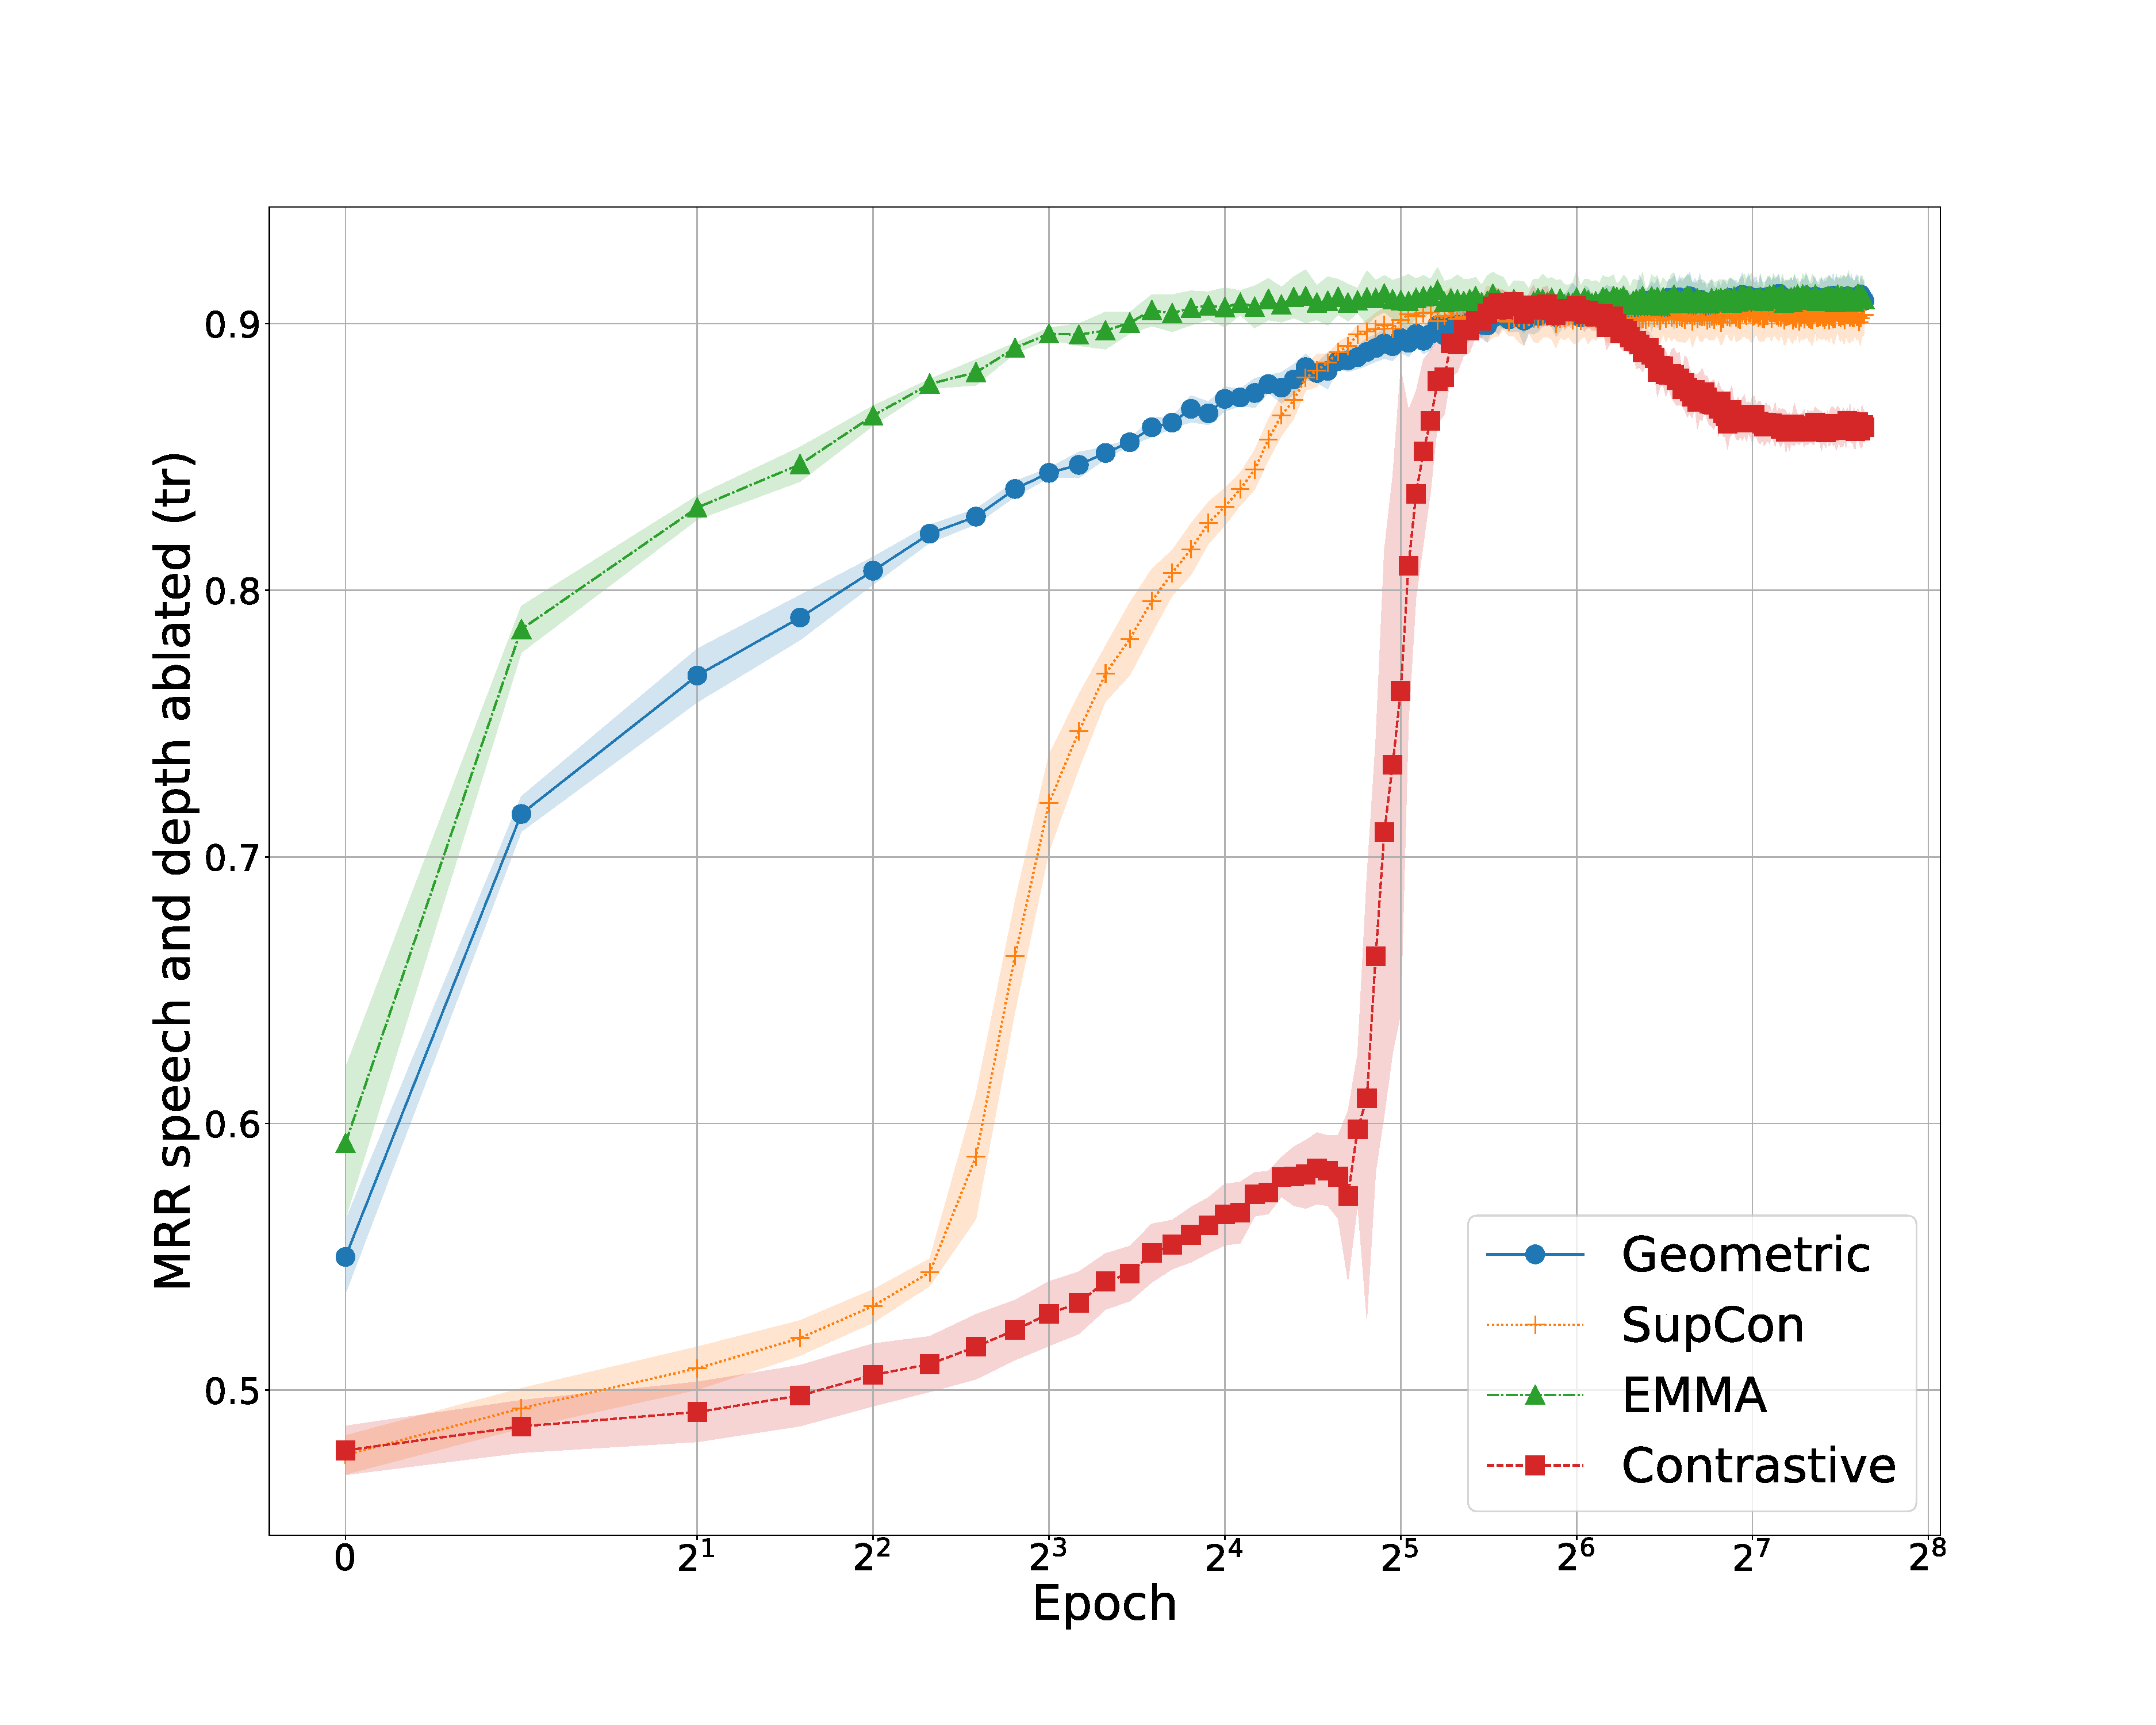
\includegraphics[width=\textwidth]{Figures/average-seeds-epochs-mrr_lr-trimmed.pdf}
        \caption[]{Mean Reciprocal Rank (MRR) on the held-out test set when speech and depth modalities are ablated.}    
        \label{fig:epochs-mrr.lr}
    \end{subfigure}
    \hfill
    \begin{subfigure}[b]{0.49\textwidth}   
        \centering 
        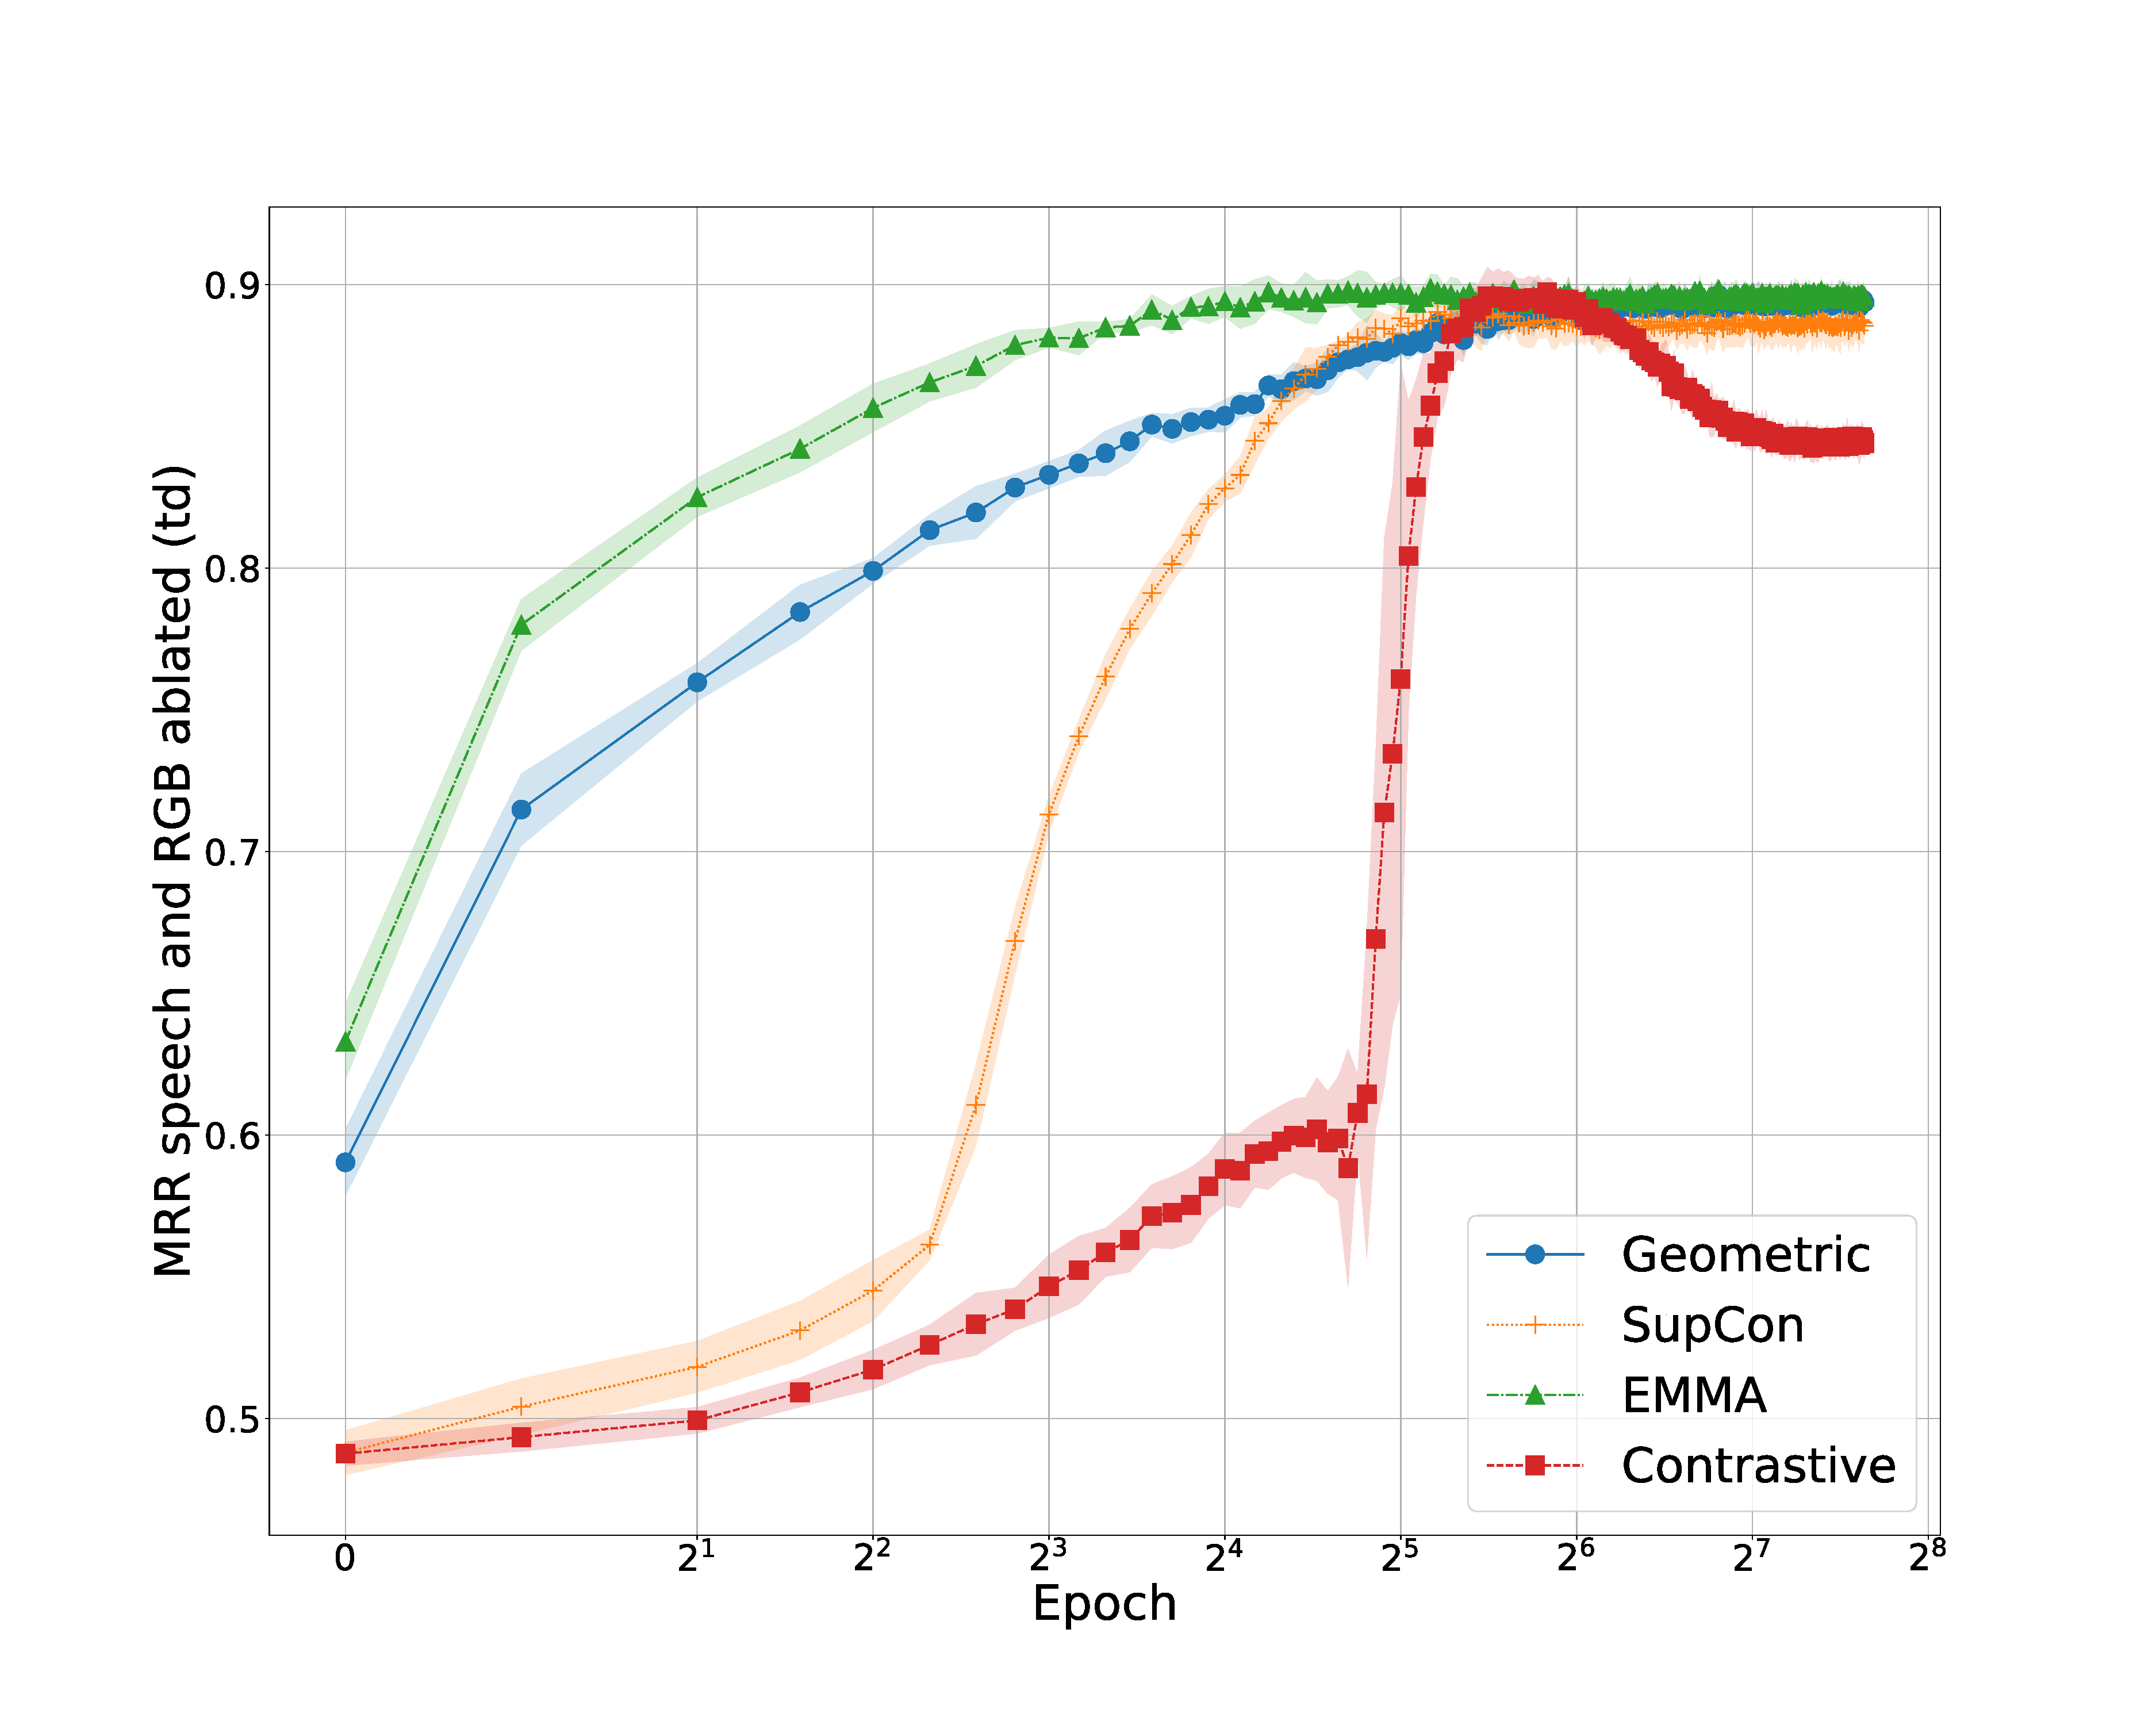
\includegraphics[width=\textwidth]{Figures/average-seeds-epochs-mrr_ld-trimmed.pdf}
        \caption[]{Mean Reciprocal Rank (MRR) on the held-out test set when speech and RGB modalities are dropped.}    
        \label{fig:epochs-mrr.ld}
    \end{subfigure}
    \caption[]
    {Mean Reciprocal Rank (MRR, \cref{eq:mrr}) on the held-out test set with the ablation of selected modalities, all averaged over 5 runs for the downstream task of object retrieval. Red is self-supervised contrastive learning which is prone to overfitting, orange is supervised contrastive learning, blue represents our proposed \geom{}, and green is our proposed \ours{} loss function. Higher is better. (a) shows the MRR when all modalities are available, (b) shows the MRR when text is removed at test time, (c) shows MRR when speech and depth are ablated, and (d) shows MRR when speech and RGB are removed. We train all models for 200 epochs.
    } 
    \label{fig:result_graphs}
\end{figure}
%     
% 
\Cref{fig:epochs-mrr.lard} Shows that \ours{} learns faster and results in a better performance compared to both \supcon{} and contrastive learning~\citep{chen2020simple} when trained using all modalities and with all modalities available during test. We observe that not only does contrastive loss learn more slowly, but that it is prone to overfitting; while this can be addressed with careful tuning of the learning process, an approach that is innately robust to overfitting without tuning is preferable.

When we drop the text modality (\cref{fig:epochs-mrr.srd}), we can see that the performance decreases from about 0.93 to about 0.82, showing that speech cannot completely replace text. In \cref{fig:3d-tsne} (see \cref{sec:Qualitative}), the alignment of shared embeddings for a randomly sampled set of classes is visualized for all four modalities under consideration, suggesting that the speech modality is not aligned as well as the text modality. For this reason, when we drop text and use speech as the main query, the performance decreases. This supports our hypothesis that a geometric alignment of the latent space is crucial to a good performance for object retrieval and multimodal understanding.

In \cref{fig:epochs-mrr.srd}, we observe that when speech is used as the query and the text modality is ablated, the \supcon{} baseline works slightly better than \ours{}, although \ours{} still learns faster. The reason is that \supcon{} optimizes for the classification task, and since the speech modality is less well aligned, using \geom{} makes the downstream task more difficult by trying to pull and push similar and dissimilar data points, respectively. Future research will consider strategies to align more chaotic modalities.
% We also observe that speech has a higher variance compared to text, and a na\"ive contrastive learning method cannot take advantage of text modality to reduce this variance. While the other two methods leverage text modality to align speech better.

There is very little gap in performance when depth or RGB are dropped in \cref{fig:epochs-mrr.lr,fig:epochs-mrr.ld} compared to when we have all modalities in \cref{fig:epochs-mrr.lard}, showing that our model is robust when RGB or depth sensors fail. Also, when depth is dropped in \cref{fig:epochs-mrr.lr}, performance decreases less compared to when RGB is dropped in \cref{fig:epochs-mrr.ld}. This suggests that depth is less informative when compared to RGB, which is consistent with existing vision research results. 

% \todocmi{Main remaining task is to sort out figures. They should all have meaningful y axis labels and essentially no whitespace surrounding them.}

\paragraph{Qualitative Results}
\label{sec:Qualitative}
In order to help visualize the performance of learned embeddings, we consider projections of a randomly selected subset of classes of the high-dimensional learned embeddings into a 3-dimensional space using t-SNE~\citep{van2008tsne}, a dimensionality reduction technique to visualize high-dimensional data. T-SNE creates a probability distribution over pairs of high-dimensional data where similar pairs have a higher probability and dissimilar pairs have a lower probability. A similar probability distribution is also defined over pairs of data in the lower dimension (either 2D or 3D), and T-SNE minimizes the KL divergence between these two probability distributions.
% \textcolor{red}{\dots}\todo{explanation}. 
% \Cref{fig:2d-tsne} shows the projection of all test embeddings from all different modalities in a 2D space. As shown in the graph, instances of the same class but different modality are mapped to almost the same locations and are closer to each other.
\Cref{fig:3d-tsne} shows the projection onto 3D space to give a better view of the location of embeddings. Although these projections are not perfect, combined with the quantitative results, they demonstrate that our model is learning to map instances of the same class closer to each other regardless of their modalities. Interestingly, toothbrush and toothpaste are mapped almost on top of each other in the text modality showing semantic and syntax similarity. However, in the RGB and depth modality they are close but not on top of each other since they do not look the same. Also, we can see that apple and lemon are mapped close to each other in all modalities which suggests that our proposed \ours{} learns some notion of the concept of fruits. These qualitative results show that our propose \geom{} and \ours{} have an interpretable latent space.

\begin{figure*}[h]
\centering
% 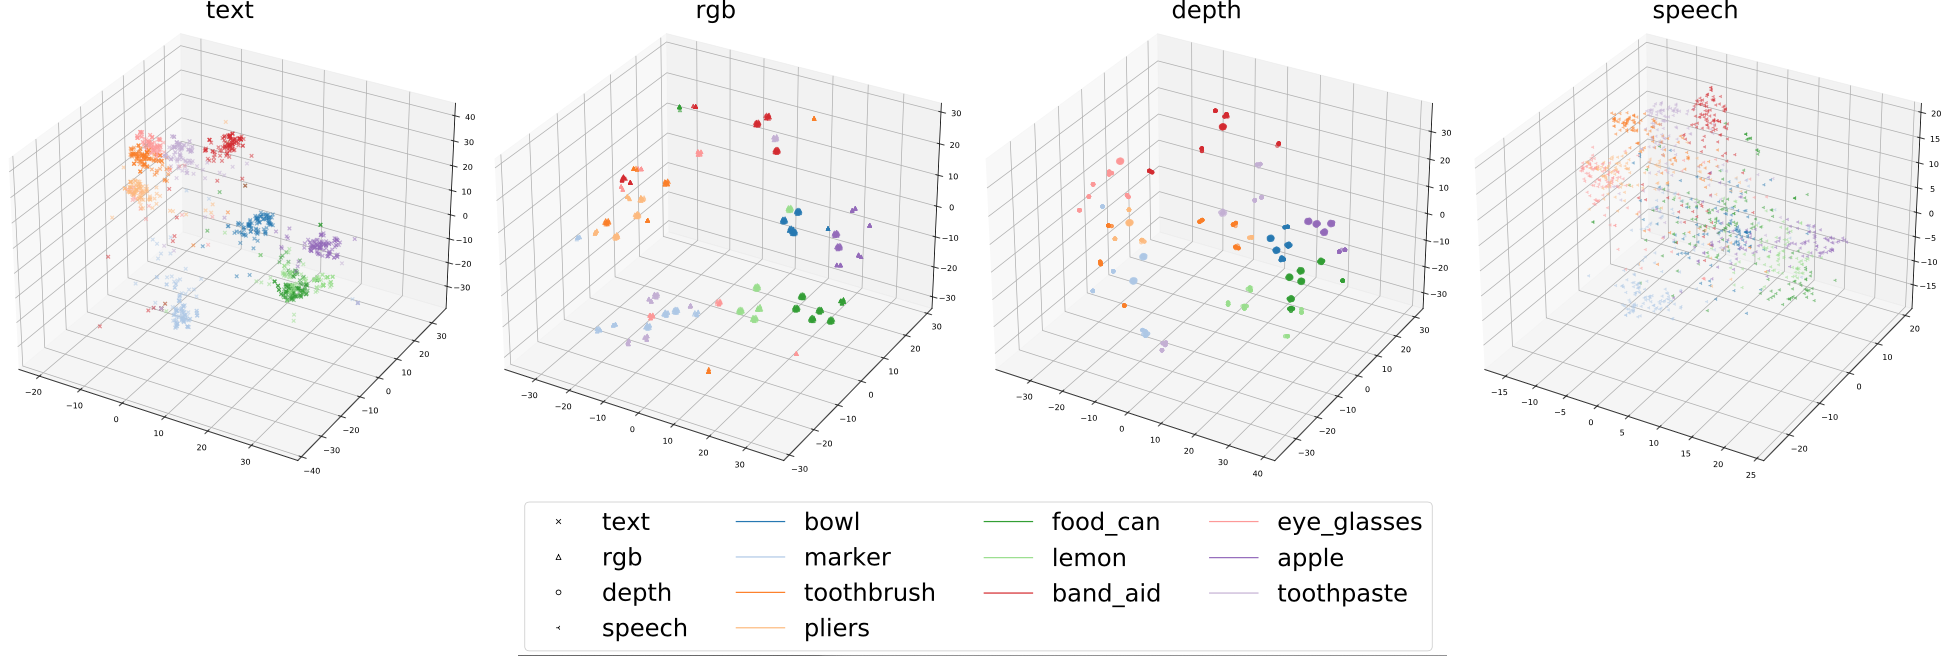
\includegraphics[width=1.99\columnwidth]{Figures/3D-tsne-4M-eMMA-cosine-submodalities-text-anchor-gold-no_neg_sampling-1024-sbs.png}
% 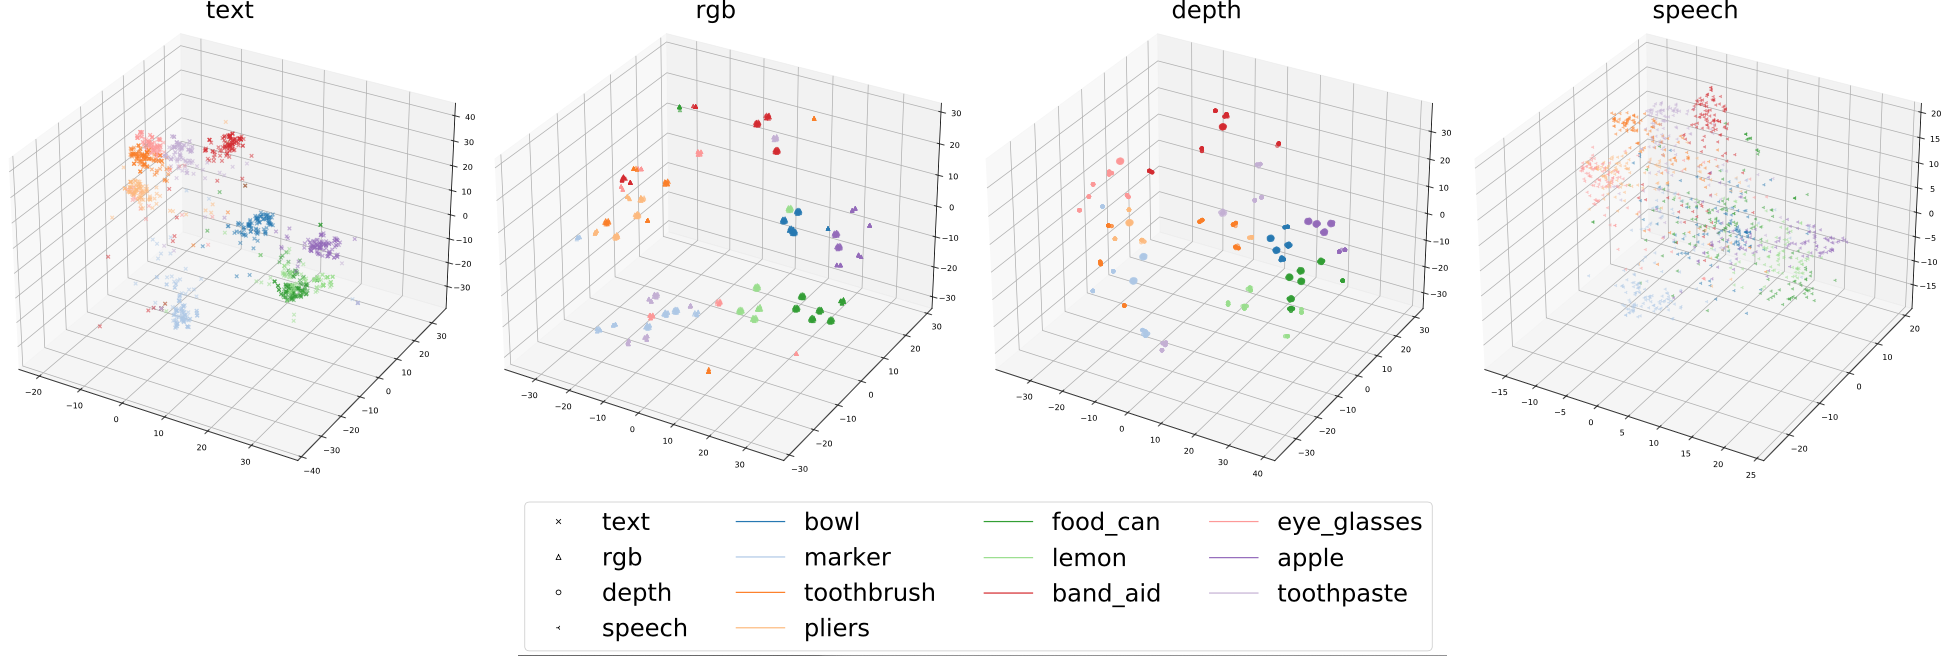
\includegraphics[width=1\columnwidth]{Figures/3D-tsne-4M-eMMA-cosine-submodalities-text-anchor-gold-no_neg_sampling-1024-sbs.png}
% 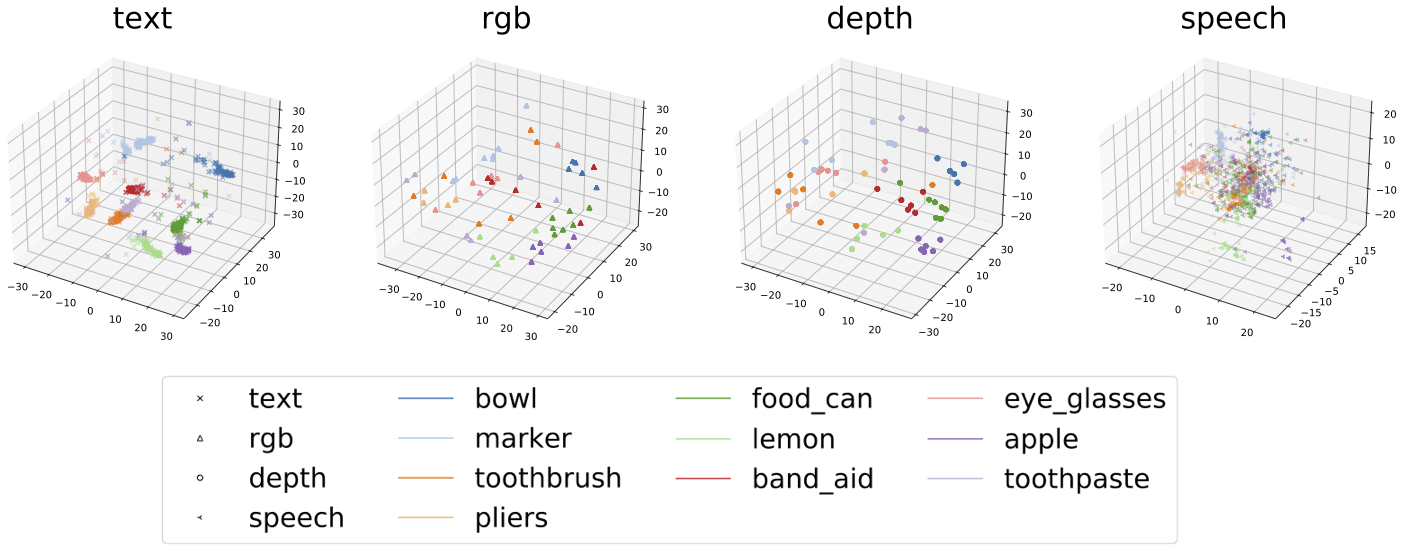
\includegraphics[width=.99\columnwidth]{Figures/3D-tsne-exp-supcon-emma-lard-64-relu-SGD-0.001-unique_objects-gold-no_neg_sampling-1024-sbs-trimmed.png}
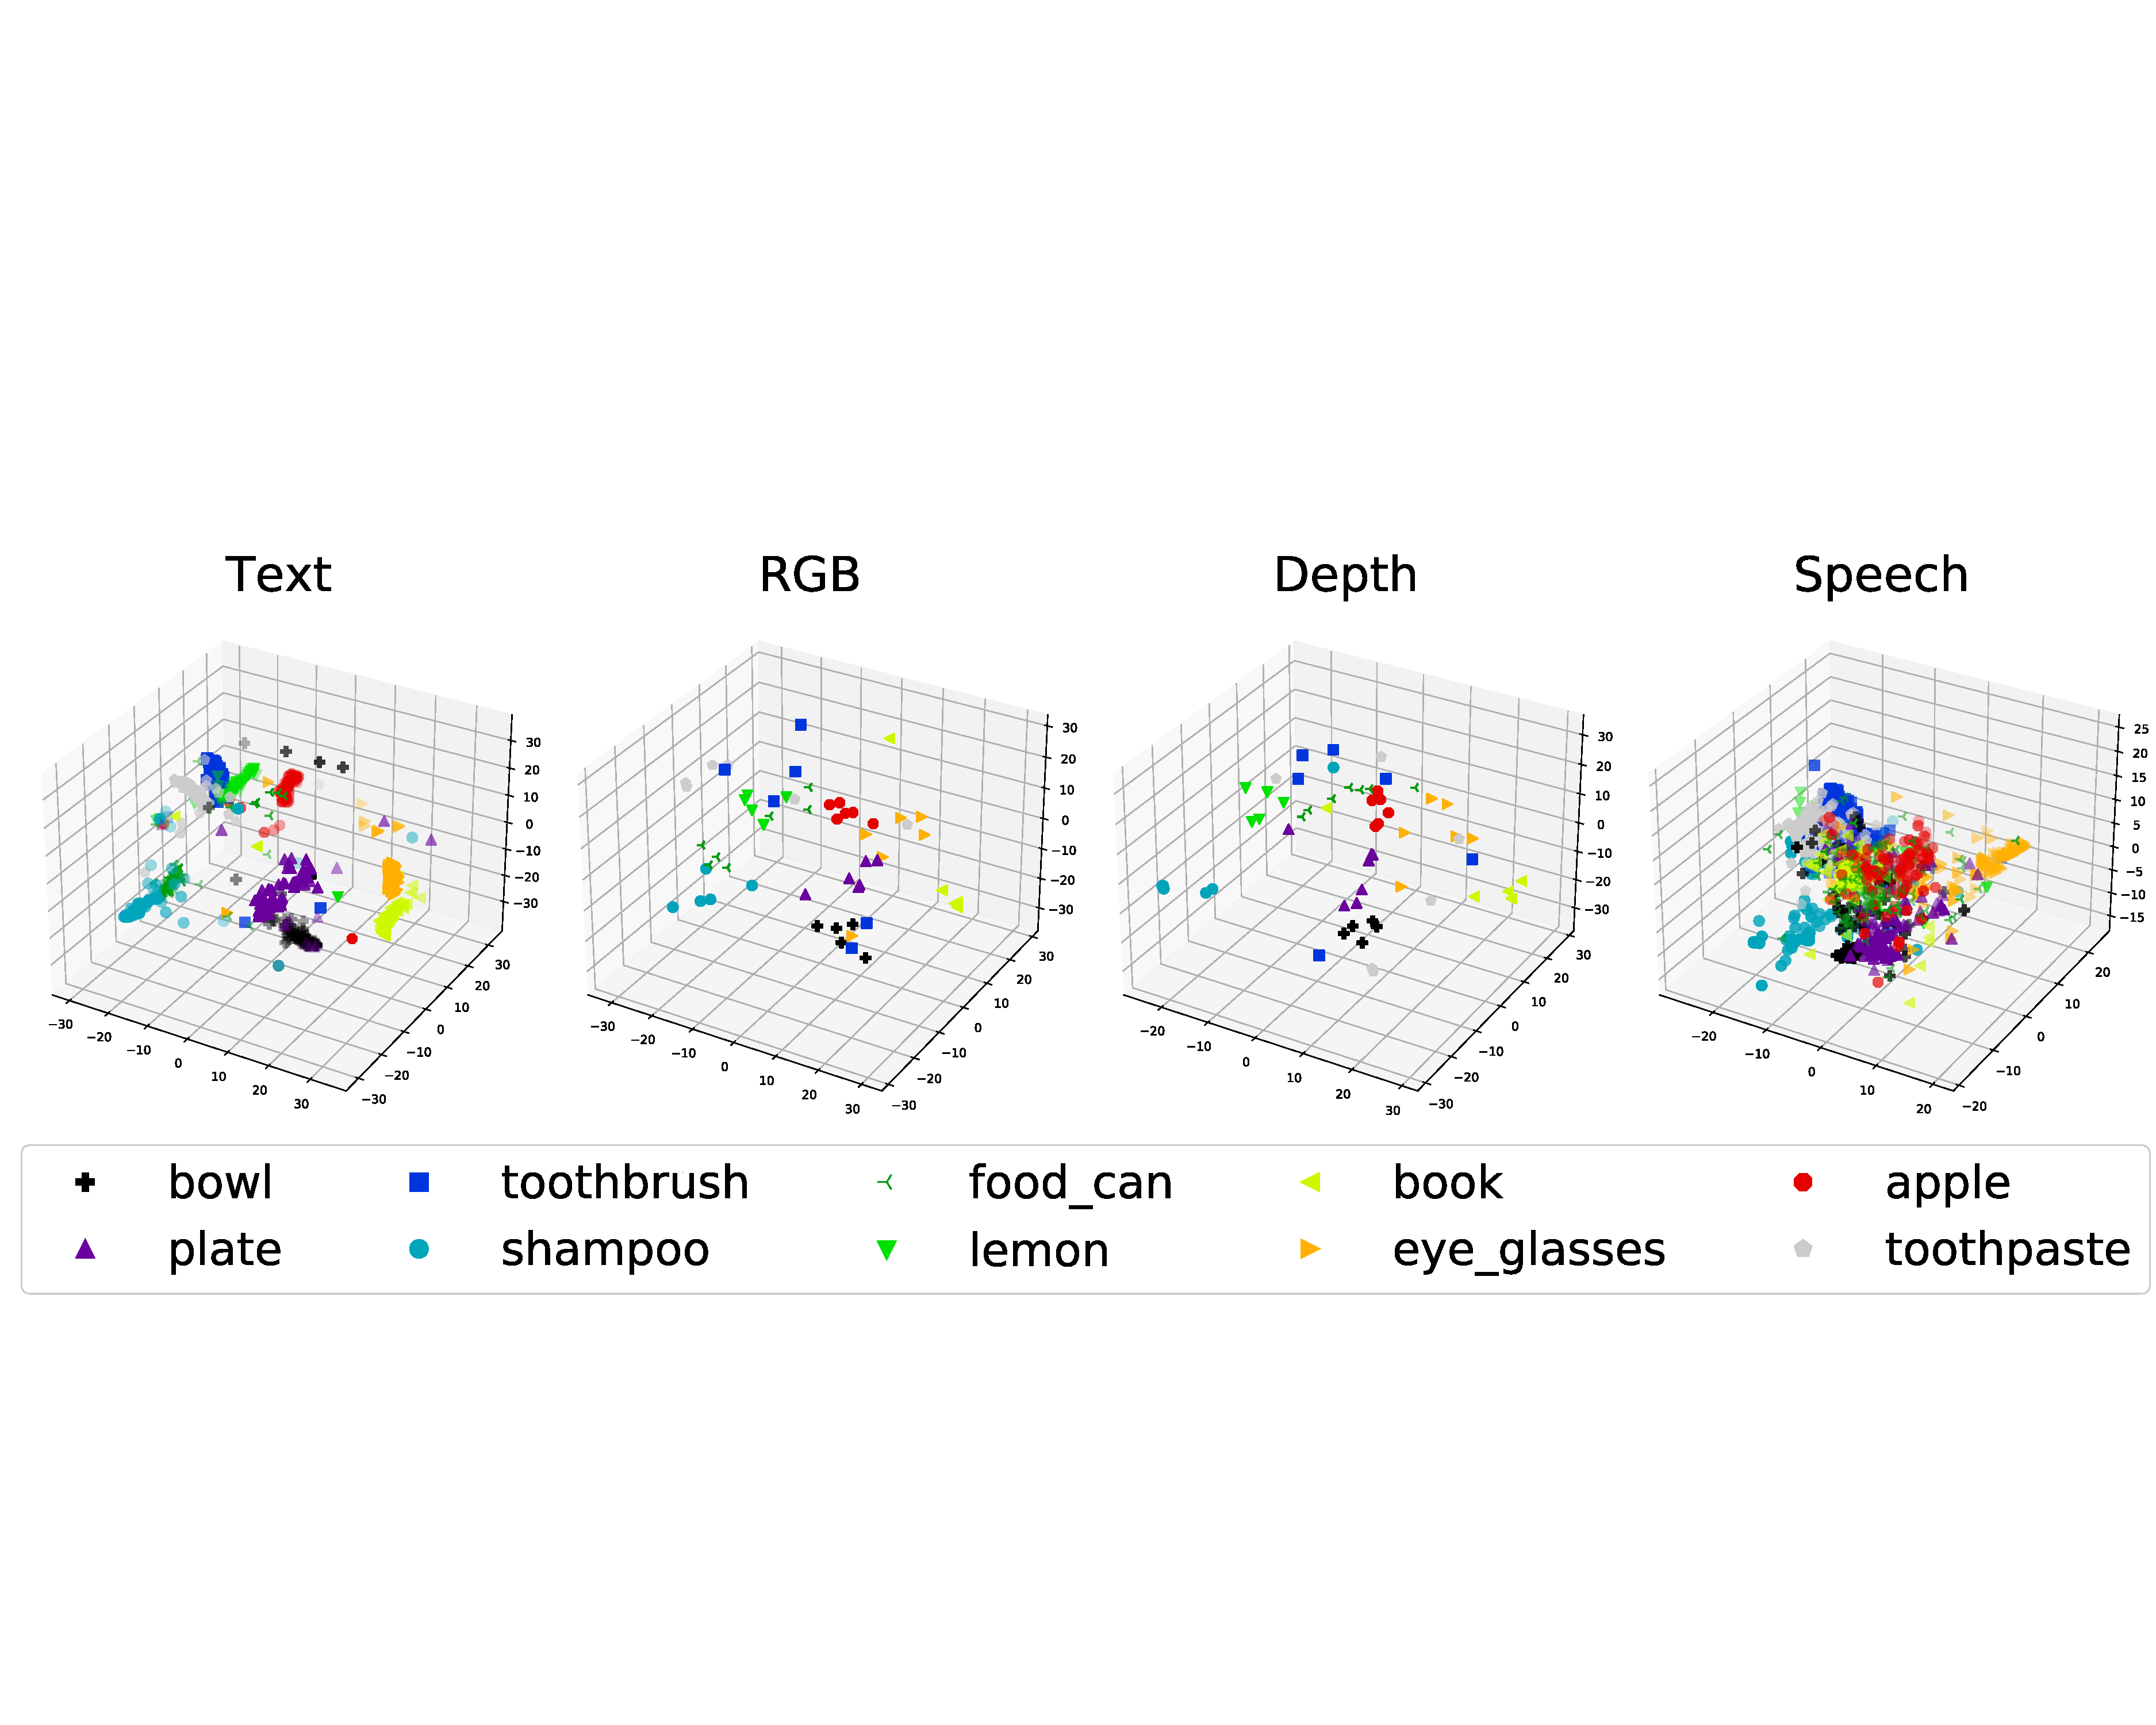
\includegraphics[width=.99\columnwidth]{Figures/3D-tsne-exp-supcon-emma-lard-64-relu-SGD-0.001-unique_objects-gold-no_neg_sampling-1024-trimmed.pdf}
\caption{3D T-SNE~\citep{van2008tsne} projection of test embeddings of 10 randomly selected classes of objects using \ours{}. Each modality is separately projected into a three-dimensional space. Each RGB and depth image is associated with several language descriptions, leading to denser plots for text and speech. In a perfect embedding, all instances of a class would be clustered in identical areas of the embedding space across all modalities. We can see that \ours{} successfully encourages all four modalities to live in a common manifold, allowing accurate retrieval even when modalities are missing.
}
% \todo[inline]{get rid of markers for modalities, and change the colors to be brighter. Try combining marker and color for each class.}

\label{fig:3d-tsne}
\end{figure*}

An example of the need to consider multiple modalities jointly is shown in \cref{fig:rankings}, showing how EMMA is able to correctly select an object instance from several similarly shaped and describable objects. 

\begin{figure}[h!]
\centering
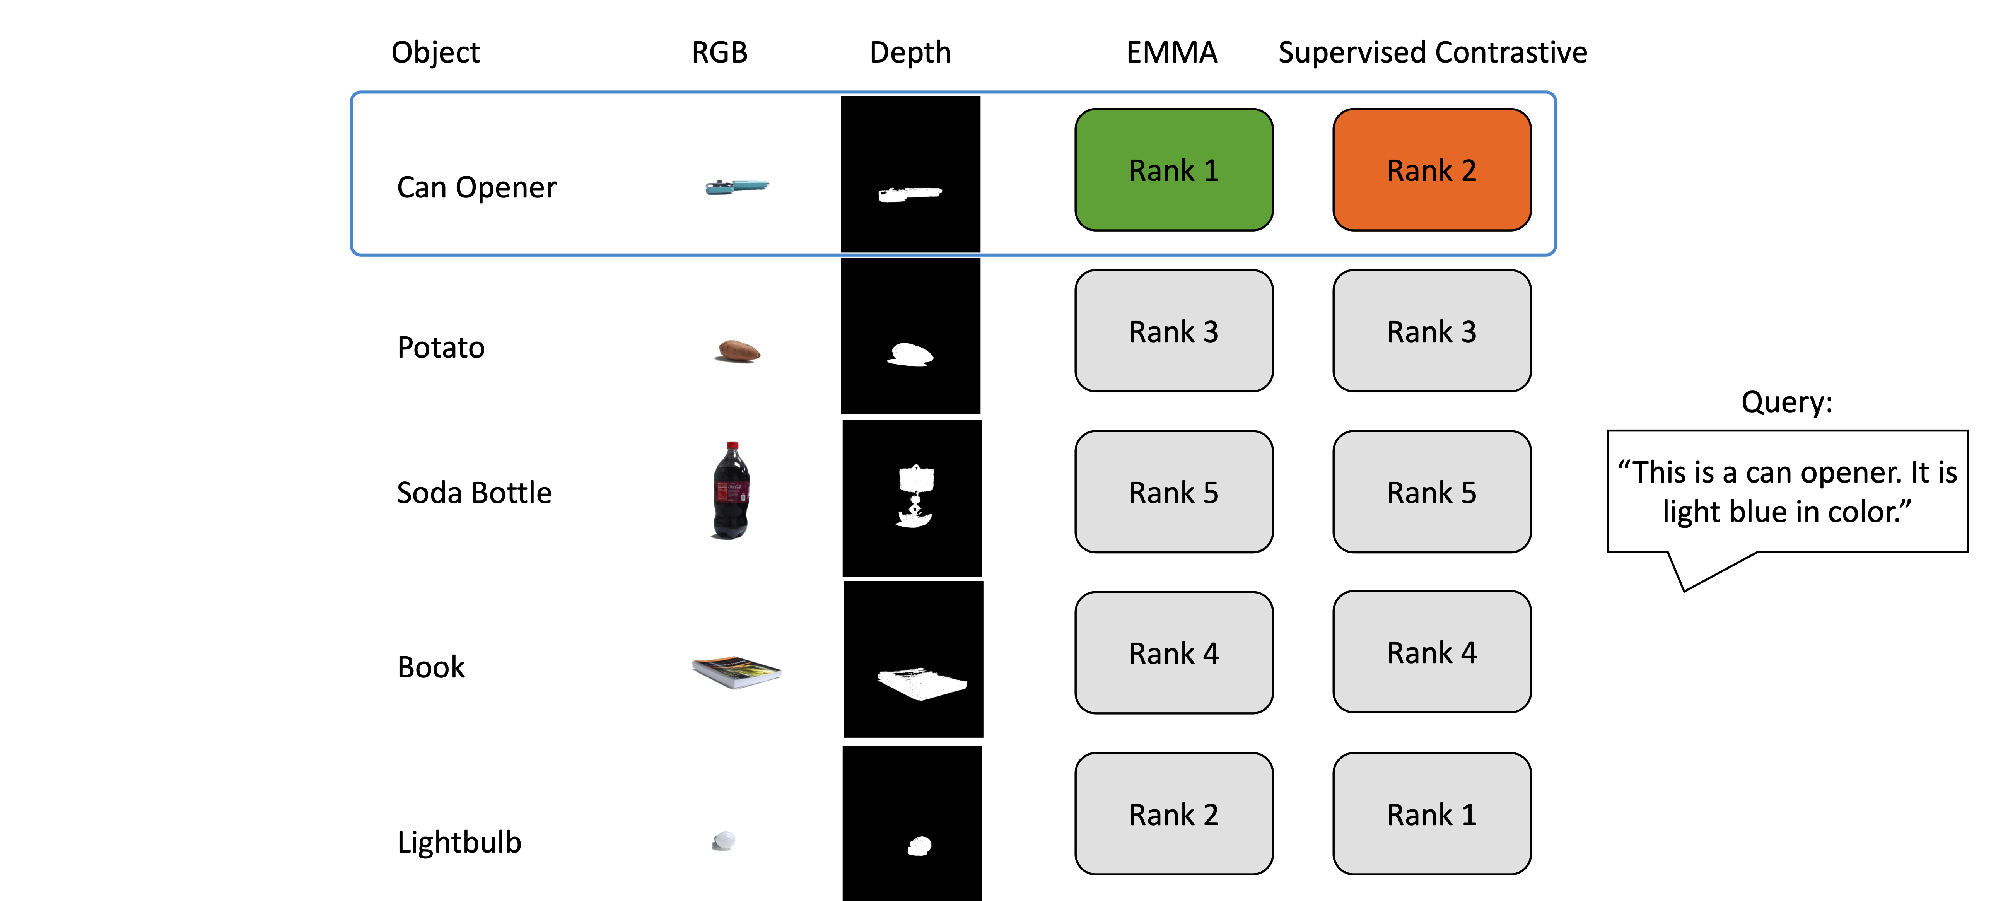
\includegraphics[width=.99\columnwidth]{Figures/example-rankings-rearranged}
\caption{\ours{} more accurately ranks objects and handles ambiguities with respect to a retrieval queries. Note that the phrase ``light blue'' in the query is very similar to ``light bulb'' and while \supcon{} confuses this and predicts light bulb as the correct object, \ours{} correctly identifies the can opener as the intended object, ranking the light bulb second.}
\label{fig:rankings}
\end{figure}


% \begin{figure}[tbh]
% \centering
% 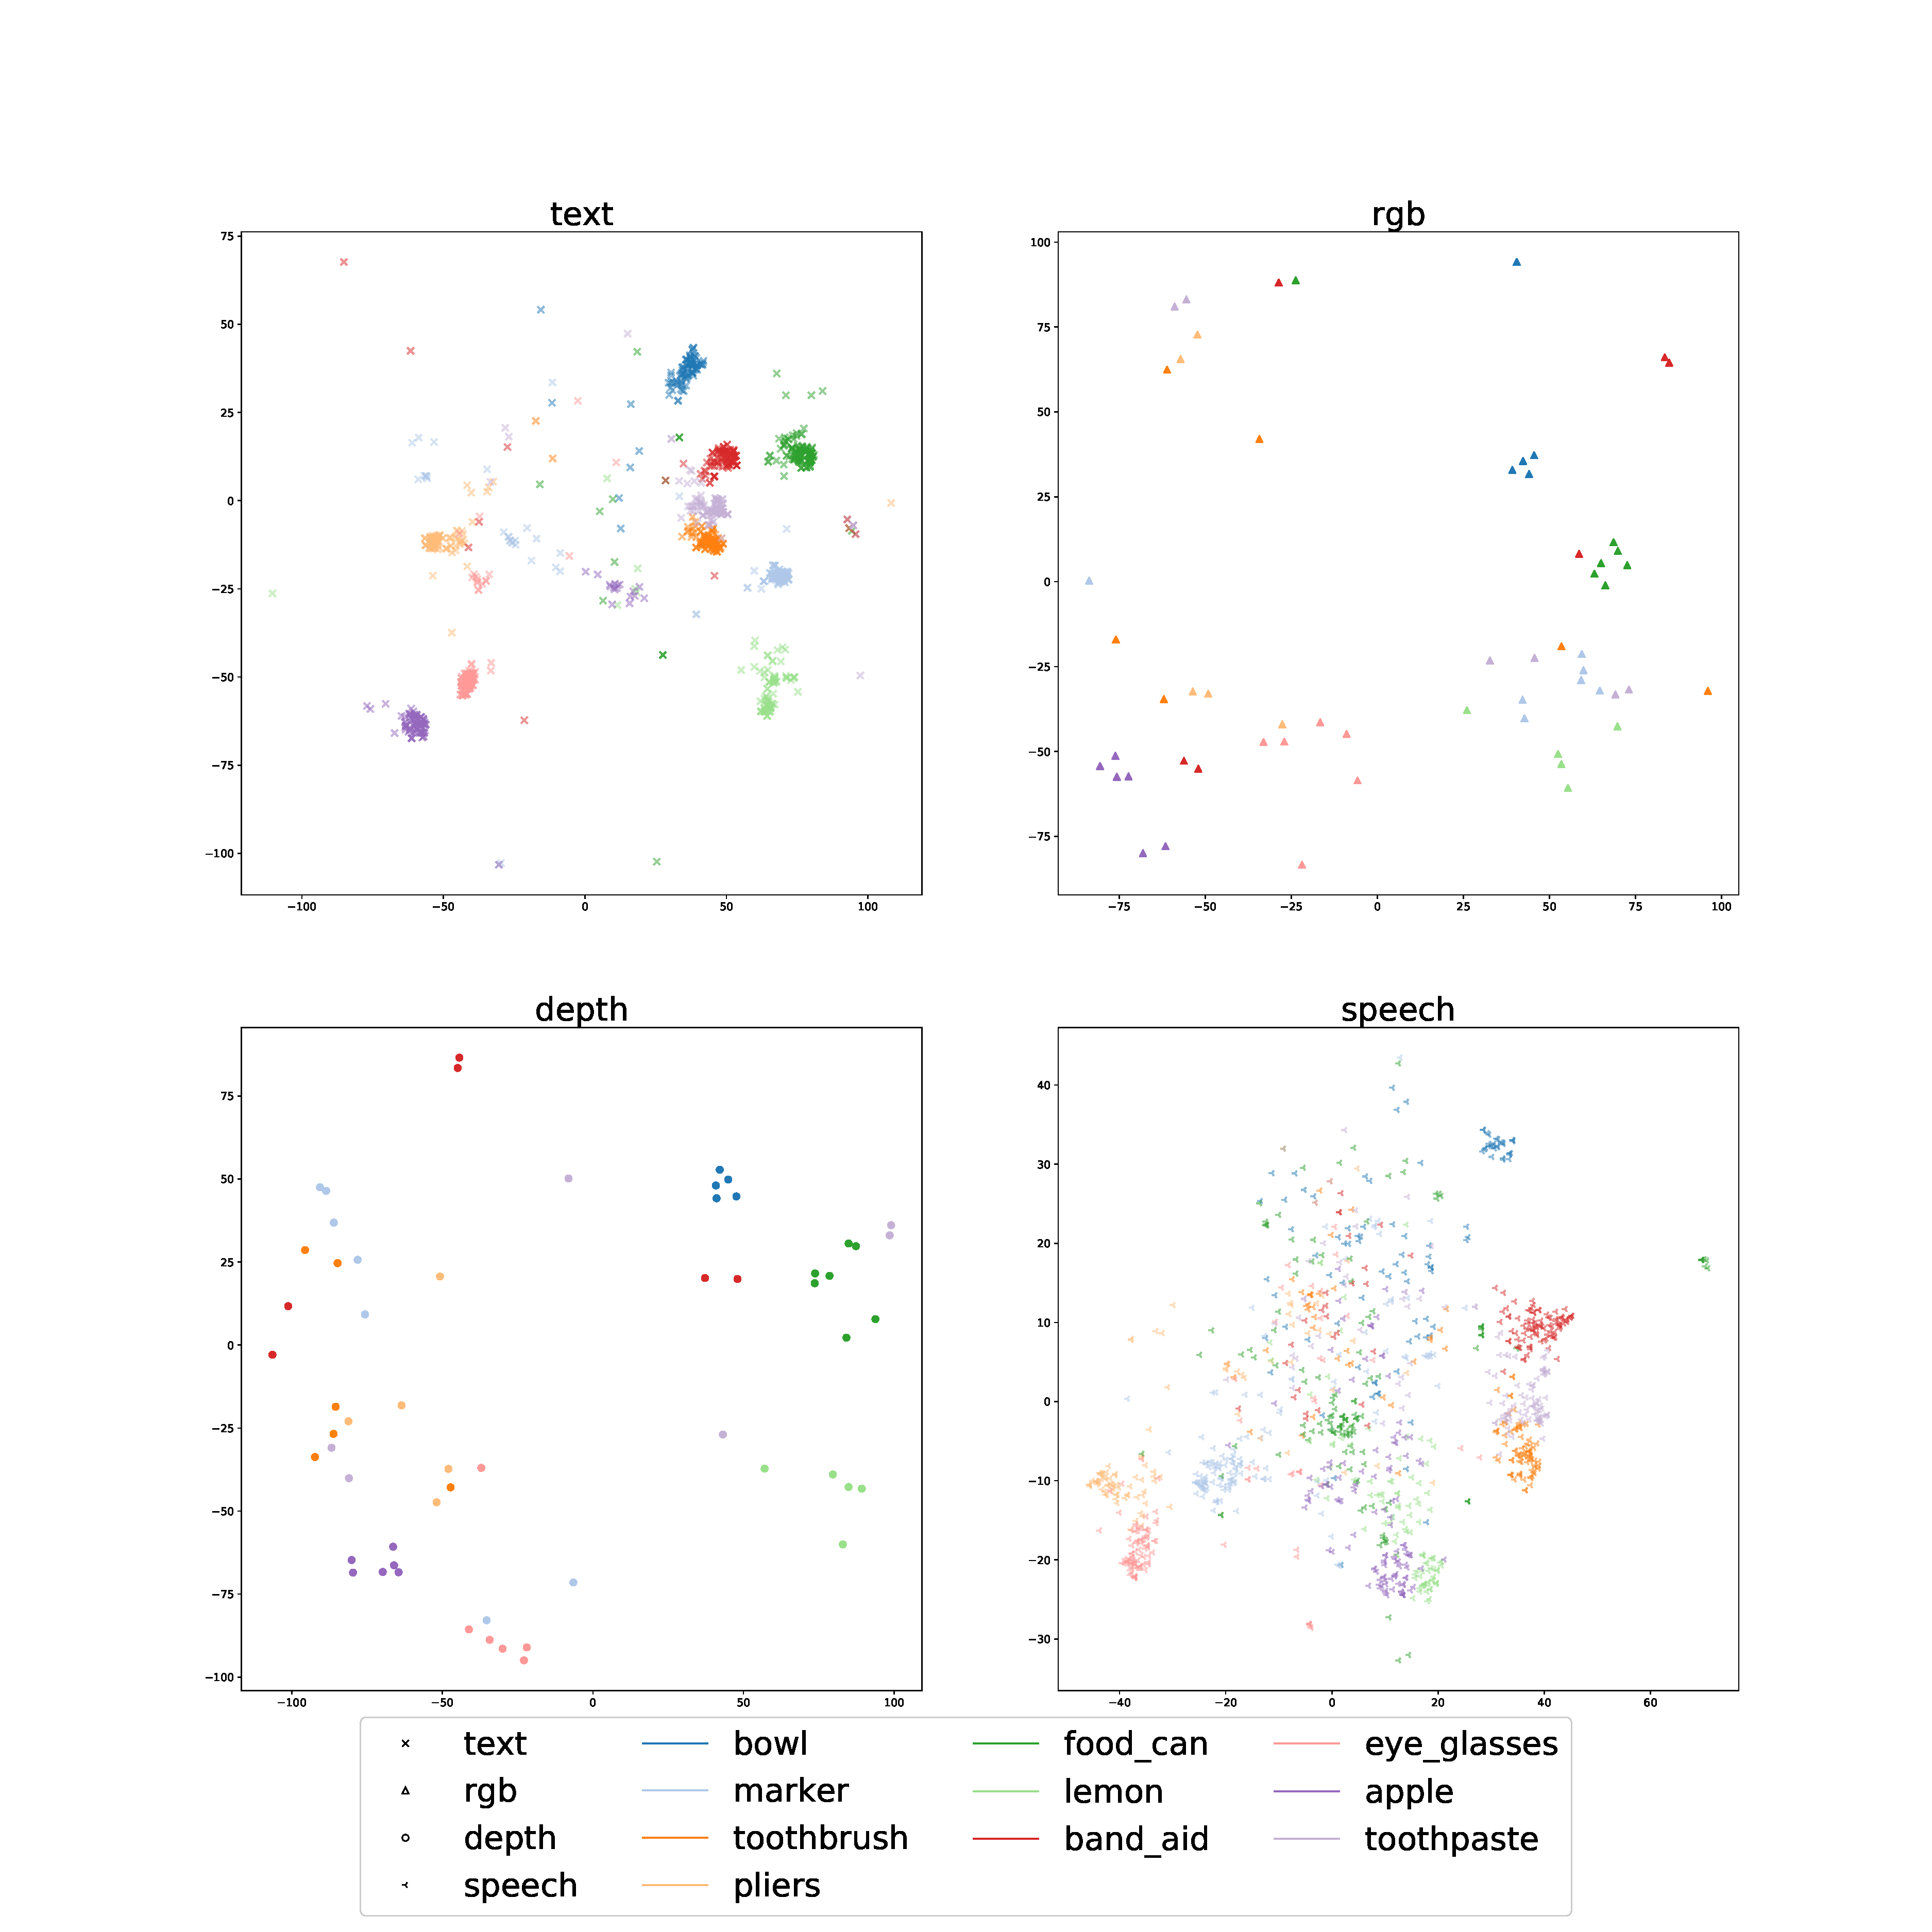
\includegraphics[width=.99\columnwidth]{Figures/2D-tsne-4M-eMMA-cosine-submodalities-text-anchor-gold-no_neg_sampling-1024.pdf}
% \caption{2D T-SNE~\citep{van2008tsne} projection of test embeddings of 10 randomly selected classes of objects using our proposed method. Each modality is separately projected into a two-dimensional space. \Rephrase{} \textcolor{red}{We may only want 3D}
% }
% \label{fig:2d-tsne}
% \end{figure}

% \todokdinline{Add the T-SNE projection for supervised contrastive loss as well.}

% \subsection{Failed Experiments}
% \todokdinline{I suppose I should remove this subsection, right?}
% We tried a lot of different approaches and they did not work better than our model or the baselines, but we list them here to save time for readers who want to try them.

% \subsubsection{Simple MMA}
% Copy text from \ref{sub:simple-mma} if we decide to keep this section.

% \subsubsection{Two Anchors}
% Since speech is similar to text in its usage when it comes to the downstream task of object retrieval (given a single language command, find the correct object among multiple objects), we decided to have text and speech as two anchors instead of having one anchor only. When there is one anchor, the distance between positive pairs text and speech is minimized and the distance between negative pairs are minimized. However, this is not related to the downstream task since we never want to find the correct speech for a given text or vice versa. The second term added to the last function is exactly similar to the loss function when speech is the anchor, and the first term is the same as when language is the anchor. Therefore, the performance is somewhere in the middle of those two approaches but more towards the speech when the metrics are computed based and speech matrices.

% \subsection{Example Prediction}



\subsection{Discussion}
Our proposed model performs well and learns fast, has been demonstrated to handle four modalities of shared information effectively, and is robust to test-time situations where information from one or more modalities is missing. There remains room for improvement. Specifically, the speech modality is harder to handle. \Cref{fig:3d-tsne} shows that although the relative position of instances are correct in the speech space, the distinction and clustering of different objects are not as good as the other three modalities.

Text seems to be the best clustered modality, and that makes sense because the variation in written text is much smaller than the other three modalities. Variation in speech is higher because there are a number of factors affecting speech understanding, including different accents, native language, gender, and age~\citep{KebeAAAI2022}. Variation in RGB and depth is higher than in text due to variations in lighting conditions, an object's texture and shape, the angle of the camera, and other factors.


%===================================================================

\section{Conclusion}
\label{sec:conclusion}


In this work, we have demonstrated the effectiveness of a novel approach to learning from high-dimensional multimodal information even when one or more modalities is unavailable at test time. Our approach performs well on an object retrieval task from a testbed that contains four separate modalities, consistent with information that might be available to a physical agent, and outperforms state of the art contrastive learning approaches. 
Our proposed method is general enough to be applied to a variety of multimodal retrieval problems, and is not limited to purely language-based image retrieval.
% \todokdinline{Don't we need evidence for that?}

In future, this work will be extended to solve less clearly delineated problems; for example, differentiating among members of a class, as well as across classes. However, this work represents a significant step towards handling such retrieval problems, while not arbitrarily limiting the number of sensor and other modalities that can be incorporated. 

% Another future work is to improve the speech modality so it can contribute more to the training. Right now when text modality is dropped, the performance decreases by about 0.12. Ideally a better model should have the same performance in case of dropout when it is trained using all modalities.

%===================================================================


% ***************** The END of the paper *****************



\bibliography{tmlr}
\bibliographystyle{tmlr}

\appendix
\label{sec:appendix}
% \todocmi{should we get rid of this appendix? I am thinking so.}
% 
\section{Qualitative Analysis}
\section{Approach}

For $M$ modalities, we define a distance based loss function which is a generalization of well-known similarity-based metric learning and manifold alignment methods such as triplet loss~\cite{Carvalho-cooking-triplet,triplet_loss_2021_CVPR}, quadruplet loss~\cite{chen2017beyond}, and is similar to contrastive loss under some settings.
We sample two data points from each modality, one positive point and one negative point. 
For each set of positive data points (referring to an instance of an object with all of its modalities), we choose a set of negative data points either based on object class name, or by semantic negative sampling~\cite{Pillai_Matuszek_2018}. We now have two data points; we consider the first one as positive, and the second one as negative. However, the anchor won't be another data point as it is in the triplet loss terminology. Instead we choose one domain as an anchor. 

\begin{itemize}
    % \item data point: a row in the csv/tsv file.
    \item Positive: a set of embeddings of the one data point (RGB image of an apple, corresponding depth image, text description, and speech description of the same apple)
    \item Negative: a set of embeddings of the another data point of a different object (RGB image of a book, corresponding depth image, text description, and speech description of the same book)
    \item Anchor: A fixed modality to act as anchor in the case of simple MMA loss, where we don't minimize the distance between the pair of embeddings from all modalities of the same data point, and we don't maximize the distance between positive an negative datapoints of the same modality.
\end{itemize}

The objective is then to (I) minimize the distance between each pair of positive points from heterogeneous modalities which results in $(M-1)!$ terms, (II) maximize the distance between each pair of positive and negative points from heterogeneous modalities which contains $(M-1)!$ terms again, and (III) maximize the distance between each pair of positive and negative points from the homogeneous modalities which contains $M$ terms. Altogether, our proposed loss function contains $M+2(M-1)!$ terms.
\Cref{eq:objective} shows the objective function we defined above with changing maximization to minimization by changing the sign.

% \begin{equation}\label{eq:objective-detailed}
%     \min \sum_{i=1}^{M-1} \sum_{j=i+1}^{M} ||x_{i}^{+} - x_{j}^{+}|| - \sum_{i=1}^{M-1} \sum_{j=i+1}^{N} ||x_{i}^{+} - x_{j}^{-}|| - 
%     \sum_{i=1}^{M} ||x_{i}^{+} - x_{i}^{-}||
% \end{equation}


% \begin{equation}\label{eq:objective}
% \begin{split}
%     \mathcal{L}  &= \sum_{i=1}^{M-1} \sum_{j=i+1}^{M} ||f_i(x_{i}^{+}) - f_j(x_{j}^{+})|| \\
%     & - ||f_i(x_{i}^{+}) - f_j(x_{j}^{-})||
%     - ||f_i(x_{i}^{-}) - f_j(x_{j}^{+})|| \\
%     & - \sum_{i=1}^{M} ||f_i(x_{i}^{+}) - f_i(x_{i}^{-}) ||
% \end{split}
% \end{equation}
% where $f_i(.)$ and $f_j(.)$ represent functions that map input data to the shared latent space using a deep neural network.


% d(,) notation instead of || - ||
% \begin{equation}\label{eq:objective}
% \begin{split}
%     \mathcal{L}  &= \sum_{i=1}^{M-1} \sum_{j=i+1}^{M} d(z_{i}^{+}, z_{j}^{+}) 
%      - d(z_{i}^{+}, z_{j}^{-}) \\ 
%     & - d(z_{i}^{-}, z_{j}^{+}) - \sum_{i=1}^{M} d(z_{i}^{+}, z_{i}^{-})
% \end{split}
% \end{equation}

\begin{equation}\label{eq:objective}
\begin{split}
    \mathcal{L}  &= \sum_{i=1}^{M-1} \sum_{j=i+1}^{M} ||z_{i}^{+} - z_{j}^{+}|| 
     - ||z_{i}^{+} - z_{j}^{-}|| - ||z_{i}^{-} - z_{j}^{+}|| \\ 
    &  - \sum_{i=1}^{M} ||z_{i}^{+} - z_{i}^{-} ||
\end{split}
\end{equation}
where the subscripts $i$ and $j$ represent modalities, and $z$ is the embedding we get by applying a mapping function $f$ which in our case is a neural network on our input data. In other words $z_m = f_m(x_m)$ where each modality $m$ has a specific model $f_m$ that is different from the models for other modalities and these models do not share their weights. 
To measure the distance, we use cosine distance.
In order to use cosine \textit{distance}, we have to subtract the cosine of the \textit{angle} between two embeddings (which represents similarity) from 1: $1 - \cos(e_1, e_2)$.

\todokdinline{I can add another term for minimizing the distance between similar pairs (anchor and positive) from the same domain. This would look like the equation below. However, it breaks the nice procedure of sampling two data points per modality}
\todo{Edward wonders if $f_i(x)$ should instead produce $\mu_x$ and $\Sigma_x$, to capture uncertainty of embedding location, when working with so many modalities? (e.g., not all modalities share the same ambiguities)}
\todo{Does Edward mean the actual network produces $\Sigma_x$, e.g., something like a VAE? How would uncertainty be applied to the inference problem?}
$+ \sum_{i=1}^{M} ||f_i(x_i^{a}) - f_i(x_i^{+})||$


If $M=2$ which means the number of modalities is 2, then our objective function reduces to the quadruplet loss method~\cite{chen2017beyond} if we ignore the third term, and negative samples for each modality do not belong to the same class.
If $M=2$ and we ignore the last two terms in the objective function, it results in the triplet loss method. 
If $M=1$, only the last term remains in the loss function which is exactly the pairwise distance-based loss function.


We demonstrate performance using three different distance-based loss functions.
\todokdinline{Either remove it or experiment with all versions of MMA (12 terms, 9 terms, and explicit anchor maximization}

\subsection{Simple MMA}
\label{sub:simple-mma}
Our first proposed loss function is a modification of the triplet loss function idea, and can be derived from \cref{eq:objective} by fixing one modality as anchor, and ignoring the last two terms in \cref{eq:objective}.

% For each data point (referring to an instance of an object with all of its modalities), we choose a negative data point either based on object class name, or by semantic negative sampling~\cite{Pillai_Matuszek_2018}. We now have two data points; we consider the first one as positive, and the second one as negative. However, the anchor won't be another data point as it is in the triplet loss terminology. Instead we choose one domain as an anchor. 

% \begin{itemize}
%     % \item data point: a row in the csv/tsv file.
%     \item Positive: a set of embeddings of the one data point (RGB image of an apple, depth image of an apple, language description of an apple)
%     \item Negative: a set of embeddings of the another data point of a different object (RGB image of a book, depth image of a book, language description of a book)
%     \item Anchor: A fixed modality to act as anchor in the case of simple MMA loss, where we don't minimize the distance between the pair of embeddings from all modalities of the same data point, and we don't maximize the distance between positive an negative datapoints of the same modality.
% \end{itemize}

Since the downstream task in the grounded language learning domain is to predict/retrieve a desired object among multiple objects given a natural language description, it makes sense to train the model using language as an anchor, and in fact anchoring learning around language outperforms anchoring on RGB.

\Cref{eq:objective-simple-mma} shows the mathematical formulation of the proposed loss function which can be generalized to arbitrary number of modalities.

% \begin{equation}
% \label{eq:objective-simple-mma}
% \begin{split}
%     \mathcal{L}  &= \sum_{m=1}^{M-1} || f_a(x_{a}^{+}) - f_m(x_{m}^{+}) || - \\ 
%     & || f_a(x_{a}^{+}) -f_m(x_{m}^{-}) || 
%     \\
%     &= \sum_{m=1}^{M-1} 1 - \cos(f_a(x_{a}^{+}), f_m(x_{m}^{+})) \\ & - (1 - \cos(f_a(x_{a}^{+}) ,f_m(x_{m}^{-}))) \\
%     &= \sum_{m=1}^{M-1} \cos(f_a(x_{a}^{+}) ,f_m(x_{m}^{-})) \\ 
%     & - \cos(f_a(x_{a}^{+}), f_m(x_{m}^{+}))
% \end{split}
% \end{equation}

\begin{equation}
\label{eq:objective-simple-mma}
\begin{split}
    \mathcal{L}  &= \sum_{m=1}^{M-1} || z_{a}^{+} - z_{m}^{+} || - || z_{a}^{+} - z_{m}^{-} || \\
    &= \sum_{m=1}^{M-1} 1 - \cos(z_{a}^{+}, z_{m}^{+}) - (1 - \cos(z_{a}^{+}, z_{m}^{-})) \\
    &= \sum_{m=1}^{M-1} \cos(z_{a}^{+} ,z_{m}^{-}) - \cos(z_{a}^{+}, z_{m}^{+})
\end{split}
\end{equation}

where subscript $a$ represents \textit{anchor} modality, $M$ is the number of modalities, superscript $+$ represents the positive objects, and superscript $-$ represents the negative objects.

An illustration of this loss function is provided in \cref{fig:simple-mma-loss}.

\begin{figure}[tb]
\centering
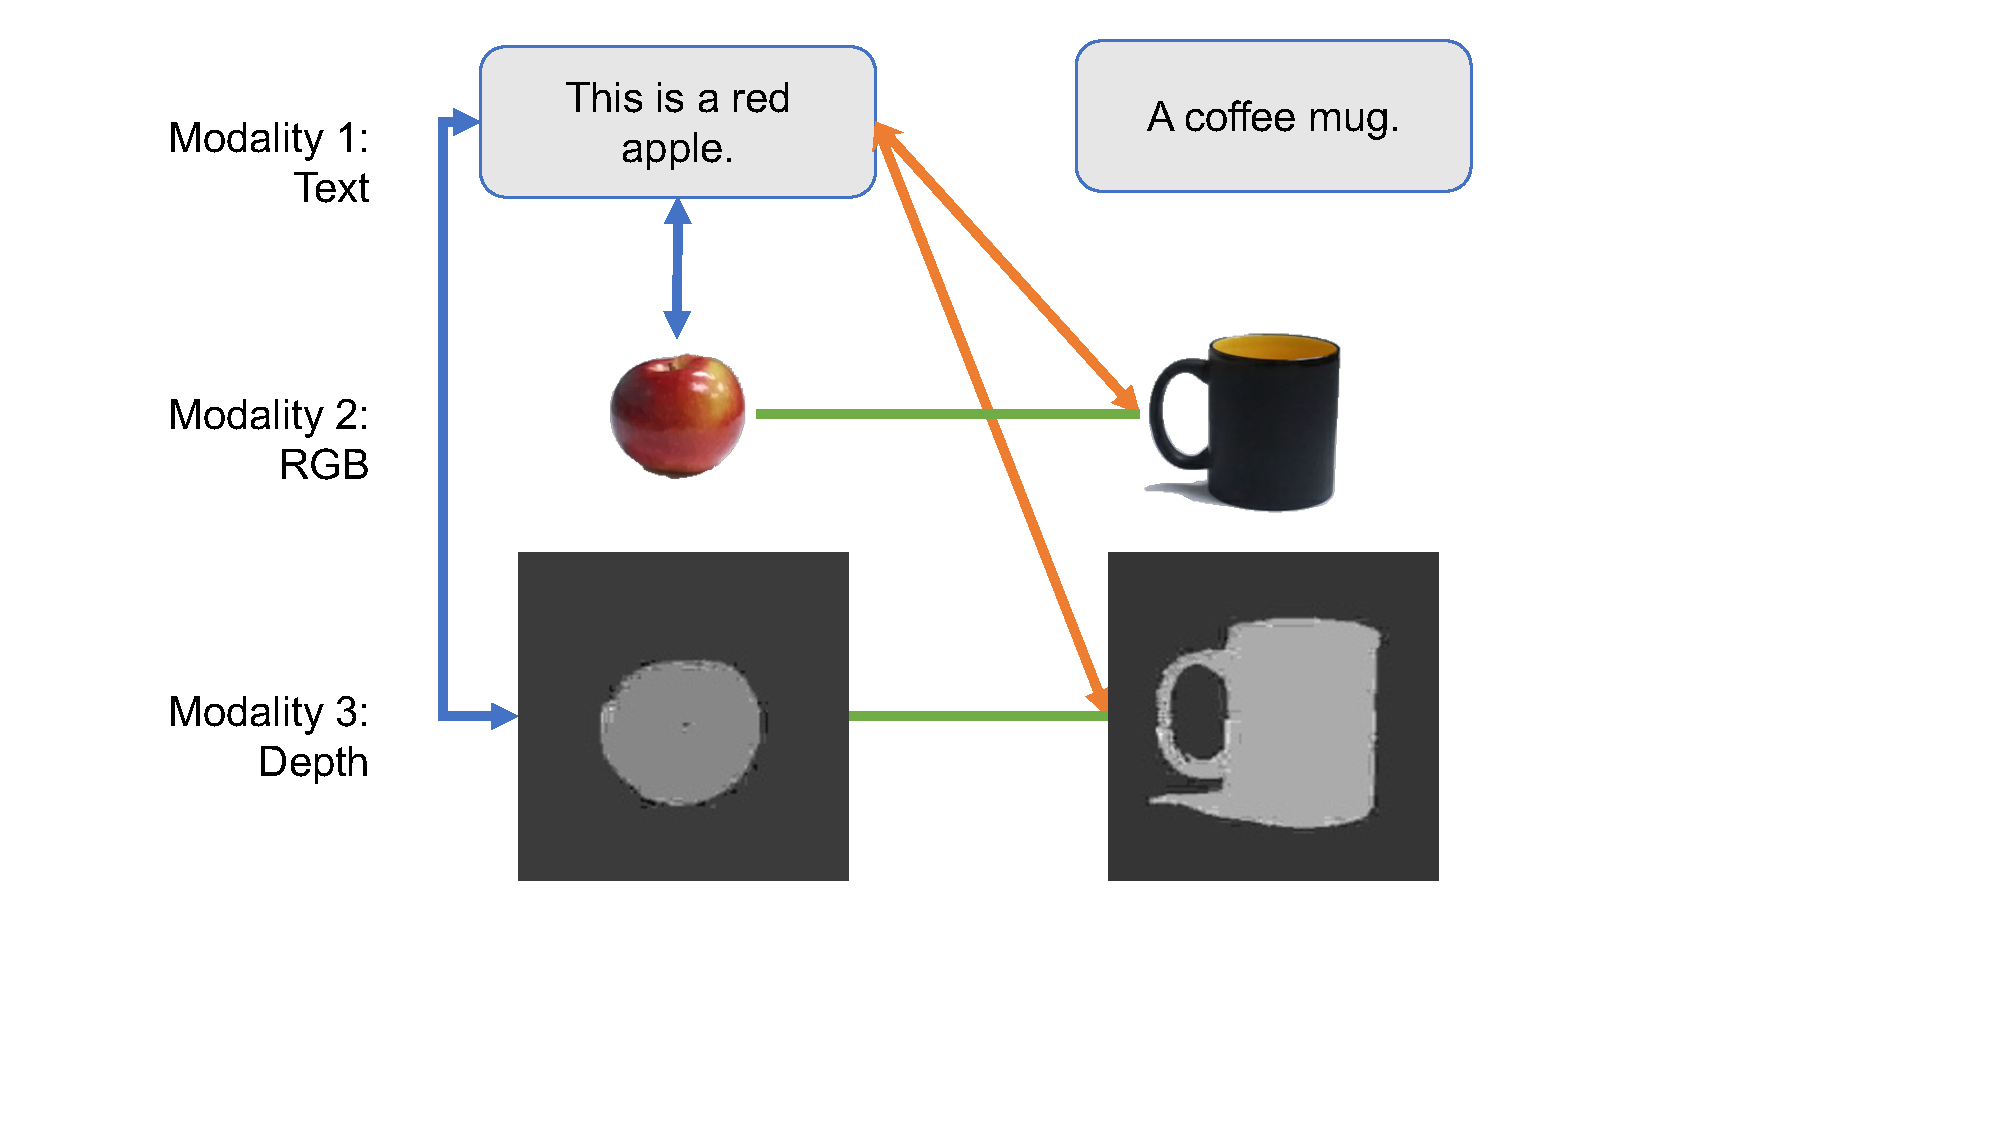
\includegraphics[width=\columnwidth]{Figures/simple-MMA.pdf}
\caption{A high-level prototype of the distances used in the simple MMA loss with 3 modalities. Orange arrows indicate maximizing the distance, blue arrows indicate minimizing the distance, and green lines show the margin. Depth images are brightened to be visible. \todo[inline]{We need to show speech as the 4th modality as well.}}
\label{fig:simple-mma-loss}
\end{figure}

This version of MMA loss function can be seen as a contrastive loss usually used in the domain of self-supervised learning~\cite{chen2020simple}. However, our proposed loss function has two advantages over the traditional contrastive loss expressed in \cref{eq:contrastive-loss}. The first advantage is that our loss function do not loop over multiple positives and negatives in a large batch. Instead we sample only two objects (positive and negative) each of which have $M$ modalities which gives us $2M$ datapoints (or embeddings). Hence, our model can be trained using smaller batch sizes and reduces the number of negative samples we need. The second advantage is that this loss function can be used in a multimodal setting with an arbitrary number of modalities, and is not limited to a single data type (e.g. RGB images) which is the most common usage of contrastive loss~\cite{chen2020simple, NEURIPS2020_supervised_contrastive}.


Therefore, our proposed loss function would modify \cref{eq:contrastive-loss} to the loss function formulated in \cref{eq:simple-MMA-contrastive}. Our formulation is a generalized version of the contrastive loss where $M$ is the number of modalities (e.g. RGB image, depth image, speech, text), but it can be the ``augmented views'' instead of different modalities.

% \begin{equation}\label{eq:simple-MMA-contrastive}
%     -\sum_{m=1}^{M-1} \log \frac{\exp (sim(f_a(x_a^+) , f_m(x_{m}^{+})/ \tau) )}{ \exp (sim(f_a(x_a^+) , f_m(x_{m}^{+}) / \tau)) + \exp (sim(f_a(x_a^+), f_m(x_{m}^{-}) / \tau))}
% \end{equation}

\begin{equation}\label{eq:simple-MMA-contrastive}
    -\sum_{m=1}^{M-1} \log \frac{\exp (sim(z_a^+ , z_{m}^{+})/ \tau) }{ \exp (sim(z_a^+ , z_{m}^{+}) / \tau) + \exp (sim(z_a^+, z_{m}^{-}) / \tau)}
\end{equation}
where $z = f(x)$.

% \todokdinline{I should run the traditional contrastive loss to see if my method works better to make this claim.}



% \subsubsection{All in loss with 12 terms}
% \subsubsection{subset of All in loss with 9 terms}

\section{Data}

\begin{figure*}[tbh]
\centering
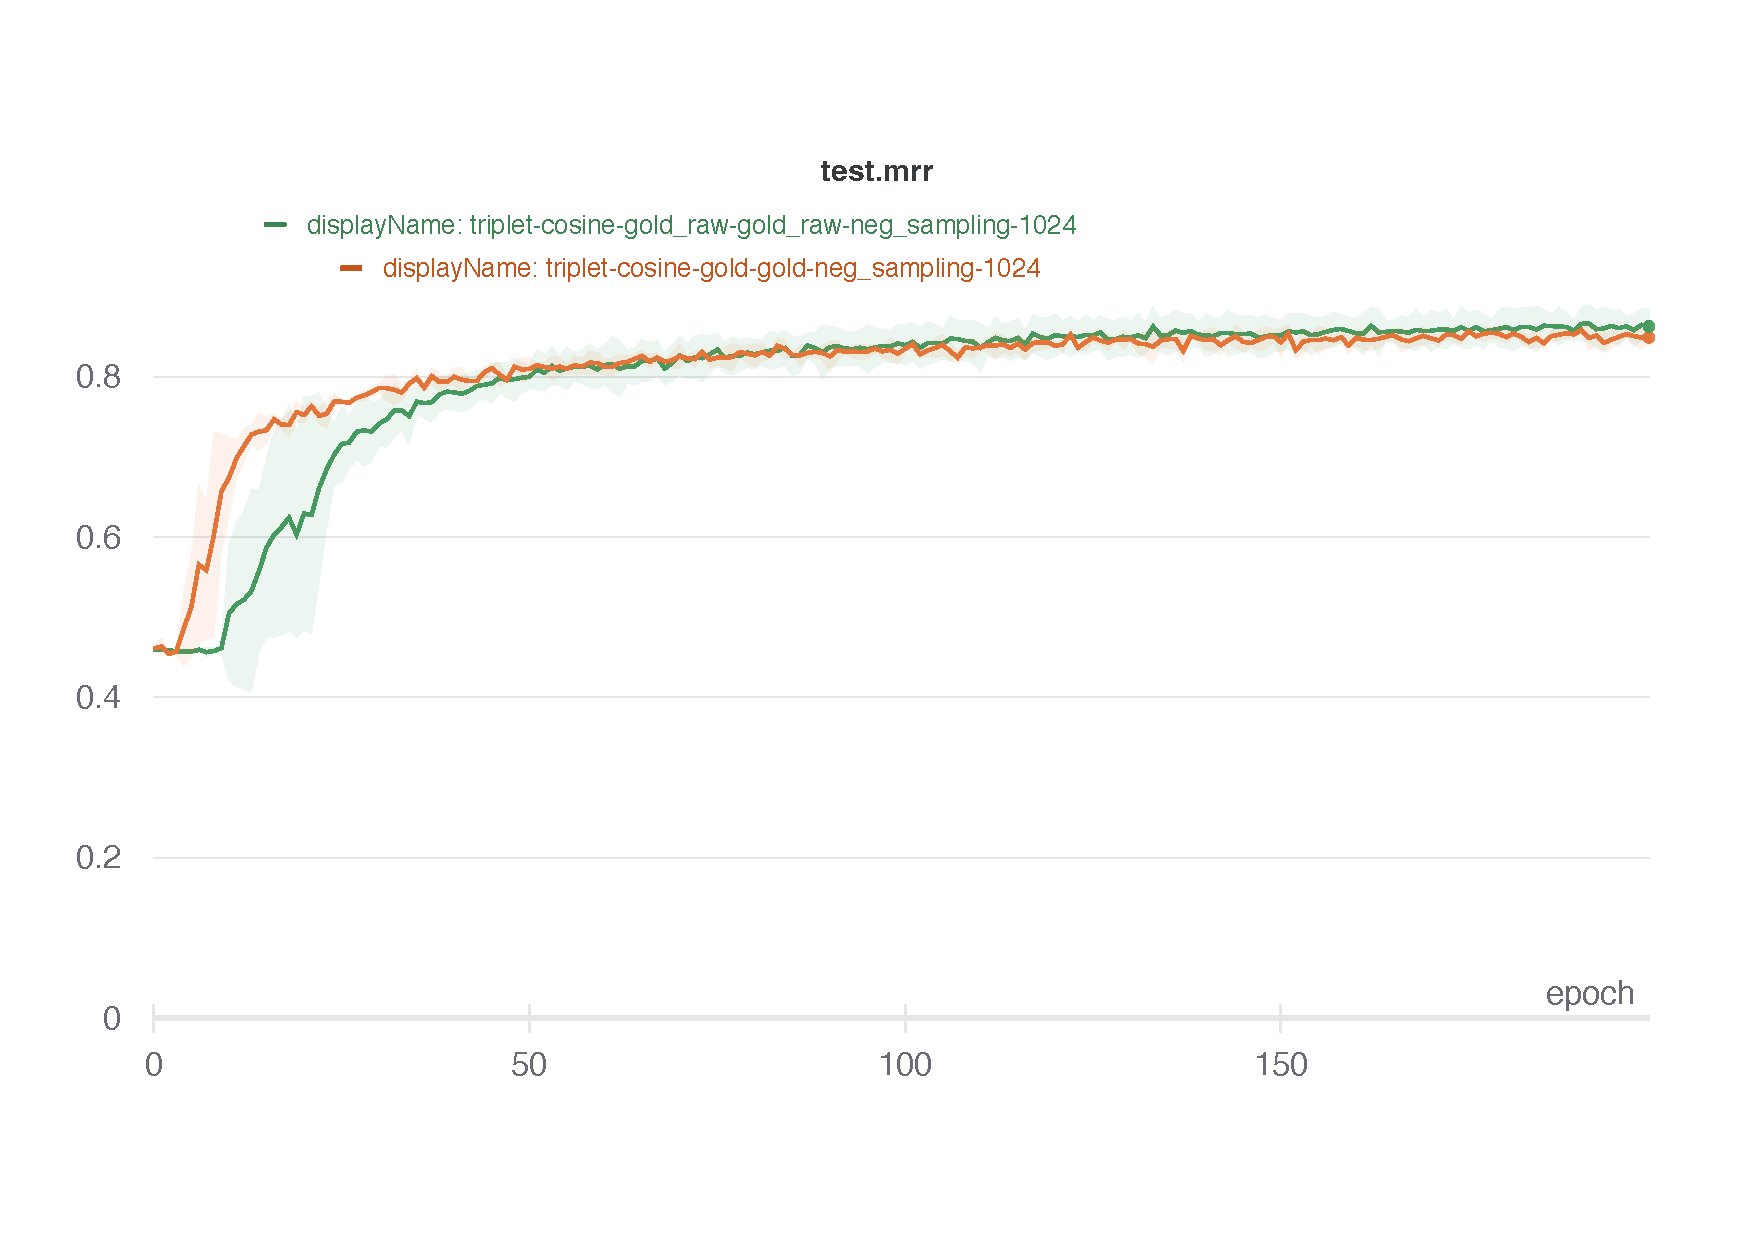
\includegraphics[width=2.0\columnwidth]{Figures/raw-mask-test-mrr.pdf}
\caption{Mean Reciprocal Rank (MRR) on different versions of GoLD dataset~\cite{GoLD_UMBC}. The raw version is depicted in green and masked version is depicted in orange averaged over 3 different random seeds. Higher is better.}
\label{fig:mask-vs-raw}
\end{figure*}

\section{Experiments}

\section{Results}

\begin{figure*}[tbh]
\centering
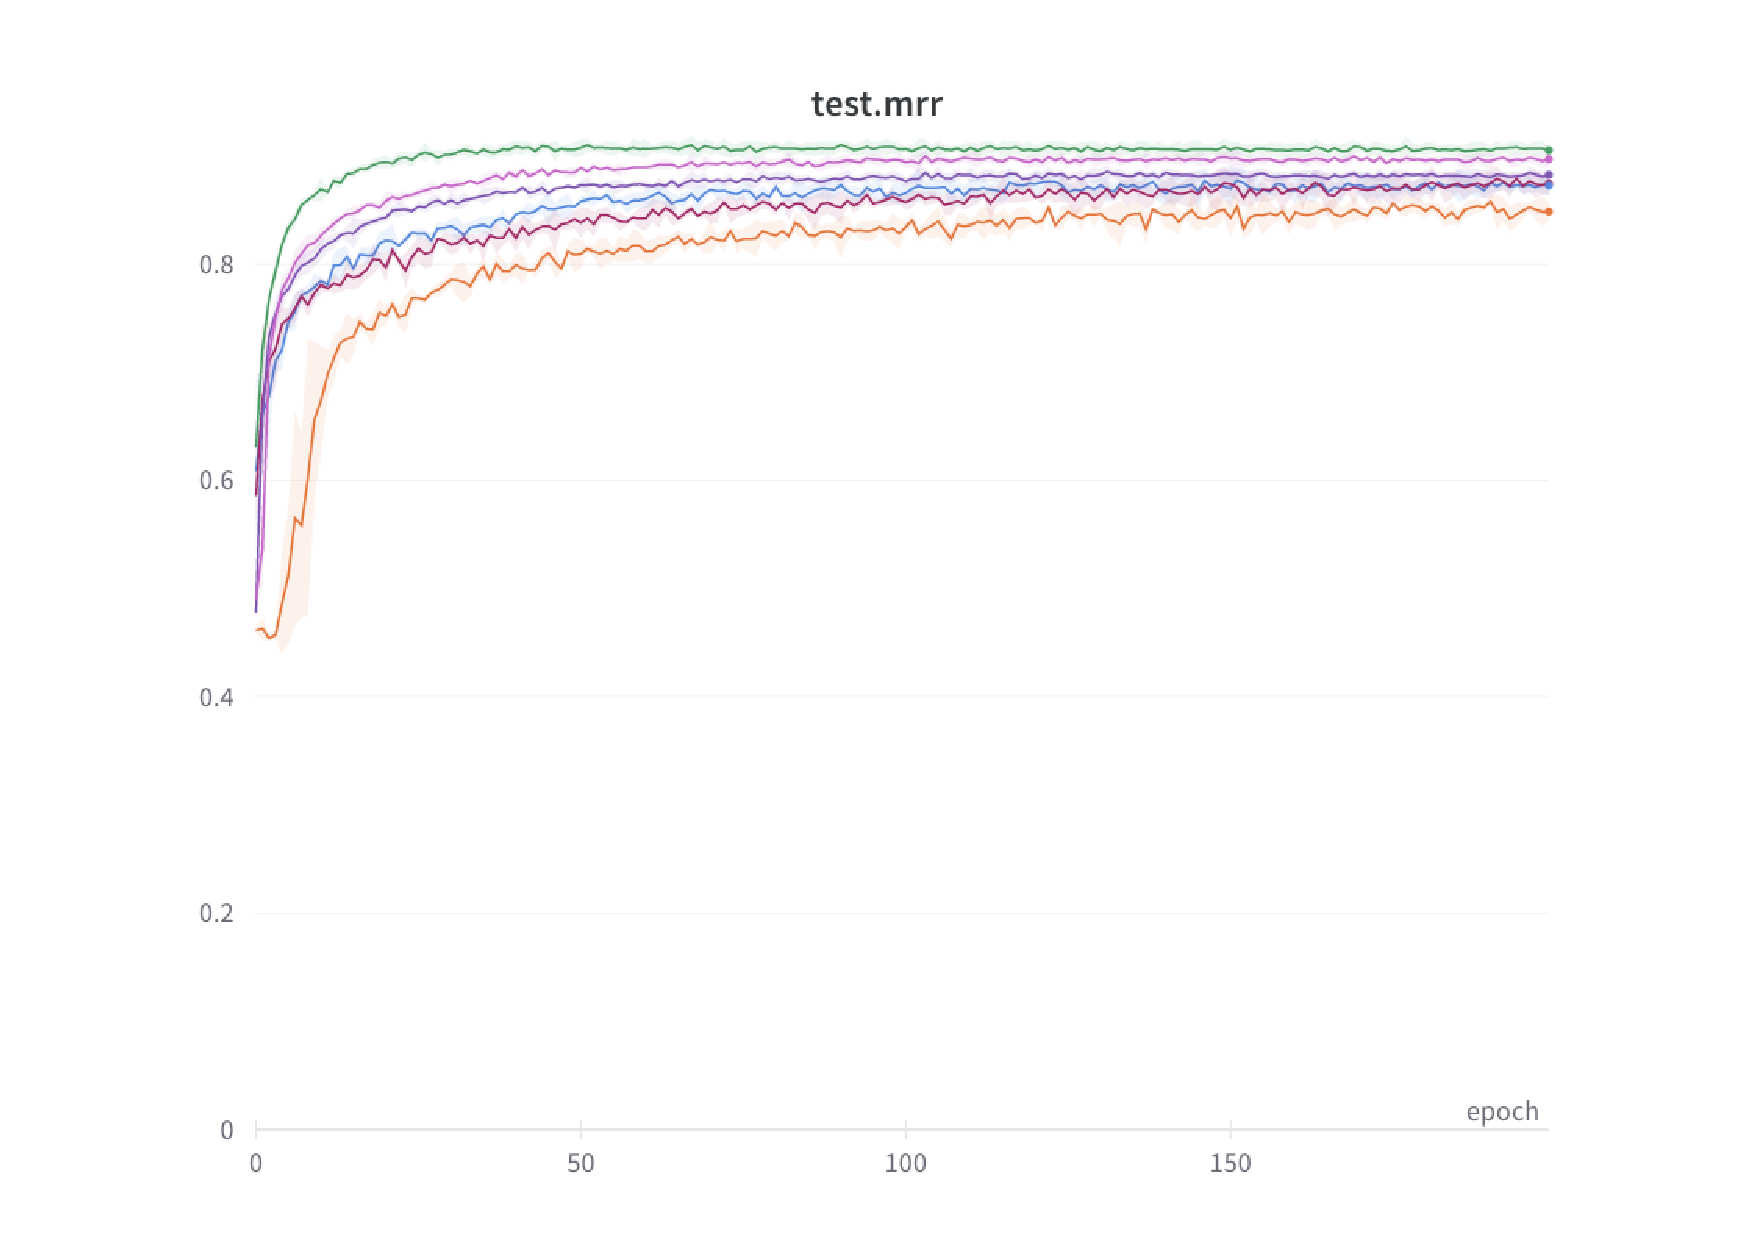
\includegraphics[width=2.1\columnwidth]{Figures/test.mrr.pdf}
\caption{Mean Reciprocal Rank (MRR) of our proposed method against triplet loss method averaged over 3 different random seeds for a downstream task of object detection. The higher is better. Green is Supervised Contrastive Learning~\cite{NEURIPS2020_supervised_contrastive}, Pink represents our proposed simple MMA loss function without semantic negative sampling w/ SGD w/ adjusting learning rate, Purple is out method with semantic negative sampling, Blue is our method w/ semantic negative sampling w/ Adam and w/o adjusting learning rate, Red is vanilla contrastive loss with cosine, and orange represent the triplet loss. function~\cite{triplet_loss_2021_CVPR}.
}

\label{fig:simple-MMA-mrr}
\end{figure*}

\section{Setup}

% \section{Lit Search}
\subsection{Multimodal Machine Learning: A Survey and Taxonomy}

\begin{itemize}
\item \href{https://ieeexplore.ieee.org/document/8269806}{url}
\end{itemize}

\citet{baltrusaitisMultimodalMachineLearning2019} proposes a new taxonomy of multimodal machine learning by introducing five technical challenges in addition to typical early and late fusion categorization. This taxonomy includes the following categories.
\begin{enumerate}
\item \textit{Representation}: represent and summarize multimodal data in a way that exploits the complementarity and redundancy of multiple modalities.
\begin{enumerate}
\item joint: combine the unimodal signals into the same representation space.
\item coordinated: process unimodal signals separately, but enforce certain similarity or structure constraints on them to bring them to a coordinated space.
\end{enumerate}
\item \textit{Translation}: map data from one modality to another.
\begin{enumerate}
\item example-based
\item generative
\end{enumerate}
\item \textit{Alignment}: identify the direct relations between (sub)elements from two or more different modalities.
\begin{enumerate}
\item explicit
\item implicit
\end{enumerate}
\item \textit{Fusion}: join information from two or more modalities to perform a prediction.
\begin{enumerate}
\item model-agnostic
\item model-based
\end{enumerate}
\item \textit{Co-learning}: transfer knowledge between modalities, their representation, and their predictive models
\begin{enumerate}
\item parallel data
\item non-parallel data
\item hybrid data
\end{enumerate}
\end{enumerate}

The authors mention that while joint representations have been used in situations to construct representations of more than two modalities, coordinated spaces have, so far, been mostly limited to two. This means that our research is novel and we can extend similarity measures to more than two modalities.

\subsection{Self-Supervised MultiModal Versatile Networks}

\begin{itemize}
\item \href{https://proceedings.neurips.cc/paper/2020/file/0060ef47b12160b9198302ebdb144dcf-Paper.pdf?utm\_campaign=NLP\%20News\&utm\_medium=email\&utm\_source=Revue\%20newsletter}{url}
\end{itemize}


This work uses self-supervised contrastive learning to learn and combine representations from three modalities of visual, audio, and language. They learn a \textit{multimodal versatile network} that has the following four properties:
\begin{enumerate}
\item Ability to take any of the modalities as input
\item Respecting the specificity of modalities: audio and visual modalities are fine-grained while language modality is coarse-grained.
\item Comparability of different modalities using \textbf{dot product} even if not seen together during training 
\item Efficiently applicable to visual data either in the form of dynamic videos or static images
\end{enumerate}


The authors consider the following three different configurations of the modality spaces which they call \textit{modality embedding graphs}.
\begin{enumerate}
\item Shared: all modalities map to the same space. This respects property 3 but violates property 2.
\item Disjoint: visual-audio and visual-text spaces. This respects property 2 but violates property 3.
\item Fine and coarse: audio and visual domains are map to the same space since they are fine-grained. These embeddings are then mapped to a lower dimensional space where text is also mapped. This respects both properties 2 and 3.
\end{enumerate}

The loss function they define consists of two terms. The first term is to train the fine-grained space of visual and audio embeddings by minimizing the distance between the similar pair (positives) from the same location of a video, and maximizing the distance between negative pairs (negatives) sampled from different videos. The second term is to train the coarse-grained space which consists of visual and text embeddings. Note that they don't consider audio embeddings in this space since they don't want to learn automatic speech recognition (ASR). Text and visual domains are not aligned as well as audio and visual domains (e.g. sound of playing piano versus the text that only says playing piano for a video of playing piano). To cure this, they consider a set of positive pairs instead of a single pair.
If a modality is missed, the corresponding term is dropped from the loss function.

\subsection{Separating Self-Expression and Visual Content in Hashtag Supervision}

\begin{itemize}
\item \href{https://openaccess.thecvf.com/content\_cvpr\_2018/papers/Veit\_Separating\_Self-Expression\_and\_CVPR\_2018\_paper.pdf}{url}
\end{itemize}

The authors train a joint model of images, hashtags, and users to perform image retrieval. This is similar to our task where given a description, we want to find the image in the scene that best matches the description. The idea is to form a three-way tensor product model. They use a ranking loss to train the model where the score of an observed triplet is higher than an unobserved triplet. They sample six negative triplets per positive sample triplet, and use each of them as a negative in the loss.
The downstream retrieval task is then simply done by taking the arg max of the tensor product for a given user.



\subsection{Semi-Heterogeneous Three-Way Joint Embedding Network for Sketch-Based Image Retrieval}

\begin{itemize}
\item \href{https://ieeexplore.ieee.org/document/8809264}{url}
\end{itemize}

\subsection{Deep Multimodal Learning for Affective Analysis and Retrieval}

\begin{itemize}
\item \href{https://ieeexplore.ieee.org/abstract/document/7277066?casa\_token=aBp6BxcszHwAAAAA:3NoMiFrZbn7tXfavF1rgkCiGWbFI2arxn8Xb6iDF79q4zBZHWi7PWWhf6xW-xJwYdFALbmRENo4}{url}
\end{itemize}

\subsection{An Efficient Framework for Zero-Shot Sketch-Based Image Retrieval}

\begin{itemize}
\item \href{https://arxiv.org/pdf/2102.04016.pdf}{url}
\end{itemize}
This paper uses two modalities only; image and sketch. However, it uses a \textit{quadruplet} to compute the loss which can be useful in our research. A quadruplet is composed of a sketch picture as an anchor, a negative example from sketch domain, a negative example from picture domain, and a positive example from picture domain.

\subsection{SMIL: Multimodal Learning with Severely Missing Modality}

\begin{itemize}
\item \href{https://www.aaai.org/AAAI21Papers/AAAI-437.MaM.pdf}{url}
\end{itemize}
Uses Bayesian meta-learning framework to perform multimodal learning with partially missing modalities in training/test data.
One of their experiments is multi-label classification of movie genres with bimodal data including poster of movies and description of the movie from IMDB.

\subsection{Multimodal Language Analysis in the Wild: CMU-MOSEI Dataset and Interpretable Dynamic Fusion Graph}

\begin{itemize}
\item \href{https://aclanthology.org/P18-1208.pdf}{url}
\end{itemize}

\subsection{Multimodal Learning with Incomplete Modalities by Knowledge Distillation}

\begin{itemize}
\item \href{https://dl.acm.org/doi/pdf/10.1145/3394486.3403234}{url}
\end{itemize}
They first train models on each modality independently
\subsection{SWAFN: Sentimental Words Aware Fusion Network for Multimodal Sentiment Analysis}

\begin{itemize}
\item \href{https://aclanthology.org/2020.coling-main.93.pdf}{url}
\end{itemize}

\subsection{Multimodal Learning for Human Action Recognition Via Bimodal/Multimodal Hybrid Centroid Canonical Correlation Analysis}

\begin{itemize}
\item \href{https://ieeexplore.ieee.org/document/8489981}{url}
\end{itemize}

\subsection{Deception Detection Using a Multimodal Approach}

\begin{itemize}
\item \href{https://dl.acm.org/doi/pdf/10.1145/2663204.2663229?casa\_token=KneK7B7xvLwAAAAA:Ajz0N96ygq8ktwkz0IVUqTt8NozCg2wR6n\_x2xntdHqZBh6VXW\_8VbO4GeY4VvMsDJlMwzkhVXQSJA}{url}
\end{itemize}
They use \textit{language}, \textit{physiological response}, and \textit{thermal sensing} to detect deceit.

\subsection{M3ER: Multiplicative Multimodal Emotion Recognition using Facial, Textual, and Speech Cues}

\begin{itemize}
\item \href{https://ojs.aaai.org/index.php/AAAI/article/view/5492}{url}
\end{itemize}

\subsection{Found in Translation: Learning Robust Joint Representations by Cyclic Translations between Modalities}

\begin{itemize}
\item \href{https://ojs.aaai.org/index.php/AAAI/article/view/4666}{url}
\end{itemize}
\subsection{Select-Additive Learning: Improving Generalization In Multimodal Sentiment Analysis}

\begin{itemize}
\item \href{https://ieeexplore.ieee.org/stamp/stamp.jsp?tp=\&arnumber=8019301}{url}
\end{itemize}

\subsection{Attention-Based Multimodal Fusion for Video Description}

\begin{itemize}
\item \href{https://openaccess.thecvf.com/content\_ICCV\_2017/papers/Hori\_Attention-Based\_Multimodal\_Fusion\_ICCV\_2017\_paper.pdf}{url}
\end{itemize}
\subsection{\st{3W-AlignNet: a Feature Alignment Framework for Person Search with Three-Way Decision Theory}}

\begin{itemize}
\item \href{https://link.springer.com/article/10.1007/s12559-021-09898-7}{url}
\end{itemize}

This is not very related since they use three-way decision theory to select bounding boxes as positive, negative, and boundary.
Three-way here refers to something else and not modalities.

\subsection{\st{Unsupervised Domain Adaptation for Face Recognition in Unlabeled Videos}}
\begin{itemize}
\item \href{https://openaccess.thecvf.com/content\_ICCV\_2017/papers/Sohn\_Unsupervised\_Domain\_Adaptation\_ICCV\_2017\_paper.pdf}{url}
\end{itemize}
Might be relevant but not super relevant.


\subsection{Heterogeneous Sensor Data Fusion By Deep Multimodal Encoding}
\begin{itemize}
\item \href{https://ieeexplore.ieee.org/stamp/stamp.jsp?tp=&arnumber=7874158}{url}
\end{itemize}
This one takes two modalities as input and outputs predictions in a third modality.

\subsection{Multimodal Contrastive Training for Visual Representation Learning}
\href{https://arxiv.org/pdf/2104.12836.pdf}{paper pdf}


\subsection{CrossCLR: Cross-modal Contrastive Learning For Multi-modal Video Representations}
\href{https://openaccess.thecvf.com/content/ICCV2021/papers/Zolfaghari_CrossCLR_Cross-Modal_Contrastive_Learning_for_Multi-Modal_Video_Representations_ICCV_2021_paper.pdf}{paper pdf}

%===================================================================





\end{document}
